\documentclass{cslthse-msc}
\usepackage[utf8]{inputenc}
\usepackage[english]{babel}
\usepackage{amsmath}
\usepackage{amsfonts}
\usepackage{amssymb}
\usepackage{amsthm}
%\usepackage{makeidx}
\usepackage{graphicx}
\usepackage{microtype}
\usepackage{algorithm, algorithmicx}
\usepackage{algpseudocode}
\usepackage[titletoc, header, page]{appendix}
\usepackage{hyperref}
\usepackage{cleveref}
\usepackage{cite}


\crefname{app}{Appendix}{Appendices}
\crefname{procedure}{Algorithm}{Procedure}

\crefname{exp}{experiment}{experiment}
\Crefname{exp}{Experiment}{Experiment}

\newtheorem{definition}{Definition}[chapter]
\setcounter{secnumdepth}{3}
\setcounter{tocdepth}{2}

\renewcommand{\algorithmicrequire}{\textbf{Precondition:}}
\renewcommand{\algorithmicensure}{\textbf{Input:}}

\floatstyle{ruled}
\newfloat{function}{htbp}{lok}
\floatname{function}{Function}

\crefname{function}{function}{functions}
\Crefname{function}{Function}{Functions}

\algdef{SE}[DOWHILE]{Do}{doWhile}{\algorithmicdo}[1]{\algorithmicwhile\ #1}%

\author{
	Philip Ståhl \\
	{\normalsize \href{mailto:ada10pst@student.lu.se}{\texttt{ada10pst@student.lu.se}}}
	\and
	Jonatan Broberg \\
    {\normalsize \href{mailto:elt11jbr@student.lu.se}{\texttt{elt11jbr@student.lu.se}}}
}

\title{Dynamic Fault Tolerance and Task Scheduling in Distributed Systems}
\subtitle{}
\company{Mobile and Pervasive Computing Institute (MAPCI), Lund University}
\supervisors{Björn Landfeldt, \href{mailto:bjorn.landfeldt@eit.lth.se}{\texttt{bjorn.landfeldt@eit.lth.se}}}{}
\examiner{Christian Nyberg, \href{mailto:christian.nyberg@eit.lth.se}{\texttt{christian.nyberg@eit.lth.se}}}

\date{\today}

\acknowledgements{
We would like to thank our supervisor Björn Landfeldt and our examiner Christian Nyberg for their valuable input. We would also like to express our gratitude and appreciation to the people at MAPCI and Ericsson for support during the work.

%If you want to thank people, do it here, on a separate right-hand page. Both the U.S. \textit{acknowledgments} and the British \textit{acknowledgements} spellings are acceptable.
}

\theabstract{Ensuring a predefined level of reliability for application running in distributed environments is a complex task. Having multiple identical copies of a task increases redundancy and thereby the reliability. Due to varying properties of the often heterogeneous and vast number of components used in distributed environments, using static analysis of the environment to determine how many copies are needed to reach a certain level of reliability is insufficient. Instead, the system should dynamically adapt the number of copies as the properties of the system changes. In this thesis, we present a dynamic fault tolerant model and task scheduling, which ensures a predefined reliability by replicating tasks. Reliability is ensured over time by detecting failures, and dynamically creating new copies. Furthermore, the resources used are kept to a minimum by using the optimal number of task copies. To demonstrate its usefulness, the model is implemented and tested in Ericsson's IoT-environment Calvin.

%Your abstract should capture, in English, the whole thesis with focus on the problem and solution in 150 words. It should be placed on a separate right-hand page, with an additional \textit{1cm} margin on both left and right. Avoid acronyms, footnotes, and references in the abstract if possible.

%Leave a \textit{2cm} vertical space after the abstract and provide a few keywords relevant for your report. Use five to six words, of which at most two should be from the title.
}

\keywords{reliability, distributed computing, dynamic fault tolerance, task scheduling, replication} %Poisson?

%% Only used to display font sizes
\makeatletter
\newcommand\thefontsize[1]{{#1 \f@size pt\par}}
\makeatother
%%%%%%%%%%

\newcommand{\loslabel}[1]{\makebox[3cm][l]{\textbf{#1}\ }}
\newenvironment{listofsymbols}{\begin{list}{}{\renewcommand{\makelabel}{\loslabel}}}{\end{list}}

\newcommand{\abbrlabel}[1]{\makebox[3cm][l]{\textbf{#1}\ }}
\newenvironment{abbreviations}{\begin{list}{}{\renewcommand{\makelabel}{\abbrlabel}}}{\end{list}}


\begin{document}
\makefrontmatter

\listoffigures
\listoftables

\chapter*{List of Symbols}
\begin{listofsymbols}
\item[$\lambda$] Failure rate
\item[$\sigma$] Standard deviation
\item[$\mu$] Mean value
\item[$F(t)$] Probability of experience a failure within time $t$
\item[$P(k)$] Probability of k failures
\item[$R(t)$] Probability of not experience a failure within a time $t$
\item[$R_{req}$] Required reliability
\item[$t$] Time from a failure happening to the system is restored
\item[$t_{create}$] Time for creating a new replica
\item[$t_d$] Time to detect a failure
\item[$t_{de-serialize\ state}$] Time for de-serializing a task's state
\item[$t_{get\ state}$] Time for quarrying storage for an task's state 
\item[$t_h$] Time between sending two heartbeats
\item[$t_R$] Total time for having a new replica operational
\item[$t_{r}$] Time for replicating a task to another node
\item[$t_{replication\ msg}$] Time for sending all information needed for starting a new replica
\item[$t_{response}$] Time for sending a response
\item[$t_{send\ reply}$] Time for sending a reply
\item[$t_{serialize\ state}$] Time for serializing a task's state
\item[$t_{timeout}$] Timeout time for listening for heartbeats
\item[$t_{transmit\ state}$] Time for transmitting a task's state
\item[$t_{quary\ storage}$] Time for quarrying the storage and receiving a response
\end{listofsymbols}

\chapter*{Abbreviations}
\begin{abbreviations}
\item[CHDS] Centralized Heterogeneous Distributed Systems
\item[DHT] Distributed Hash Table
\item[HDCS] Heterogeneous Distributed Computing Systems
\item[IoT] Internet of Things
\item[MAS] Multi-agent System
\item[MTBF] Mean Time Between Failures
\item[MTTF] Mean Time To Failure
\item[RSD] Relative Standard Deviation
\item[RMS] Resource Management System
\item[TCP] Transmission Control Protocol
\item[UDP] User Datagram Protocol
\item[VM] Virtual Machine
\end{abbreviations}

\chapter{Introduction} \label{ch:introduction} 
\section{Background and Motivation} \label{sec:introduction_backgroud_motivation}
Ensuring a predefined level of reliability is of major concern for many cloud service providers. Cloud computing, and distributed computing in general, is growing rapidly, and users demand more services and higher availability and reliability. Therefore, providing fault tolerant systems and, improving reliability by more sophisticated task scheduling algorithms, has become very important and gained plenty of research interest.

Distributed systems often consist of heterogeneous hardware and any of the, often vast number of, components may fail at any time. Consequently, as computational work is distributed across multiple resources, the overall reliability of the application decreases. To cope with this issue, a fault tolerant design or error handling mechanism needs to be in place. Ensuring reliability raises complexity to the resource allocation decisions and fault tolerance mechanisms in highly dynamic distributed systems. For cloud service providers, it is necessary that this increased complexity is taken care of without putting extra burden on the user. The system should therefore ensure these properties in a seamless way.

In some cases, vendors, such as carrier providers, are obliged by law to achieve a specific level of availability or reliability. In such cases, quality aspects such as latency and resource usage may need to be sacrificed to reach the required level. By using static and dynamic analysis of the infrastructure and the mean-time-between-failure for the available resources, a statistical model can be created to verify that the required level is reached. However, due to the dynamic properties of distributed environments, such a model must also be dynamic. 

Furthermore, fault tolerance is of particular importance for long running applications or services where a predefined level of reliability is required. Despite fulfilling the required level at the time of deployment, as the state of the system changes, the required reliability may no longer be fulfilled, and actions must be taken to still reach the required level.

One way of increasing the reliability is by replicating application tasks, i.e. creating identical copies. Having identical copies, also called replicas, results in increased redundancy, and allows for continued execution of the application, despite the event of failure of a task replica. Seamlessly being able to continue the execution or computations performed, without losing any data is of particular interest for data stream processing applications.

A drawback of replication is the extra resources needed. If replicating a task \emph{n} times with every replica performing the same computation on the same input, $n$ times as many resources are needed, hence a great deal of computational resources are wasted. Dynamic analysis of the system and an adaptive scheduling technique could help in determining on which resources replicas should be placed for optimal resource usage and load balancing.

In this master thesis, a model with dynamic fault tolerance is presented, which ensures the required reliability is met by replicating tasks. By dynamically adapting to changing properties of the system and available resources, it ensures that the optimal number of replicas are used.

\section{Related work} \label{sec:introduction_related_work}
The interest in reliability for distributed systems has gained increased attention recently~\cite{replicationManagement}. Due to that heterogeneous resources often compose distributed environments such as cloud and grid systems, ensuring reliability is a complex task~\cite{cloudServiceRel, surveyReliabilityDistr}.

A large number of scheduling techniques have been designed, aiming at maximizing reliability of computational jobs in distributed environments under various constraints such as meeting task deadlines or minimizing execution time~\cite{algoOptTimeMaxRel, optTaskAllocationForMaxRel, taskAllocation, taskAllocationSwarm, algoMaxRelEndToEndConstraint, algoMinExTime, schedReplicas}. Maximizing reliability is for these algorithms a secondary concern, while meeting the constraints is the primary. In contrast, \cite{optResourceAllMaxPerformance, matchSchedAlgoMinFailure, safetyRelTaskAllocation, improvedTaskAllMaxRel} have developed models which focuses on increasing the reliability. Common for these scheduling techniques is that while they try to maximize reliability, they do not ensure that a certain level of reliability is met. Furthermore, the algorithms are usually static in the way that they do not account for the dynamic behavior of distributed systems. In addition, they make assumptions such as known execution times of tasks, which makes them unsuitable for long running applications or services without a known execution time.

Plenty of work has been done in the area of designing fault tolerant systems by using checkpoint/restart techniques \cite{adaptiveCheckPointAndRep, IEEEfaultTolerantSys, faultTolerantDeadlock}. These techniques relies on the notion of a stable storage, such as a hard-drive, which is persistent even in the case of a system failure. Checkpoint techniques are usually employed for applications or jobs where the computations executed take a very long time. For such computations, a substantially amount of computational resources are wasted if the job has to redo all computations in case of a failure.

Some previous attempts at designing fault tolerant systems by the use of replication have been made~\cite{designFaultTolerantSched, evalReplicationSched, taskSchedulingReplication, effTaskReplMobGrid, relGridServicePredConstraint}. In \cite{evalReplicationSched}, a static number of replicas is used for every application being deployed. Furthermore, they do not guarantee that all replicas are deployed, instead they use a best-effort approach, where replicas are deployed only if resources are available. In contrast to~\cite{evalReplicationSched}, \cite{ effTaskReplMobGrid, taskSchedulingReplication, designFaultTolerantSched} dynamically determine the number of replicas based on the state of the system. However, they are all static in that failed replicas are not restarted, and do therefore not ensure the reliability is met over time. Furthermore, while~\cite{designFaultTolerantSched} dynamically determines the number of replicas to use, the scheduling decision on which resources to put the replicas is done after the number of replicas has been determined. As the reliability vary between resources in a heterogeneous environment, the number of replicas needed depends on which resources are used. Therefore, determining the number of replicas needed and where to place then should be a joint process.

A quite old but still relevant work is found in~\cite{dynAdaptRepl} in which a framework for dynamically replicating tasks in a multi-agent system is presented. The authors introduce a software architecture which can act as support for building reliable multi-agent systems. Since the available resources often are limited, they say that it is not feasible to replicate all components. Therefore, they introduce the concept of a criticality for each agent, which is allowed to evolve during runtime. An agent's criticality is calculated using the CPU usage and communication activity of the agent, and is used to determine the number of replicas, along with a predefined minimum number of replicas. The proposed solution also allows for dynamically adapting the number of replicas and the replication strategy itself (passive/active) in order to maximize the reliability of the agents based on available resources. 

Other approaches to improve reliability in Multi-Agent Systems (MAS) by the use of replication are presented in~\cite{replicatingAgents, adaptiveMASReplication, adaptiveAgentReplication}. While being adaptive to system state, the solution presented in~\cite{replicatingAgents} still faces the problem of having a single point of failure due to a communication proxy. This problem is avoided in~\cite{adaptiveMASReplication}, where a decentralized solution is proposed, and where the number of replicas and their placement depends on the system state. However, instead of ensuring a given level of reliability is met, they aim at maximizing the reliability and availability based on available resources.

A dynamic and adaptive algorithm, which dynamically varies the number of replicas depending on system load is presented in~\cite{adaptiveCheckPointAndRep}. The proposed algorithm does not ensure a certain reliability. Instead, it reduces the number of replicas during peak hours, in order to reduce system load. Since the reliability of a system decreases during higher load~\cite{studyOfFailures, implicationsOfFailures}, the number of replicas should be increased instead of decreased in order to stay above the required level of reliability.

A fault tolerant scheduling technique incorporating a replication scheme is presented in~\cite{faultTolerantSchedPolicy}. While being dynamic in that failed replicas are restarted, it is static in that the user defines the number of replicas to use, hence it does not ensure a specific level of reliability is met.

The techniques used in~\cite{selfAdaptRel, dynAdaptRepl, relModelWebServices} are more dynamic and adaptive to the dynamic behavior of distributed systems. However, reliability is defined as producing the correct result, and achieved by techniques like \emph{majority voting} and \emph{k-modular redundancy}. An adaptive approach, which adapts to changes in the execution environment is presented in~\cite{imprRelAdaptRL}. In it, they present an adaptive scheduling model based on reinforcement learning, aiming at increasing the reliability. However, they assume that a task's profile, including execution time, is available.

\section{Our contributions} \label{sec:introduction_contributions}
To our knowledge, no previous attempt has been made which in a fully dynamic manner ensures a predefined level of reliability for long running applications or services. Some previous work dynamically calculates the number of replicas, but are static in that failed replicas are not restarted, while others use a static number of replicas, and dynamically restart failed ones.

We propose a framework which ensures a user determined level of reliability by the use of replication. Furthermore, the method ensures a minimized use of resources by not using more replicas than needed, and by minimizing the number of resources needed. This is achieved by placing replicas on the most reliable resources first and foremost. Finally, the system is periodically monitored in order to adapt to changing system properties.

The framework is not limited to a specific type of distributed environment, nor the reliability model used. The reliability model and the task placement decisions are easily replaced to consider more parameters, or to include load balancing. 

Our model is implemented using the actor-based application environment \emph{Calvin} \cite{calvin}, developed by Ericsson. While \emph{Calvin} is mainly an environment for Internet of Things (IoT) applications, it suites our purpose well. The model is evaluated by running a set of experiments in a small cluster. Furthermore, the implementation provides a platform for further research and experiments.

\section{Goal} \label{sec:introduction_goals}
The goal of this thesis was to devise a method for dynamically ensuring a predefined level of reliability for distributed applications or services by dynamically replicating tasks. The goal was further to implement the method and provide a flexible and extensible platform, which can be used for further research and experiments.

First, a reliability model was designed, describing the reliability of the available resources, and for applications using these resources.

Secondly, a framework was designed which will automatically detects node failures and based on the reliability of the available resources creates enough replicas to reach the required reliability level. Furthermore, the system and its running applications is periodically monitored in order to adapt the resources' reliability and the number of replicas needed as the properties of the system varies over time.

Lastly, the model was implemented and tested using the IoT application framework \emph{Calvin}.

The report is structured as follows: in \cref{ch:background} all necessary background theory is provided, in \cref{ch:design} we present our model and contribution in more detail, \cref{ch:evaluation} presents an evaluation of our solution and in \cref{ch:discussion} the solution is discussed. \Cref{ch:future_work} presents future work and \cref{ch:conclusions} concludes the report.

\chapter{Background} \label{ch:background}
In this chapter we provide all the necessary background theory to fully understand the rest of the report.
\section{Computational Environment} \label{sec:background_comp_env}
The computational environment used in this thesis is distributed computing, i.e. several resources working together towards a common goal.

\subsection{Types of distributed computing} \label{subsec:background_types_of_distr_comp}
Distributed computing systems (DCS) are composed of a number of components or subsystems interconnected via an arbitrary communication network~\cite{relModelDistSimSystem, efficientRelAnalysisAlgo}. There are a number of different types of distributed environments, e.g. grids, clusters, clouds and heterogeneous distributed computing systems.

\subsubsection{Grid computing}
A grid is a collection of autonomous resources, that are distributed geographically and across several administrative domains, and work together to achieve a common goal, i.e. to solve a single task~\cite{compStudyLoadAndCloud, relAndPerfGridServices, evalOfGridRel}.

Each domain in a grid usually has a centralized scheduling service called Resource Management System (RMS) which accepts job execution requests and sends the job's tasks to the different resources for execution~\cite{evalOfGridRel}.

The reliability of the grid computing is very critical but hard to analyze due to its characteristics of massive-scale service sharing, wide-area network, heterogeneous software/hardware components and complicated interactions among them~\cite{cloudServiceRel}.

\subsubsection{Cluster}
A cluster system is usually a number of identical units managed by a central manager. It is similar to a grid, but differ in that resources are geographically located at the same place. The resources work in parallel under supervision of a single administrative domain. From the outside it looks like a single computing resource~\cite{compStudyLoadAndCloud}.

\subsubsection{Cloud}
Clouds has been described as the next generation of grids and clusters. While it is similar to clusters, the main difference is that cloud consists of multiple domains~\cite{compStudyLoadAndCloud}. The domains can be geographically distributed, and software and hardware components are often heterogeneous, and therefore analyzing and predicting workload and reliability is usually very challenging~\cite{surveyReliabilityDistr}.

\subsubsection{Heterogeneous distributed computing systems}
A Heterogeneous Distributed Computing System (HDCS), is a system of numerous high-performance machines connected in a high-speed network. Therefore, high-speed processing of computational heavy applications is possible~\cite{algoMinExTime}. %TODO add info

The majority of distributed service systems can be viewed as a Centralized Heterogeneous Distributed System (CHDS). A CHDS consists of heterogeneous sub-systems which are managed by a centralized control center. The sub-systems have various operating platforms and are connected in diverse topological networks~\cite{studyServiceRel}.

\subsection{Dynamic versus static environments} \label{subsec:background_dyn_stat_env}
A distributed computing environment can be either static or dynamic.

In a static environment, only homogenous resources are usually installed~\cite{compStudyLoadAndCloud}. Prior knowledge of node capacity, processing power, memory, performance and statistics of user requirements are required. Changes in load during runtime are not taken into account which makes the environment easy to simulate but not well suited for heterogeneous resources. Once the system has been put into place, resources are neither added nor removed from the system.

In contrast to static environments, a dynamic environment usually consists of heterogeneous resources~\cite{compStudyLoadAndCloud}. Once the system has been put into place, resources can be dynamically added or removed. In such environments, prior knowledge is therefore not enough, since the requirements of the user and the available resources can change during runtime. Runtime statistics are therefore usually collected and taken into account. Dynamic environments are difficult to simulate, but algorithms exist which easily adopt to runtime changes. 


\section{Faults in distributed environments} \label{sec:background_faults_distr_env}
In distributed environments, a larger number of faults can occur due to its complexity. Therefore, when modeling faults and reliability in such environments, a fault model is usually employed, describing what kind of faults are being considered.

\subsection{Types of Faults} \label{subsec:background_types_of_faults}
A fault is usually used to describe a defect at the lowest level of abstraction~\cite{faultTolerantFundamentals}. A fault may cause an error which in turn may lead to a failure, which is when a system has not behaved according to its specification.

In distributed environments, especially with heterogeneous commodity hardware, several types of failures can take place, which affect the running applications. Such failures include, but are not limited to, overflow failure, timeout failure, resource missing failure, network failure, hardware failure, software failure, and database failure~\cite{cloudServiceRel}. Failures are usually considered to be either~\cite{evalOfGridRel}:

\begin{itemize}
	\item Job related, or
	\item System related, or
	\item Network related.
\end{itemize}
%TODO Utveckla tre ovan nämnda typer?

In~\cite{studyOfFailures}, almost ten years of real-world failure data of 22 high performance computing systems was studied and concluded hardware failures to be the single most common type of failure, ranging from 30 to more than 70 percent depending on hardware type, while 10 to 20 percent of the failures were software failures.

\subsection{Fault models} \label{subsec:background_fault_models}
When studying the reliability of distributed systems or the reliability of applications running in distributed computing environments, one usually starts with specifying which fault model is used. A reliability model is then designed, and validated with respect to this fault model~\cite{faultTolerantFundamentals}. In the fault models described in this section, and in the rest of the report, a computational resource is referred to as a node.

\subsubsection{Byzantine fault model} \label{subsub:background_byzantine}
The Byzantine fault model allows nodes to continue interaction after failure. Correctly functioning nodes cannot automatically detect if a failure has occurred. Even if it was known that a failure occurred, nodes cannot detect which node has failed. 

Furthermore, the system's behavior can be inconsistent and arbitrary~\cite{surveyFaultParallel}. Nodes can fail (become Byzantine) at any point of time and stop being Byzantine at any time. A Byzantine node can send no response at all, or it can send an incorrect result. All Byzantine nodes might send the same incorrect result, thereby making it hard to identify malicious nodes~\cite{selfAdaptRel}. %Kan man detektera malicious nodes? 
The Byzantine fault model is very broad since it allows failed nodes to continue interacting, but it is therefore also very difficult to simulate and to analyze.

\subsubsection{Fail-stop fault model} \label{subsub:background_fail_stop}
The fail-stop model, also called the crash-stop model, is in comparison to the Byzantine fault model much simpler. When a node fails it stops producing any output and stops interacting with the other nodes~\cite{faultTolerantFundamentals}. This allows for the rest of the system to automatically detect when a node has failed. Due to its simplicity, it does not handle subtle failures such as memory corruption but rather failures such as a system crash or if the system hangs~\cite{surveyFaultParallel}.

\subsubsection{Crash-failure fault model}
The crash failure model is quite alike the fail-stop model with the difference that nodes do not automatically detect the failure of a node~\cite{faultTolerantFundamentals, adaptiveAgentReplication}.

\subsubsection{Fail-stutter fault model}
Since the Byzantine model is very broad and complicated and the fail-stop model doesn't represent enough real-world failures, a third middle ground model has been developed. It is an extension of the fail-stop model but differ in that it also allows for performance fault, such as unexpectedly low performance of a node~\cite{surveyFaultParallel}.

\subsection{Failure distribution} \label{subsec:background_failure_distribution}
Models describing the nature of failures in distributed computing environments, are usually based on certain assumptions, and are usually only valid under those assumptions. Commonly made assumptions about failures and the computational environment are \cite{relModelDistSimSystem, relModelAnalysis, cloudServiceRel, studyServiceRel, hierarchicalRelModeling, selfAdaptRel}:
\begin{itemize}
	\item Each component in the system has only two states: \emph{operational} or \emph{failed}
	\item Failures of components are statistically independent
	\item Components have a constant failure rate, i.e. the failure of a component follows a Poisson process
	\item Fully reliable network
\end{itemize}

When modeling reliability for grid systems, it is common to also assume a fully reliable Resource Management System (RMS)~\cite{relAndPerfGridServices, relGridServicePredConstraint}, which is a non-negligible assumption since the RMS is a single point of failure.

%When modeling system reliability, failures are usually assumed to follow a Poisson process with a constant failure rate~\cite{algoMaxRelEndToEndConstraint} \cite{algoMinExTime} \cite{relModelDistSimSystem} \cite{optTaskAllocationForMaxRel} \cite{perfImplPerCheckPoint} \cite{optCheckpointInterval} \cite{realTimeSchedAlgo}. For such a model to be valid, it is assumed that failures between resources are statistically independent with a constant failure rate~\cite{algoMaxRelEndToEndConstraint}. %we use Poisson and have a non-constant failure rate?

Constant failure rates are not likely to model the actual failure scenario of a dynamic heterogeneous distributed system~\cite{algoMinExTime}. The failure rate for a hardware component often follows a bathtub shaped curve~\cite{surveyReliabilityDistr}. The failure rate is usually higher in the beginning due to that the probability that a manufacture failure would affect the system is higher in the beginning of the system's lifetime. After stabilizing, the failure rate drops and later increases again due to that the component gets worn out. %TODO refer to this in design.

Statistically independent failures is also not very likely to reflect the real dynamic behavior of distributed systems~\cite{surveyReliabilityDistr, cloudServiceRel}. Faults may propagate throughout the system, thereby affecting other components as well~\cite{relGridSystems}. In grid environments, a sub-system may consist of resources using a common gateway to communicate with the rest of the system. In such a scenario, the resources do not use independent links~\cite{optResourceAllMaxPerformance}. As failures are likely to be correlated~\cite{perfImplPerCheckPoint}, the probability of failure increases with the number of resources the job uses.

Other factors also affect the likelihood of resource failures. Several studies have concluded a relationship between failure rate and the load of the system~\cite{studyOfFailures, implicationsOfFailures}. Furthermore, \cite{studyOfFailures, implicationsOfFailures} also show that failures are more likely to occur during daytime than at night, which may be a consequence of the system load being higher during daytime. In addition, components which have failed in the past are more likely to fail again~\cite{implicationsOfFailures}.

While a Poisson process is commonly used to describe failures, \cite{studyOfFailures} shows that failures are better modelled by a Weibull distribution with a shape parameter of 0.7 - 0.8. However, despite not always reflecting the true dynamic failure behavior of a resource, a Poisson process has been experimentally shown to be reasonably useful in mathematical models~\cite{experimentalFailureAssessment}. The Poisson distribution expresses the probability of $k$ failures during a specific period of time, and is defined as follows:

\begin{equation} \label{eq:Poisson}
P(k \mbox{ failures}) = \dfrac{\lambda^k \cdot e^{-\lambda}}{k!}
\end{equation}

where $\lambda$ is the failure rate, i.e. the average number of failures occurring in time \emph{t}. 

\section{Reliability} \label{sec:background_reliability}
\subsection{Reliability definition} \label{subsec:background_reliability_definition}
Reliability in the context of software applications can have several meanings, especially for applications running in distributed systems. Often, reliability is defined as the probability that the system can run an entire task successfully~\cite{taskAllocation, relModelDistSimSystem, studyServiceRel, hierarchicalRelModeling, generalAlgoRelEval, realTimeRelAnalysis, perfRelNonMarkovian}. A similar definition, for applications running in distributed environments, is that reliability is the probability of a software application to perform its intended functions for a specified period of time~\cite{surveyReliabilityDistr, surveyRelPrediction, relDistApplications}, and is commonly used for applications with time constraints. Finally, reliability can also be defined as the probability that a task produces the correct result~\cite{surveyRelPrediction, relAndPerfGridServices, relGridServicePredConstraint, relModelWebServices, selfAdaptRel}. The latter is usually used together with the Byzantine fault model. 

\subsection{Modeling reliability} \label{subsec:background_modeling_rel}
Reliability of a system highly depends on how the system is used~\cite{surveyRelPrediction}. In order to determine the reliability of a system, one need to take all factors affecting the reliability into account~\cite{surveyReliabilityDistr}. However, including all factors not feasible. In \cite{factorsAffectingRel}, 32 factors affecting the reliability of software are listed, excluding environmental factors such as hardware and link failure. Other environmental conditions affecting reliability include the amount of data being transmitted, available bandwidth and operation time~\cite{cloudServiceRel, hierarchicalRelModeling}.

For distributed applications, the probability of failure increases since it is dependent on more resources~\cite{relModelDistSimSystem}. Most reliability models are based on the mean-time-to-failure, or the mean-time-between-failures, of resources~\cite{relModelAnalysis}. Conventionally, Mean-Time-To-Failure (MTTF) refers to non-repairable resources, while Mean-Time-Between-Failures (MTBF) refers to repairable objects~\cite{effTaskReplMobGrid}.

\begin{definition} \label{def:mttf}
The Mean-Time-To-Failure for a component is the average time it takes for a component to fail, given that it was operational at time zero.
\end{definition}

\begin{definition} \label{def:MTBF}
The Mean-Time-Between-Failure for a component is the average time between successive failures for that component.
\end{definition}

The \emph{MTBF} can be calculated as

\begin{equation} \label{eq:MTBF}
MTBF = \frac{total\ time}{number\ of\ failures}
\end{equation}

From \emph{t} and the \emph{MTBF}, the failure rate $\lambda$ used in~\cref{eq:Poisson} can be calculated as $\lambda = t/MTBF$. \Cref{eq:Poisson} can therefore be re-written as

\begin{equation} \label{eq:Poisson_during_time_t}
P(k \mbox{ failures during time } t) = \dfrac{\left(\dfrac{t}{MTBF}\right)^k \cdot e^{-\left(\dfrac{t}{MTBF}\right)}}{k!}
\end{equation}

The probability of surviving corresponds to having zero failures, and can be expressed as

\begin{equation} \label{eq:Poisson_no_failures}
P(0 \mbox{ failures during time } t) = \dfrac{\left(\dfrac{t}{MTBF}\right)^0 \cdot e^{-\left(\dfrac{t}{MTBF}\right)}}{0!} = e^{-\left(\dfrac{t}{MTBF}\right)}
\end{equation}

\section{Fault tolerance techniques} \label{sec:background_fault_tol_tech}
Fault tolerance techniques are used to either predict failures and take appropriate actions before they occur~\cite{faultToleranceChallenges}, or to prepare the system for failures, and take appropriate actions first when they occur. Considering the whole life-span of a software application, fault tolerant techniques can be divided into four different categories~\cite{surveyReliabilityDistr}:

\begin{enumerate}
\item Fault prevention - elimination of errors before they happen, e.g. during development phase
\item Fault removal - elimination of bugs or faults after repeated testing phases
\item Fault tolerance - provide service complying with the specification in spite of failure
\item Fault forecasting - Predicting or estimating faults at architectural level during design phase or before actual deployment
\end{enumerate}

Limited to already developed application, fault tolerance techniques can be divided into reactive and proactive techniques~\cite{faultToleranceChallenges}. A reactive fault tolerant technique prepares the system for failure, and reacts when a failure occur and tries to reduce the effect of the failure. They therefore consists of preparing for, detecting, and recovering from failure in order to allow computations to continue~\cite{relGridSystems}. The proactive technique on the other hand, tries to predict failures and proactively replace the erroneous components.

Common fault tolerance techniques include \emph{checkpointing}, \emph{rollback recovery} and \emph{replication} \cite{relGridSystems}.

\subsection{Checkpoint/Restart} \label{subsec:background_checkpoint}
Fault tolerance by the use of periodic checkpointing and rollback recovery is the most basic form of reactive fault tolerance techniques~\cite{surveyFaultParallel}.

Checkpointing is a fault tolerance technique which periodically saves the state of a computation to a persistent storage~\cite{relGridSystems, surveyFaultParallel}. In the case of failure, a new process can be restarted from the last saved state, thereby reducing the amount of computations needed to be redone.

\subsection{Rollback recovery} \label{subsec:background_rollback}
Rollback recovery is a technique in which all actions taken during execution are written to a log. At the event of failure, the process is restarted, and the log is read and all actions replayed, thereby re-constructing the previous state~\cite{surveyFaultParallel}. In contrast to checkpointing, rollback recovery returns the process to the most recent state, not only the last saved one. Rollback recovery can be used in combination with checkpointing in order to reduce recovery time by not having to replay all actions, but only those from the latest checkpoint.

\subsection{Replication} \label{subsec:background_replication}
Task replication is a commonly used fault tolerant technique, and is based on the assumption that the probability of a single resource failing is greater than the probability of multiple resources failing simultaneously~\cite{faultToleranceGrid}. Replication can be used both as a reactive and proactive fault tolerance technique. %TODO reactive/proactive explain in which ways?

Using replication, several identical processes are scheduled on different resources and simultaneously perform the same computations~\cite{relGridSystems}. With the increased redundancy, the probability of at least one replica finishing increases at the cost of more resources being used. Furthermore, the use of replication effectively protects against having a single point of failure~\cite{faultToleranceGrid}.

Replication also minimizes the risk of failures affecting the execution time of jobs, since it avoids the re-computation typically necessary when using checkpoint/restart techniques~\cite{designFaultTolerantSched}.

There are three different strategies for replicating a task: \emph{active}, \emph{semi-active} and \emph{passive}. A replica, whether active, semi-active or passive replication is used, is defined as~\cite{effTaskReplMobGrid}:
\begin{definition} \label{def:replica}
The term replica or task replica is used to denote an identical copy of the original task
\end{definition}

\subsubsection{Active replication} \label{subsec:active_replication}
In active replication, there are one or several replicas of a task running simultaneously. All replicas receive an exact copy of the task's input and they all perform the same computations. 

Often, there is one primary task and several back-up replicas. The primary task is monitored by the back-up replicas for incorrect behavior and if the primary task fails or behaves in an unexpected way, one of the back-up replicas will promote itself as the primary task~\cite{surveyFaultParallel}. Since the back-up replica already is in an identical state as the primary task the transition will take negligible amount of time. 

%TODO needs work, there is no latter case atm
 In the latter case the receiver could compare the outputs .
%TODO Clearify that the replicas always produce a result but not always send it?
Depending on the set-up, the primary task could be the only one producing output, or all replicas could produce output. In the latter case, the receiver will receive multiple results. A consensus algorithm could then be deployed to determine which result is correct, and thereby protect against Byzantine faults. More on this in \cref{subsub:consensus}.

This type of replication is feasible only if, by assumption, the primary task and the replica receives exactly the same input. When replicating, the task replicas are likely not to be synchronized. Therefore, if they perform computations or make external requests which are time-dependent, they are likely to produce different results. To avoid this, this kind of replication is usually done for tasks performing deterministic\footnote{A deterministic function always produces the same output given a certain input.} computations, which are not time-dependent.

A drawback with active replication is that having $n$ identical copies of a task, all computations are performed $n$ times, and thereby wasting computational capacity. But while replication increases the system load, it may help improving performance by reducing task completion time~\cite{improvingPerformanceReplication}.

\subsubsection{Semi-active replication} \label{subsec:semi_active_replication}
Semi-active replication is very similar to active replication, but differs in that decisions common for all replicas are taken by one site. This solves the issue with time-dependent computations, since all such computations could be performed by one site. However, this introduces a single-point-of-failure. %TODO Otydligt?

\subsubsection{Passive replication} \label{subsec:passive_replication}
Passive replication is the case when a second machine, typically in idle or power off state has a copy of all necessary system software as the primary machine. If the primary machine fails the "spare" machine takes over, which might incur some interrupt of service. This type of replication is only suitable for components that has a minimal internal state, unless additional checkpointing is employed.

\subsubsection{Consensus} \label{subsub:consensus}
In active and semi-active replication, several results are being produced. If non-deterministic computations are done, some form of consensus algorithm is usually deployed to determine which result is correct. The consensus problem can be viewed as a form of agreement. A consensus algorithm lets several replicas execute in parallel, independent of each other and the receiver of their results determine which result is considered correct. Such algorithms are usually used with the Byzantine fault model \cref{subsub:background_byzantine}, where a resource can produce an incorrect result.

%TODO Are the following sections needed?
Based on achieving consensus, two different redundancy strategies can be identified, traditional and progressive redundancy~\cite{selfAdaptRel}. In traditional redundancy an odd number of replicas run simultaneously and afterwards a voting takes place to determine which result is correct. The result with the highest number of votes is considered correct and consensus is reached.

In progressive redundancy the number of replicas needed is minimized. If with traditional redundancy, $k \in \{3,5,7...\}$ replicas is executed, progressive redundancy first executes $(k+1)/2$ replicas and reaches consensus if all replicas return the same result. If some replica return a deviant result, an additional number of replicas is executed until enough replicas have returned the same result, i.e. consensus is reached. In worst case $k$ replicas are executed, the same as for traditional redundancy. A disadvantage with progressive consensus is that it might take longer time if consensus is not reached after the first iteration.

Finally, \cite{selfAdaptRel} present a third strategy, an iterative redundancy alternative which focuses more on reaching a required level of reliability in comparison to reaching a certain level of consensus.

%TODO Load balancing is a proactive fault tolerence technique, short mention?
\subsection{Load balancing} \label{sec:background_load_balancing}
The term load balancing is generally used for the process of transferring load from overloaded nodes to under-loaded nodes and thus improving the overall performance. Load balancing techniques for distributed environments consists of two parts, resource allocation and task scheduling. 

Load balancing algorithms can be divided into three categories based on the initiation of the process:
\begin{itemize}
\item Sender Initiated - An overloaded node sends requests until it finds a proper node which can except its load.
\item Receiver Initiated - An under-loaded node sends a message for requests until it finds an overloaded node. %TODO "a message for requests", is it corrrect language?
\item Symmetric - A combination of sender initiated and receiver initiated. 
\end{itemize}

Load balancing is often divided into two categories, namely static and dynamic load balancing. In contrast to static load balancing algorithms, dynamic algorithms takes the nodes' previous states and performance into account. The static load balancing only consider properties such as processing power and available memory which might lead to the disadvantage that the selected node gets overloaded~\cite{perfAnalysisLoadCloud}

\section{Task scheduling} \label{sec:background_task_sched}
Task scheduling is the process of mapping tasks to available resources. A scheduling algorithm can be divided into three simple steps~\cite{optSchedCloud}:

\begin{enumerate}
	\item Collect the available resources
	\item Based on task requirements and resource parameters, select resources to schedule the tasks on
	\item Send the tasks to the selected resources
\end{enumerate}

Based on which requirements and parameters are considered in step 2 above, a task scheduling algorithm can achieve different goals. They can for example aim at maximizing the total reliability, minimizing the overall system load, or meeting all the tasks' deadlines \cite{schedulingSurvey}. 

Task scheduling algorithms can be divided into static and dynamic algorithms depending on whether or not the scheduling mapping is based on pre-defined parameters or if the parameters might change during runtime~\cite{schedReplicas}.

Many studies have been done aiming at improving reliability by improved task allocation in distributed systems by various scheduling algorithms. However, they only consider some system constraints such as processing load, memory capacity, and communication rate~\cite{optTaskAllocationForMaxRel}. Finding an optimal solution and maximizing the overall system reliability at the same time is a NP-hard problem~\cite{optTaskAllocationForMaxRel, taskAllocationSwarm, schedulingSurvey}.

Furthermore, taking many factors in account when scheduling tasks results in a big overhead, thus reducing performance. 

\section{Monitoring} \label{sec:background_monitoring}
Monitoring is common in distributed system for being able to detect when resources fail. A commonly used technique is the use of heartbeats, where light-weight messages are sent, usually using UDP, between resources, informing each other that they are still operational. The heartbeats are periodically sent with a certain frequency. If a resource stops receiving heartbeats from another resource, it is assumed to have died. Another similar technique is to send a message and wait for a reply, and if no reply is received within a certain time, the resource is assumed to be dead~\cite{probabilistic_recovery}.

Monitoring is also an important part of dynamic fault tolerant techniques which adapts to changing system behavior. Depending on which parameters are taken into account in the reliability model or scheduling algorithm used, the system resources must be monitored and various information must be shared. Resource information, such as current load of a resource, can be shared using either a pull or push strategy. If using a centralized storage, a pull strategy involves the storage requesting information from the resources, while a push strategy involves the resources sending the information to the storage without it being requested.

Furthermore, the monitoring can take place in various forms. Using pull/push strategy, the information is sent from the resources to some monitoring system. But the monitoring system can also collect the information needed, e.g. by scanning logs~\cite{probabilistic_recovery}.

\section{Virtualization and containers} \label{sec:background_virtualization}
Virtualization is a broad term of creating a virtual version of something, e.g. a server, a hard drive or a private network (VPN). The advantages of virtualization are savings in space and hardware cost. Furthermore, the system becomes more dynamic. For instance, it is possible to run several virtual servers on one physical server. With virtualization the software and the hardware gets separated which enables the possibility of moving a virtual machine, a VM, from one physical location to another \cite{virtualMachine}. This also allows for starting several identical servers, by starting several virtual machines using the same image.

A container is very similar to a virtual machine but more light-weight. Containers running on the same physical machine share the machines operating system and binaries while virtual machines running on a single physical machine have their own operating systems and dedicated resources, isolating them from each other \cite{vm_vs_container}. 

\chapter{Design of a dynamic fault tolerant system} \label{ch:design}
In this chapter, the key components of our fault tolerant framework are described. Of the various fault tolerant techniques described in~\cref{sec:background_fault_tol_tech}, our model focuses on fault tolerance, using reactive techniques.

\section{Methodology} \label{sec:design_methodology}
Having a fault tolerant framework or model includes being able to express the reliability of resources, and applications using those resources, as well as being able to detect failures. The methodology for devising our model is mainly literature study as well as meetings and discussions with our supervisor and colleagues at MAPCI.

We implemented the model using Ericsson's actor-based application environment Calvin \cite{calvin}, and conducted a set of experiments to show its usefulness. The implementation provides a platform which can be used for further research and experiments. The model is not dependent on the reliability model used, and it could easily be replaced.

Since implementing our model using Calvin, some understanding of the results may be lost. Calvin is designed for light-weight IoT applications, and not for data stream processing applications where tasks are replicated. However, the implementation provides a mean of testing other algorithms and reliability models than the ones used in this thesis, and we believe that the results can still give a good first interpretation of the possibilities, which is further discussed in~\cref{ch:discussion}.

\section{Introduction} \label{sec:design_intro}
In the case of data stream processing, reliability is of particular interest in order not to lose any valuable data. In this thesis, focus is on the case when a process of some kind produces data which needs to be transformed or processed by a task $T$, which sends the result to a consumer. The task $T$ is running within a cluster, and the user of this service demands a certain level of reliability, and active replication is used to ensure this.	

Choosing streaming services with deterministic processing allows us to avoid timing issues and cases when the consumer receives different results from the replicas. We therefore adapt the fail-stop fault model described in~\cref{subsub:background_fail_stop}. However, since active replication will be used where the receiver receive a result from each replica, our model could easily be extended with consensus algorithms such as those presented in \cref{subsub:consensus} to determine whether or not the correct result was received. One could then adapt the broader Byzantine fault model. 

Furthermore, using long running applications or services, such as streaming applications, allows us to focus on ensuring a required reliability despite event of failures. Therefore, in contrast to the various scheduling algorithms in~\cite{algoOptTimeMaxRel, optTaskAllocationForMaxRel, taskAllocation, taskAllocationSwarm, algoMaxRelEndToEndConstraint, algoMinExTime, schedReplicas} aiming at meeting task deadlines or minimizing execution time, a greedy scheduling algorithm will be presented which solely aims at reaching a required level of reliability with the minimum number of replicas. The scheduling algorithm presented takes only the reliability of the available nodes into account, but as shown in~\cref{sec:eval_replaceable_model}, it can easily be replaced by another algorithm, which for example also takes the nodes' loads into account.

Unlike~\cite{designFaultTolerantSched, evalReplicationSched, taskSchedulingReplication, effTaskReplMobGrid, relGridServicePredConstraint}, we propose a fully dynamic model which monitors the system with its running applications and services, and dynamically creates new replicas in order to ensure that the required reliability is met. Determining the number of replicas needed only when deploying an application or service may suffer if the system is in a reliable state at the time of deployment, but later becomes more unreliable. As mentioned in~\cref{subsec:background_failure_distribution}, the reliability of the resources vary over time, the system and its running applications must therefore by periodically monitored, the number of replicas increased or decreased over time. In our model, this is achieved by monitoring both how many replicas are operational, on which nodes they are executing, as well as detecting node failures, in order to dynamically adapt the reliability model as the properties of the system changes.

The rest of this chapter is composed as follows, in \cref{sec:design_limitations} we go through what limitations which were done. \Cref{sec:design_system_model} gives a description of the system model used, e.g. in which computational environment we have tested our model, how faults were modeled and their distribution and what kind of applications we used. In~\cref{sec:design_reliability_model} - \cref{sec:design_self_adapting} we present our main contributions, we present a reliability model, a scheduling algorithm and how our model is self-adapting. Last in this chapter, in \cref{sec:design_implementation}, we briefly describe how Calvin works and present the main parts of our implementation of the model.

\section{Limitations} \label{sec:design_limitations}
As mentioned in~\cref{subsec:background_failure_distribution}, a commonly used assumption is having fully reliable links between nodes. We also make this assumption, and thereby limit our model to only consider node failures. However, the reliability model used in this thesis could easily be replaced by a more sophisticated one, since the scheduling algorithm presented in~\cref{sec:design_sched_alg} is independent of the reliability model used. Also, we do not distinguish between different kinds of failures, hence the reason for why a node failed is not important in our model. The reason of failures could however be taken into account in a more sophisticated reliability model.

Furthermore, we assume the replicated tasks are deterministic and always produces the correct result for a given input. We can thereby define reliability as the probability of producing a result and not lose any data, instead of the probability of producing the correct result as done in~\cite{selfAdaptRel, dynAdaptRepl, relModelWebServices}. However, as mentioned before, this can be solved by extending our model with consensus algorithms such as majority voting. Since we do not gain any extra useful information by doing so, we have chosen to leave this to future work.

We also assume the case where all nodes are within the same cluster, connected with high-bandwidth and low-latency links, and all nodes are reachable from every other node. We therefore assume that the time it takes to send a message between two nodes is the same for all nodes. Therefore, it is assumed that the replication time described in~\cref{sec:replication_time} does not depend on between which nodes the replication is done.

By the use of these limitations we avoid unnecessary complexity in form of checkpointing and consensus. The impact of this will be discussed later in~\cref{ch:discussion}.

\section{System model} \label{sec:design_system_model}
In this section, we describe the system and application models employed in this work.

\subsection{Computational environment} \label{subsec:design_comp_env}
In this report we assume that all resources are within the same cluster, with low-latency connections between them. The resources consist of heterogeneous hardware with high-bandwidth, low-latency redundant links between them. Due to its heterogeneous properties, nodes can not be assumed to have the same failure rate.

A small example of four interconnected nodes is shown in \cref{fig:computational_environment}. We refer to a computational resource as a \emph{node}. Due to the lack of access to a cluster consisting of heterogeneous hardware components, the cluster used for experiments consisted of homogeneous hardware components, and varying behavior in terms of failure is simulated in the experiments. This if further described in~\cref{ch:evaluation}.

Since all nodes are interconnected, we have redundant paths which results in that all nodes are directly reachable even if a node fails. In~\cref{fig:before_node_failure} and \cref{fig:after_node_failure}, a system of one replicated actor is shown before and after a node failure.

\begin{figure}[!hbt]
\centering
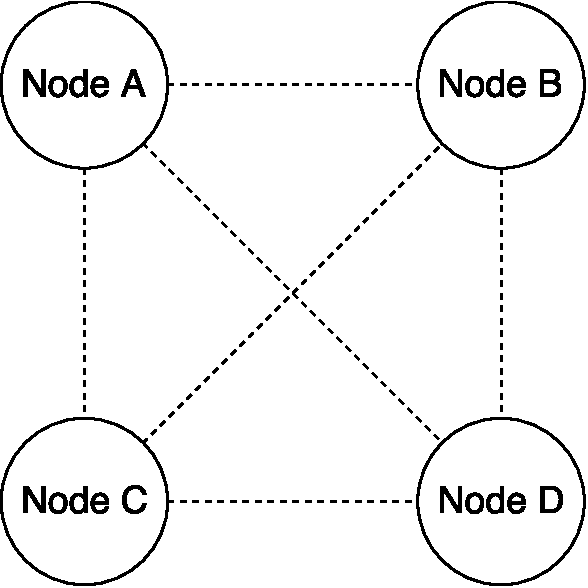
\includegraphics[scale=0.5]{images/computational_environment.pdf}
\caption[Computational environment]{Computational environment, interconnected nodes} \label{fig:computational_environment}
\end{figure}

\subsection{Storage of data} \label{subsec:design_storage}
Information such as how many replicas are currently executing, and on which nodes they are running, must be globally available and accessible from every node in the system.

If information is only stored locally on a node, that information is lost in case that the node fails. In case the information is written to a persistent storage, it may not be lost, but that information will be unavailable until node has been restarted. 

Instead of storing information locally, a remote database can be used. In this case, a single-point-of-failure is introduced, resulting in a system where the reliability is no more than the reliability of the database. If a remote database is used, this must be taken into account in the reliability model.

To achieve a fault tolerant redundant storage of information, a Distributed Hash Table (DHT) can be used. Using DHT efficiently avoids having a single-point-of-failure. 

In Calvin, the framework in which the model was implemented and evaluated, there are two storage alternatives. A DHT implementation called Kademlia, see~\cite{kademlia} for further information, and a proxy storage. Calvin and its storing alternatives is further described in~\cref{subsec:design_calvin}.

%TODO this text needs work
When storing data using DHT, the data is first stored locally and later flushed, i.e. sent to other nodes. When a task is replicated to another node, the replication must only be considered successful if the storage is properly updated and the information shared to other nodes. Otherwise, the replication may only be partially reflected in the storage and use of this data will be useless. 

\subsection{Application model} \label{subsec:design_app_model}
The fault tolerant framework presented in this paper is general and may be used in various contexts. However, it is particularly of value for long running applications and services running in dynamic environments where a predefined level of reliability must be met. Long running applications are particularly vulnerable to failure because they usually require many resources and usually must produce precise results~\cite{relGridSystems}.

In this paper we use a simple application in our experiments, which can be modelled as shown in~\cref{fig:app_model}. The node $A$ shown in the figure could for example be a service for which we require a certain reliability. In contrast to ~\cite{algoOptTimeMaxRel, optTaskAllocationForMaxRel, taskAllocation, taskAllocationSwarm, algoMaxRelEndToEndConstraint, algoMinExTime, schedReplicas}, no assumptions are made about the execution time of the application. While our model is general, it is particularly beneficial for long running applications and services, as they in large-scale distributed environments are required to stay operational even in the case of unpredictable failures~\cite{imprRelAdaptRL}.

A typical example of a long running application is stream data processing, where a continuous stream of data is sent to a service which performs some computations on the data, and sends a result to a receiving process. The execution time is unknown, and in case of a failure, data may be lost. By sending the data to several replicas, redundancy is achieved and reliability thereby increased as the probability of at least one replica produces a result is increased.

\begin{figure}[!hbt]
\centering
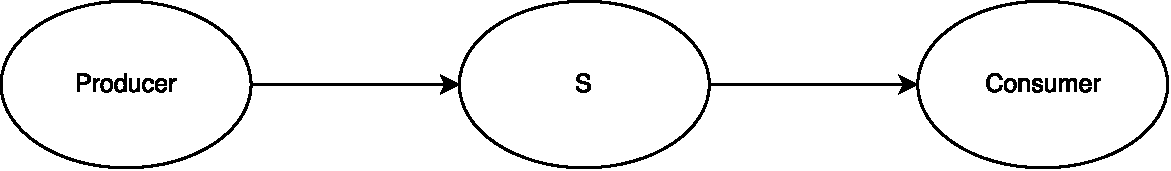
\includegraphics[scale=0.5]{images/app_model.pdf} 
\caption[Application model]{An application model where a producer transmits data to a task $T$, which transforms the data, and sends the result to a consumer. $T$ may be seen as a task or service running in a cluster and requiring a certain level of reliability.}\label{fig:app_model}
\end{figure}

\subsection{Replication scheme} \label{subsec:design_repl_scheme}
As previously mentioned, reliability will be ensured by the use of replication. More specifically, active replication is used, where each replica receives the same input, performs the same computations and produces the same output. \Cref{fig:app_model_replication} shows how the application in \cref{fig:app_model} looks after replicating task $T$ 4 times. It is also possible to have several tasks replicated, this scenario is shown in \cref{fig:extended_app_model}.

In contrast to the case with one \emph{primary} task and several \emph{back-up} replicas, as described in \cref{subsec:background_replication}, we will adapt a fan-in fan-out model, where all replicas both receive the same input, but also all transmit its result to the consumer. %TODO explain fan-in/fan-out in background_replication?

\begin{figure}[!hbt]
\centering
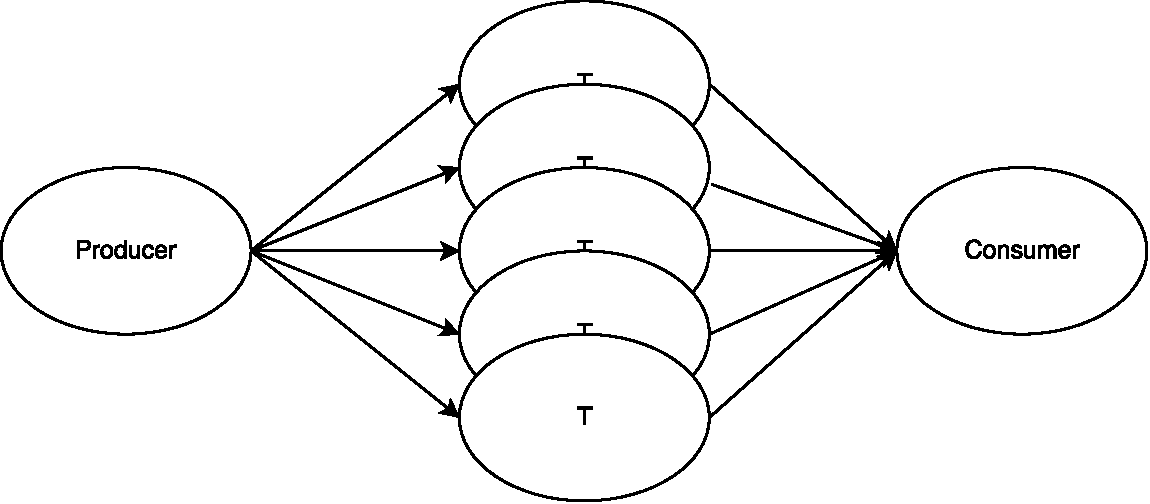
\includegraphics[scale=0.5]{images/app_model_replication.pdf} 
\caption[Application model with replicas]{An application model where a task $T$ has been replicated 4 times.}\label{fig:app_model_replication}
\end{figure}

After replicating, the various replicas may not be synchronized. But, since assuming only deterministic calculations is done by the tasks replicated, given the same input they will all produce the same result, even if not synchronized. However, since the receiver receive a result from each replica, our model allows for easy extension to also include a majority decision at the consumer to determine whether or not the correct result was received. %TODO do we have to have this? I don't think it really affects our model right?

The process of replicating a task in Calvin, the framework in which our model was implemented, is further described in~\cref{subsec:calvin_replication}.

\subsection{Fault model} \label{subsec:design_fault_model}
In this paper, we adapt the \emph{fail-stop} fault model, which is described in~\cref{subsub:background_fail_stop} and commonly used when presenting fault tolerance techniques~\cite{surveyFaultParallel}. Nodes in the system have one of two states: \emph{operational} or \emph{failed}. If a node fails, all running tasks on that node are dead. Furthermore, after a node has died, it will be restarted. However, the tasks that were being executed before it died will not be restarted when the node is restarted. The reason for why a node died is irrelevant.

Like~\cite{selfAdaptRel}, only system related failures are considered, assuming failures depends on the nodes, not the jobs running on them and the computations they perform. Furthermore, unlike the reliability models presented in~\cite{taskSchedulingReplication, taskAllocationSwarm, relAnalysisFRA}, the network is assumed fully reliable, and thus link failures are not accounted for.

\subsubsection{Failure distribution} \label{design:failure_distribution}
A commonly used assumption, also adapted in this paper, is that failures are statistically independent. Furthermore, failures are assumed to follow a Poisson process, as this seems to be widely accepted in the research community~\cite{experimentalFailureAssessment}. 

While most models using the Poisson process to model reliability assume constant failure rates, we assume they are constant only for a given period of time. By monitoring the system resources and registering failure times, the \emph{MTBF} of a node can by dynamically adapted. This is accomplished by using the time of the three latest failures to determine the \emph{MTBF} as of~\cref{def:MTBF}. This is further described in~\cref{sec:design_self_adapting_mtbf}. 

Since we assume the \emph{MTBF} for a node is constant during a period of time, failures can be modeled using a Poisson process. Using a resource's \emph{MTBF}, the reliability for that resource can using~\cref{eq:Poisson} be expressed as
 
\begin{equation} \label{eq:resource_reliability}
R(t) = e^{-t/MTBF}
\end{equation}

\Cref{eq:resource_reliability} expresses the probability that a given resource will work for a time $t$. Correspondingly, the probability that a resource will fail during a time interval of length $t$ is

\begin{equation} \label{eq:resource_failure_prob}
F(t) = 1- e^{-t/MTBF}
\end{equation}

In our case \emph{t} represents the time it take to detect a node failure and create a new replica, and is further discussed in~\cref{sec:design_time_t}.

In order to use~\cref{eq:Poisson_no_failures}, the \emph{MTBF} of a node must be available, and to calculate a node's \emph{MTBF} at least two failures must have occurred since not all nodes are alive at time zero which is assumed by~\cref{def:mttf}. However, the system still need to be able to calculate the reliability for a node, even if the node has not yet failed. Therefore, a default value for the \emph{MTBF} will be used in the experiments when no failure data is available for a node, or if it has not yet failed twice. In a real situation, the default value could be based on past failure data for resources of similar type. The default value used in the experiments is further described in~\cref{sec:eval_values}.

As time goes and nodes fail, the time of failure for nodes are stored, the system will get more precise values for the \emph{MTBF} for the nodes in the system. By using the latest three failure times, one can adapt the \emph{MTBF} as nodes start failing more or less often. 


\section{Monitoring} \label{sec:design_monitoring}
Monitoring the system is crucial for achieving an entirely dynamic system, both in which the required reliability is met over time, but also not to use more resources than necessary. 

\subsection{Heartbeats} \label{subsec:heartbeats}
The ability to detect node failures is crucial for knowing when a new replica is needed in order to keep the required reliability. Furthermore, since the reliability model presented in~\cref{sec:design_reliability_model} is based on a \emph{mean-time-between-failures} for the nodes in the system, it is based on the assumption that node failures are detectable. 

To achieve this, a heartbeat system is used, where nodes periodically send UDP messages, called heartbeats, every $t_h$ seconds. The heartbeats contain a node identifier and are sent to all the other nodes in the system. Nodes are considered operational as long as heartbeats are received from them, and if no heartbeat is received from a node for $t_{timeout}$ seconds, the node is assumed dead.

In the experiments conducted, see \cref{ch:evaluation}, $t_h$ was set to 0.2 seconds, and $t_{timeout}$ to 0.5 seconds. These values should be modified in a real setting. For the experiments, a high-bandwidth low-latency cluster was used, why we could use a high heartbeat frequency and a low timeout time.

As further described in~\cref{sec:node_failure_detection_time}, these values affect the reliability model, and thereby the number of replicas needed. A higher frequency and lower timeout means a shorter time in which the system is in a vulnerable state, and therefore a lower number of replicas may be needed to reach the required reliability. On the other hand, higher frequency means increased network traffic in the system as more heartbeats are being sent, although the size of a heartbeat message is low, only 126 Byte.

\subsection{Monitoring system reliability} \label{subsec:monitoring_system_rel}
In order to ensure the optimal number of replicas is used over time, as the properties of the system varies, the system and its running applications or services must be periodically monitored. 

In our model, the reliability of the running applications are monitored periodically, and if the reliability is not met, appropriate actions are taken, which is further described in~\cref{sec:design_sched_alg}.

On the other hand, if the required reliability is met, more replicas than necessary may be used to reach that reliability level. One must therefore minimize the number of replicas by moving the replicas to more reliable nodes, and deleting replicas on less reliable nodes as long as the required reliability is still met. The algorithm for optimizing is further described in~\cref{subsec:design_optimization}.

In the experiments, all applications were monitored and the greedy scheduling algorithm followed by the optimization algorithm, both presented in~\cref{sec:design_sched_alg}, were run every five seconds.

\section{Reliability model} \label{sec:design_reliability_model}
In this section the reliability model used in our experiments is presented. Note that the scheduling algorithm presented in~\cref{sec:design_sched_alg} is not dependent on the reliability model used.

\subsection{Definitions} \label{subsec:design_definitions}
In this paper, we use the following definitions of reliability:
\begin{definition} \label{def:single_task_reliability}
The reliability of a process is the probability that the resource on which the process is running is functioning during the time of execution.
\end{definition}

For long running applications or services, where a replication scheme is used and new replicas dynamically being created as old ones fail, the reliability can be defined as \cite{effTaskReplMobGrid}

\begin{definition} \label{def:task_replica_reliability}
The reliability of a process, with $n$ task replicas, is the probability that at least one replica is always operational. This can be expressed as the probability that not all replicas fail during the time from that a task replica dies, until a new replica is operational.
\end{definition}

\subsection{Expressing reliability}\label{subsec:design_reliability}
Using replication and the reliability definition defined in~\cref{def:task_replica_reliability}, the reliability of a task $T$ with $n$ replicas, is the probability that at least one replica is successful during a time $t$, where $t$ is the time from that a replica fails, until a new replica is operational. This corresponds to at least one replica surviving time $t$, i.e. not all replicas fail, and can be expressed as 

\begin{equation} \label{eq:task_reliability}
R_{T}(t) = 1 - \prod\limits_{k=1}^n f_{k}(t)
\end{equation}

where $f_{k}(t)$ is the probability that replica $k$ fails during time $t$. 

Since assuming tasks themselves do not fail unless the resources they use fail, the reliability of a task is dependent on the reliability of the resources it uses, not the number of replicas. Considering only node failures, the reliability of a task $T$ with $n$ replicas placed on $m$ different nodes, can using~\cref{eq:resource_failure_prob} be expressed as

\begin{equation} \label{eq:task_reliability_2}
R_{T}(t) = 1 - \prod\limits_{k=1}^m F_{k}(t) = 1 - \prod\limits_{k=1}^m (1- e^{-t/MTBF_k})
\end{equation}

Where $MTBF_k$ is the \emph{mean-time-between-failure} for node $k$. Using this model, reliability is only increased through replication if the replicas are scheduled on separate nodes. Furthermore, \cref{eq:task_reliability_2} is based on the assumption that failures of nodes are statistically independent, which is a commonly used assumption as described in~\cref{subsec:background_failure_distribution}.

Given a time $t$, a required reliability level $R_{req}$, and assuming the replicas are running on $m$ separate nodes, we get

\begin{equation} \label{eq:required_rel}
R_T(t) = 1 - \prod\limits_{k=1}^m F_{k}(t) \geq R_{req}
\end{equation}

which must be fulfilled by the system. Assuming that failure rates differ among resources, fulfilling \cref{eq:required_rel} is a scheduling problem, since the number of replicas needed is dependent on which resources the replicas are running on.

The scheduling problem to fulfill a reliability $R_{req}$ refers to selecting $m$ nodes on which to place $m$ replicas such as the reliability level of the task, expressed in \cref{eq:task_reliability_2}, exceeds $R_{req}$.

\subsection{Expressing time t} \label{sec:design_time_t}
The time $t$ used in \cref{eq:task_reliability_2} is the time it takes from that a failure happened, until a new replica is operational, and consists of the time it takes to detect the failure, and the time it takes to create a new replica. The time $t$ can therefore be expressed as 

\begin{equation} \label{eq:rep_time}
	t = t_d + t_R
\end{equation}

where $t_d$ is the time to detect that a node has failed, and $t_R$ is the time it takes to create a new replica. A new replica is created by sending a replication request to a node currently holding a replica, including a third node on which the new replica is to be created. This process is further described in~\cref{sec:replication_time}.

\subsubsection{Node failure detection time, $t_d$} \label{sec:node_failure_detection_time}
As described in~\cref{subsec:heartbeats}, heartbeats are periodically sent to all nodes in the system every $t_h$ seconds, and if no heartbeat is received from a node for $t_{timeout}$ seconds, it is assumed dead. Note that $t_h$ must be lower than $t_{timeout}$.

The timeout time, $t_{timeout}$ is only an upper bound for how long it takes to detect a node failure. A node may fail just before sending a heartbeat, or directly after, which will affect the actual time the node has been dead before it is detected. This corresponds to the best and worst case scenario. 

If a node A dies precisely before sending heartbeat $H_k$ to node B, the last received heartbeat from A was $H_{k - 1}$. $t_{timeout}$ seconds after $H_{k - 1}$ was received, node B will assume A has failed. Node A will then have been dead for $t_{timeout} - t_h$ seconds.

In the latter case, node A dies directly after sending a heartbeat $H_k$, and $t_{timeout}$ seconds later node B will assume node A has failed. Node A has in this case been dead for $t_{timeout}$ seconds when node B assumes it has failed.

Assuming that the probability of a node dying just before and directly after sending a heartbeat is the same, we get a theoretical average detection time of $t_{timeout} - \frac{t_h}{2}$ seconds. 

An example of the best and worst case scenario is shown in~\cref{fig:heartbeats_best_case} and~\cref{fig:heartbeats_worst_case}.

In~\cref{eq:rep_time} we will use

\begin{equation} \label{eq:node_failure_detection_time}
t_d = t_{timeout}
\end{equation}

which is the worst case scenario. This result in the calculated reliability always being equal to or lower than the actual reliability, since the time to detect the failure always is $t_{timeout}$ or lower.

\subsubsection{Replication request time, $t_R$} \label{sec:replication_time}
The time $t_R$ in~\cref{eq:rep_time} is the time from that a replication request is sent, until a new replica is operational and a response is received. It consists of the time it takes to send a replication request to a node, for that node to replicate its replica to another node and send a response.

To know which node to send the replication request to, one must first find out on which nodes current replicas are running. Thereafter, since the reliability is dependent on which nodes the replicas are running on, not solely on the number of replicas, one must also find a node which has no replica already and include this in the request. The time $t_R$ can be expressed as in~\cref{eq:replication_request_time} where $t_{query\ storage}$ is the time it takes to find which nodes currently holding a replica and which nodes does not, $t_{replicate\ msg}$ is the time to send a replication message to another node, $t_{r}$ is the time to replicate the task to another node, and $t_{response}$ is the time to send a response to the requesting node. The process of sending a replication request is shown in~\cref{fig:replication_request}. The part of querying the storage is excluded from this figure.

\begin{equation} \label{eq:replication_request_time}
t_R = t_{query\ storage} + t_{replicate\ msg} + t_{r} + t_{response}
\end{equation} 


\begin{figure}[!hbt]
\centering
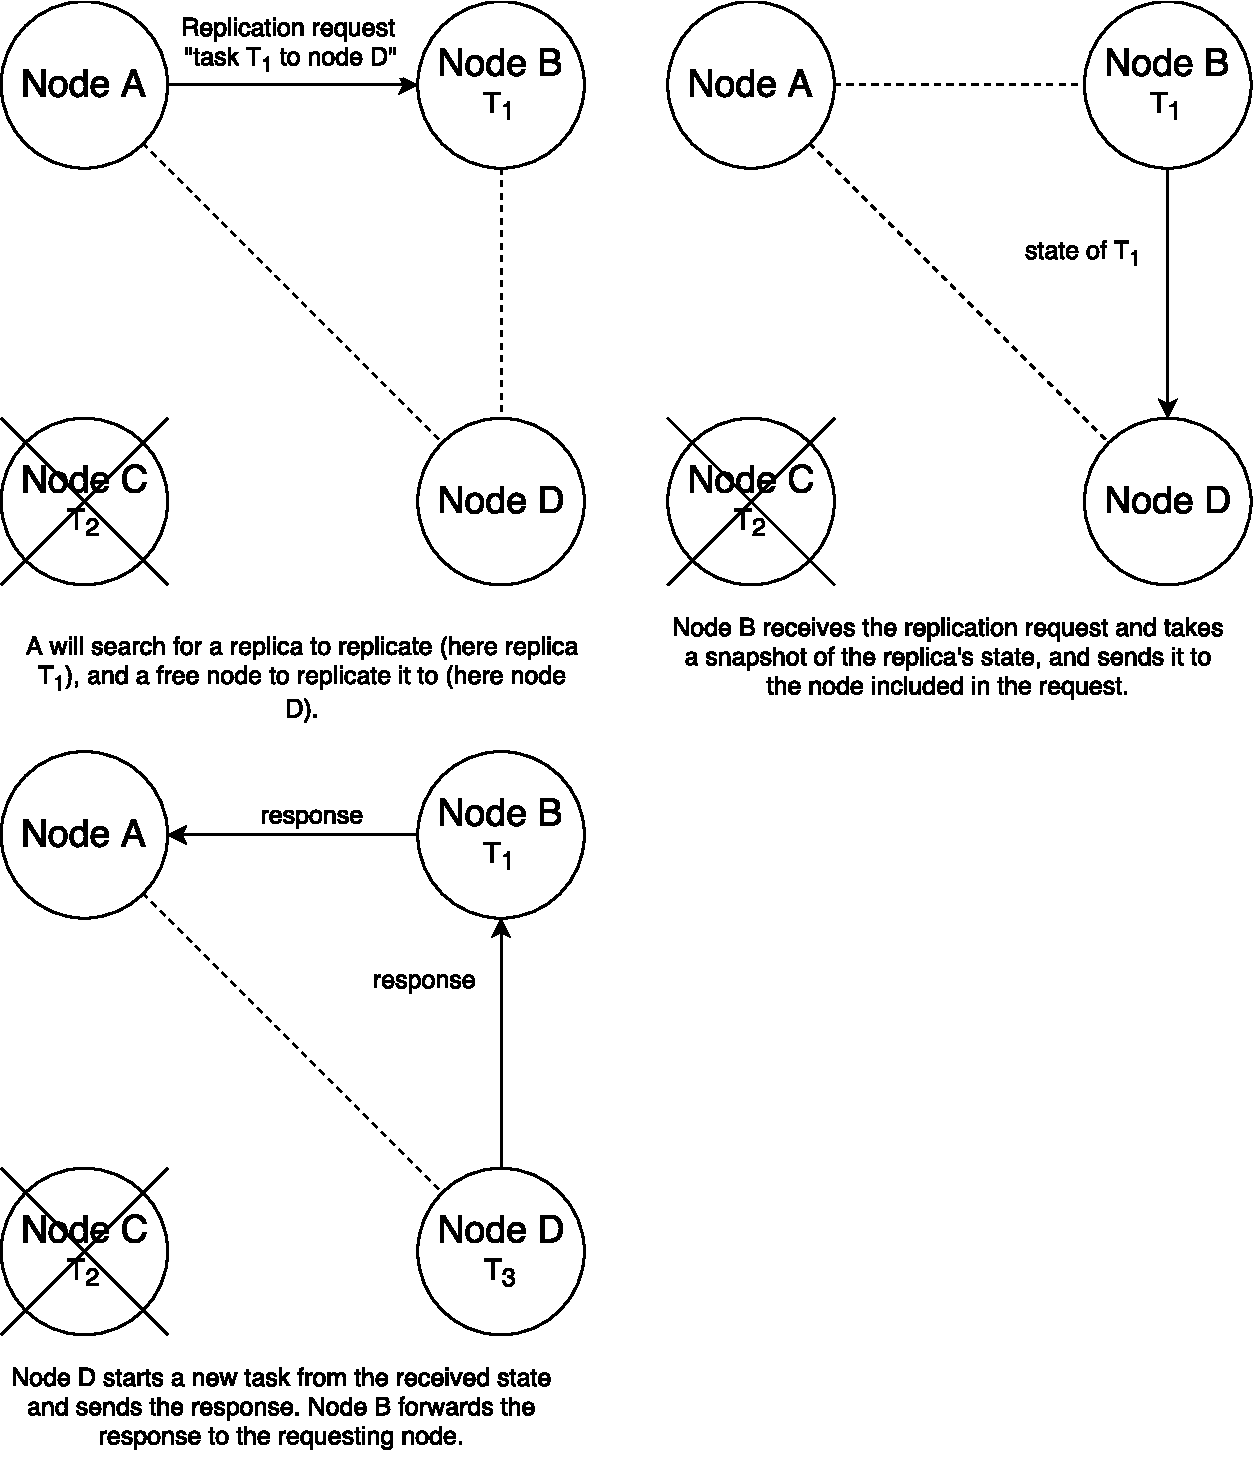
\includegraphics[scale=0.5]{images/replication_request.pdf}
\caption[Replication request]{The process of node A asking node B to replicate its replica $T_{1}$ to node C, and receiving a response.}\label{fig:replication_request}
\end{figure}

As mentioned, the time $t_r$ is the time it takes to replicate a task. Depending on the state of the task to replicate, it is likely to be a significant part of the total time $t_R$. The time to replicate a task consists of the time to get the state of the task, serialize it, transmit it to the other node, de-serialize it, and create a new identical replica using that state, and send the response. 

\begin{equation} \label{eq:replication_time}
t_{r} = t_{get\ state} + t_{serialize\ state} + t_{transmit\ state} + t_{de-serialize\ state} + t_{create\ new} + t_{send\ reply}
\end{equation} 

In our model, the time $t_{R}$ is measured and stored every time a replication takes place. Since $t_{r}$ depends on the size of the state, the time to replicate different tasks are likely to vary. Therefore, the time $t_{R}$ is stored per task type. Consequently, different types of tasks may require different number of replicas to reach the same reliability, as the reliability is dependent on the time $t_R$. \Cref{fig:replicas_depending_on_t} shows how the number of replicas needed to reach a reliability above 0.99, using nodes with a \emph{MTBF} of 10 seconds, vary depending on the time \emph{t}.

\begin{figure}[!hbt]
\centering
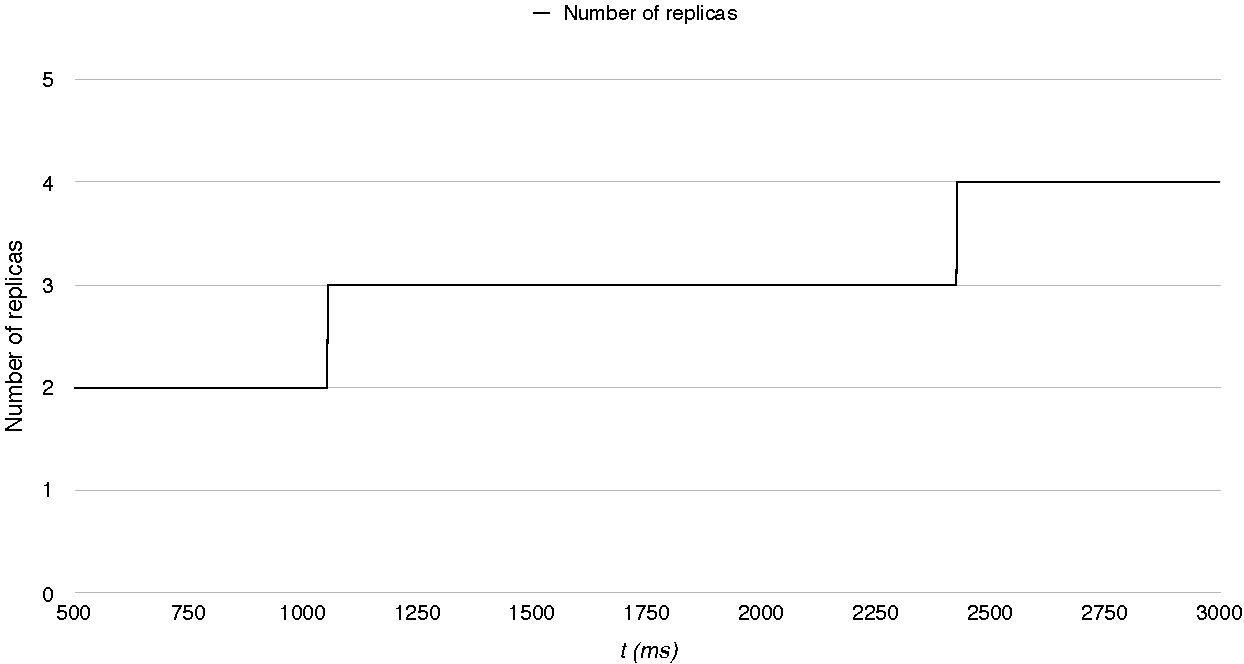
\includegraphics[scale=0.5]{images/replicas_depending_on_t.pdf}
\caption[Number of replicas needed]{The number of replicas needed to reach a reliabilty above 0.99, using nodes with a \emph{MTBF} of 10 seconds, depending on the time $t_{r}$.}\label{fig:replicas_depending_on_t}
\end{figure}

Other factors affect the time $t_R$. The node to which the replication request is sent may die before the replication is finished. The sender of the request assumes the receiving node has failed if no response is received within a timeout time. In this case, a new node is selected and asked to replicate its replica. When this happens, the time $t_R$, will be relatively high, as time was wasted sending the request to the first node.

This situation can theoretically continue until there is no more nodes holding a replica. One could argue that this should be taken into account in the reliability model, as the time $t_R$ affects the reliability. Also the node being selected to run~\cref{alg:scheduling}, described in~\cref{sec:design_handling_failure}, may die, in case a new node is selected. These situations are further described in~\cref{sec:design_handling_failure}. The probability of these situations happening depend on how often nodes fail, and how long time the replication takes. If nodes fail very frequently, there is a higher risk of a node failing before finishes the replication.

Instead of including the probability of these situations in the reliability model, a log-logistic distribution is first fitted to the previously registered times $t_R$. From the fitted distribution, the 95th percentile value is used as the value for $t_R$ in~\cref{eq:rep_time}. This means in 95 percent of the cases, the time $t_R$ will actually be lower than the value used in~\cref{eq:rep_time}. The reason for choosing log-logistic distribution is mentioned in~\cref{sec:eval_time_t}.

Finally, since assuming that all nodes are within the same cluster and that the latency between all nodes are low, we assume the time $t_R$ is independent on between which nodes the replication takes place. 

\section{Scheduling algorithm} \label{sec:design_sched_alg}
To fulfill~\cref{eq:required_rel} using the minimum number of replicas, one could simply place a new replica on the most reliable node available, until the required level is reached. A greedy scheduling algorithm doing this, similar to one presented in~\cite{effTaskReplMobGrid}, and which fulfills~\cref{eq:required_rel} is shown below:

\begin{algorithm}[H]
	\caption{Greedy scheduling algorithm to fulfill a given reliability} \label{alg:scheduling}
	\begin{algorithmic}[1]
	\Require{$R_{req}$ is the reliability to fulfill.}
	\Statex
	\Procedure{Greedy scheduling algorithm}{}
	\State $current\ nodes\gets$ current nodes
	\State $operational\ nodes\gets $ operational nodes
	\State $available\ nodes\gets operational\ nodes \setminus \ current\ nodes$
	\State
	\Call{sort}{$available\ nodes$, $descending$}
	\While {\Call{reliability}{$current\ nodes$} $\leq R_{req}$}
		\State $node\gets available\ nodes.pop$\Comment{take the most reliable node}
		\State{$replica\gets new\ replica$}
		\State
		\Call{place replica on node}{$replica$, $node$}
		\State $current\ nodes.add(node)$
	\EndWhile
	\EndProcedure
	\end{algorithmic}
\end{algorithm} 

\begin{function} 
	\caption{Sorts the given nodes in order of preference} \label{func:sort}
	Returns the given nodes in sorted order, with the most or least (depending on $order$) preferred nodes first. We only consider the nodes' reliability when sorting, but it can easily be changed to consider other parameters as well.
	\begin{algorithmic}[1]
	\Ensure{$nodes$ is the list to sort, and $order$ is the order to sort in (ascending or descending).}
	\Statex
	\Function{sort}{$nodes$, $order$}
		\State
	    \Call{sort after reliability}{$nodes$, $order$}
	    \State \Return $nodes$
	\EndFunction
	\end{algorithmic}
\end{function}

\begin{function} 
	\caption{Calculates the reliability of the given nodes} \label{func:calc_reliability}
	Calculate the reliability of the nodes currently holding a replica. This function could be change to use a different reliability model.
	\begin{algorithmic}[1]
	\Ensure{$current\ nodes$ is a list of nodes currently holding a replica.}
	\Statex
	\Function{reliability}{$current\ nodes$}
		\State $n\gets current\ nodes.length$
		\State return $ 1 - \prod\limits_{k=1}^n (1 - R_{current\ nodes[k]}(t))$
	\EndFunction
	\end{algorithmic}
\end{function}

In our model, a new replica is placed on the most reliable node until the required reliability level is reached. However, we do not account for whether or not the selected node has enough available resources for the new replica, hence we do not consider system load. The scheduling algorithm is however independent of both the selection of nodes, \cref{func:sort}, and the calculation of the current reliability, \cref{func:calc_reliability}, why these two are two separate function calls. 

In our model, the reliability function uses~\cref{eq:task_reliability_2} for determining the reliability, and the sort function simply sorts available nodes after reliability, but they could both easily be replaced by more sophisticated models, e.g. which also consider nodes' loads when sorting them.

The algorithm is run when deploying an application, when a failure is detected as further described in~\cref{sec:design_handling_failure}, and also periodically in combination with an optimization algorithm, described next in \cref{subsec:design_optimization}.

\subsection{Optimization} \label{subsec:design_optimization}
\Cref{alg:scheduling} creates the minimal number of new replicas needed to reach the required reliability. However, it does not ensure that the minimum number of replicas is used over time. As more reliable nodes become available, fewer replicas could be used while still meeting the required reliability. Therefore, \cref{alg:optimization} is periodically run, as part of the application monitoring as described in~\cref{subsec:monitoring_system_rel}. By first running the greedy scheduling algorithm, and then the optimization algorithm, we ensure both that the required reliability is met, and that it is met while using the minimum number of replicas possible.
 

\begin{algorithm} 
	\caption{Optimization algorithm} \label{alg:optimization}
	\begin{algorithmic}[1]
	\Procedure{Move to most reliable nodes}{}
	\State $current\ nodes\gets $ current nodes
	\State $operational\ nodes\gets $ operational nodes
	\State $available\ nodes\gets operational\ nodes \setminus \ current\ nodes$
	\State
	\State
	\Call{sort}{$available\ nodes$, $descending$}
	\State $most\_reliable\gets available\ nodes.pop$
	\State
	\Call{sort}{$current\ nodes$, $ascending$}
	\State $least\_reliable\gets current\ nodes.pop$
	\State
	\While{$R_{most\_reliable}(t) > R_{least\_reliable}(t)$}
			\State $replica\gets $\Call{replica at}{$least\_reliable$}
			\State
			\Call{replicate to}{$replica$, $most\_reliable$}
			\State
			\Call{delete replica from node}{$replica$, $least\_reliable$}
			\State
			\State $current\ nodes.add(most\_reliable)$
			\State $available\ nodes.add(least\_reliable)$
			\State $least\_reliable\gets current\ nodes.pop$
			\State $most\_reliable\gets available\ nodes.pop$
	\EndWhile
	\EndProcedure
	\State
	
	\Procedure{Delete unnecessary replicas}{}
	\State $least\_reliable\gets current\ nodes.pop$
	\While {\Call{reliability}{$current\ nodes$}\ $\geq R_{req}$}
		\State $replica\gets $\Call{replica at}{$least\_reliable$}
		\State
		\Call{delete replica from node}{$replica$, $least\_reliable$}
		\State $least\_reliable\gets current\ nodes.pop$
	\EndWhile
	\EndProcedure
	\end{algorithmic}
\end{algorithm}

The first part of~\cref{alg:optimization} makes sure the most reliable nodes are used, by moving the replicas on the least reliable nodes to the most reliable nodes available, as long as more reliable nodes are available. To avoid putting the system in a vulnerable state, moving a replica involves first creating a new replica, and later deleting the old one. If deleting before creating the new replica, one risk not having enough replicas until the new replica is operational. Replicating first avoids this problem.

The second part make sure no unnecessary replica is used, by deleting the replica on the least reliable node as long as the required reliability is still met.

\Cref{alg:optimization} makes sure no unnecessary replicas are used. However, moving replicas to more reliable nodes may be unnecessary overhead if it does not affect the overall number of replicas needed. For example, moving from a node with a reliability of 0.999 to a node with reliability 0.9991 will perhaps not significantly increase the overall reliability, and if it does not result in another replica can be deleted, it may be unnecessary. \Cref{alg:optimization} does not account for this.

\section{Handling node failure} \label{sec:design_handling_failure}
In the case of a node failure, one must first determine whether or not any replicas were running on the failed node, and if so, determine whether or not new replicas are needed to still fulfill the required reliability level. This is accomplished by running~\cref{alg:scheduling}. However, when a node fails, all other nodes in the system will detect its failure, since no node will receive heartbeats from it. If all other nodes start running~\cref{alg:scheduling}, one could end up in a situation where every remaining node creates a new replica. While this will increase the reliability, it may result in an unnecessarily high number of new replicas being created, thus the optimal number of replicas will no longer be used.

To cope with this, a selection process must take place in which a single node is selected, which will be responsible for deciding what actions to take. Since assuming a dynamic system where nodes fail and new nodes are introduced, this selection must be done every time a node dies. Furthermore, the selected node may also die before it manages to create any new replica. Therefore, all nodes will send a \emph{lost node} request to the selected node. When finished, the selected node sends a reply back to all nodes it received a \emph{lost node} message from. If the sending nodes do not receive a reply within a timeout, they assume the selected node died, and a new selection process will begin.

The algorithm is shown below:

\begin{algorithm}[!h]
	\caption{Handling a failed node} \label{alg:node_failure}
	\begin{algorithmic}[1]
	\State $operational\ nodes\gets $ operational nodes
	\State $lost\ node\ id\gets $ lost node id
	\State
	\Call{sort after ID}{$operational\ nodes$}
	\Do
		\State $node\gets operational\ nodes.pop$
		\State
		\Call{lost node request}{$node$, $lost\ node\ id$}
		\State {wait for reply}
		\State $reply\gets reply\ from\ node$
	\doWhile {$reply\ is\ not\ successful\ OR\ request\ timeout$}
	\end{algorithmic}
\end{algorithm}

A small example is presented in~\cref{fig:handling_node_failure}. In the situation shown in the figure, there are 4 connected nodes, A, B, C and D, and the node C has just failed. When the other nodes (A, B and D) detect the failure they will select the node with the highest ID, in this case node A, and inform it that node C has failed. Node A will then determine which actions to take.

\begin{figure}[!hbt]
\centering
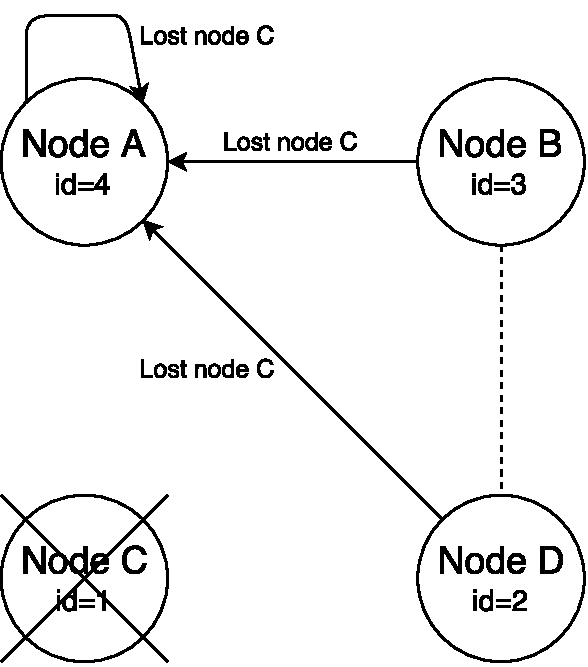
\includegraphics[scale=0.5]{images/handling_node_failure.pdf}
\caption[Handling a node failure]{4 interconnected nodes after nodes A, B and D have detected the failure of node C.}\label{fig:handling_node_failure}
\end{figure}

\subsection{Selecting node}
As described, the node responsible for handling the detected failure is the node with highest ID among the nodes still being operational.

If the selected node determines a new replica is needed, it will send a replication request to a node currently holding a replica. If the selected node is one of the nodes holding a replica, there is no need for a replication request, since the node could simply replicate its own replica. One could therefore get rid of a replication request if one selected a node currently holding a replica in the selection process. However, to find out which nodes currently hold a replica, one must query the storage used, as described in~\cref{sec:replication_time}. Whether or not a centralized database is used, or DHT as used in Calvin where our model was implemented, this would result in every node detecting the failure querying the storage, and this approach is not scalable. Therefore, the selected node is any of the nodes still operational, and solely the selected node will query the storage for the information needed to handle the failure.

\section{Self-adapting} \label{sec:design_self_adapting}
Adaption refers to changing the behavior as the state of the system changes. For a distributed system, resources most be continuously monitored in order to adapt to changing behavior~\cite{imprRelAdaptRL}.

To ensure a certain level of reliability, the framework must ensure that the current state of the system is taken into account when determining the number of replicas needed. Furthermore, the system and the running jobs must be continuously monitored. If the reliability of a running application task decreases below the required level, more replicas must be created. On the other hand, if the reliability increases, the number of replicas should be decreased in order not to waste resources, as long as doing so does not result in a reliability lower than the required one.

When monitoring the system, all parameters used in the reliability model must be monitored. In our case, we consider only the nodes' mean-time-between-failures, the time to detect node failures and the time it takes to create a new replica. Therefore, all nodes' failure times, and the time to create new replicas are registered. The time to detect failure is as mentioned in~\cref{sec:node_failure_detection_time} static.

\subsection{Adapting time $t$}
Since using all registered times $t_R$ to fit the log-logistic distribution, and selecting the 95th percentile value as described in~\cref{sec:replication_time}, the value of $t_R$ used in~\cref{eq:rep_time} will depend on all previous registered values. Therefore, if the replication time starts increasing, e.g. during higher system load, the value used in the reliability model will also increase, thereby adapting to changing behavior. 

\subsection{Adapting nodes' \emph{MTBF}} \label{sec:design_self_adapting_mtbf}
As described in~\cref{design:failure_distribution}, only the three latest failure times for a node are used to determine its \emph{MTBF}. This allows for adapting a node's \emph{MTBF} in case it starts failing more or less often. 

However, if a node starts dying more often, the model needs three new failure times before the \emph{MTBF} has been update to correctly reflect its new behavior. This is a clear limitation to our model. Instead, the past failure times could be used together with some machine-learning algorithm or statistical regression, to predict when a node is about to fail more or less often, and adapt its \emph{MTBF} before it actually happens.

\section{Implementation} \label{sec:design_implementation}
For implementing our model, we use an actor based application environment called \emph{Calvin}. Below follows a brief description of the main parts of the Calvin framework, for further info we refer to~\cite{calvin}.

\subsection{Calvin} \label{subsec:design_calvin}
Calvin is an actor-based application environment for light-weight IoT applications, and is written in Python. It was developed by \emph{Ericsson} and made open source in the summer of 2015. While Calvin is an application environment for IoT applications, is suites well for implementation of our model.

The main features of Calvin is the use of runtimes (containers) in which actors (application tasks) run. Since the runtimes separate the hardware from the software, it is possible to use Calvin on different platforms. In developing phase of new applications the developer does not need to consider on which operating systems the application should run.

\subsubsection{Storage} \label{sec:calvin_storage}
In Calvin there are two ways of storing data, either by the Kademlia implementation of a DHT or by the use of a proxy storage.

Using Kademlia, data is stored both locally and remotely, by distributing the data to other nodes in the system. The data is therefore available despite one of the storing nodes fails. One of the configurable parameters used in Kademlia is $k$, representing the maximum size of a bucket-list. The value of $k$ should be chosen such that the probability of $k$ nodes failing within an hour is very low \cite{kademlia}. DHT will not be further explained in this thesis, instead we refer to~\cite{kademlia} for further information about DHT and Kademlia especially. 

When using the proxy storage, one runtime acts as a storage node, and all data is sent to that runtime. All requests for data is also sent to the runtime acting as proxy storage. However, the proxy storage introduces a single point of failure, since all data is lost if that runtime fails. %TODO mention some pros, eaiser when testing?

\subsubsection{Actor model} \label{sec:calvin_actor}
An application in Calvin consist of a set of connected \emph{actors}. An actor usually represents part of a device, service or computation. Actors communicate by sending data, called tokens, on their out-ports to other actors in-ports. 

Multiple actors may send data to another actor's in-port, and an actor's out-port may have several receivers. For each receiver of outgoing messages, or sender of incoming messages, there is a separate queue of tokens to process.

The runtime, see~\cref{sec:calvin_runtime}, in which an actor is executing is responsible for the communication between runtimes and between actors.

The state of an actor is needed when replicating an actor. In Calvin, the state of an actor consists mainly of actor type, in-port and out-port connections, and for each port a queue with data to process or to send, and read and write positions for the incoming and outgoing queues. The queues is the major part of the message size.

The actor model corresponds well to the kind of applications and tasks described in~\cref{subsec:design_app_model}, as they perform deterministic calculations.

\subsubsection{Runtimes} \label{sec:calvin_runtime}
The Calvin framework use a concept of \emph{runtimes}. A mesh of connected runtimes makes up the distributed execution environment on which one can deploy application. A runtime is a self-managed container for application actors and provides data transport between actors both within the same runtime and between different runtimes.

Each runtime has a \emph{storage}. If DHT is used, all the information in the storage is first stored locally and later flushed, i.e. distributed in a multicast approach. If a proxy storage is used, the information is also stored locally at first, but later flushed to the proxy storage only.

%TODO
In our model a runtime corresponds to a node.

\subsubsection{Replication} \label{subsec:calvin_replication}
The process of replicating an actor in Calvin starts with getting the state of the actor to replicate, serializing it and sending it to the runtime in which the new replica is to be created. The receiving runtime then de-serializes the state and uses it to create the replica and setup its port connections.

Part of creating the new replica is decoding the in- and out-ports' queues, which are part of the state. This processing is CPU bound and affects the total replication time, as shown in the experiment in~\cref{sec:eval_repl_time}.

\subsection{Our contributions to Calvin} \label{subsec:design_contributions} % ish?
Here follows a description of the most important parts of our changes and new features in Calvin.

\subsubsection{Fan-in connectivity}
We extended the Calvin framework to allow a fan-out/fan-in connectivity model where actors can have multiple producers (fan-in) and multiple consumers (fan-out). Previously, only multiple receivers were allowed, but with our changes an actor's in-port could have multiple senders.

\subsubsection{Actor replication}
Previously, the framework allowed for dynamically migrating an actor from one runtime to another. We extended this functionality by allowing dynamic replication of actors. 

\subsubsection{Node Resource Reporter}
To share various kinds of resources between runtimes, e.g. CPU usage as used in~\cref{sec:eval_replaceable_model}, we created a resource reporter actor. When a runtime is created, it automatically creates a resource reporting actor. The actor periodically reports the node's CPU usage to all connected runtimes. 

\subsubsection{Heartbeat Actor}
The heartbeat system described in~\cref{subsec:heartbeats}, was implemented using actors. Each runtime creates a heartbeat actor when its started. The heartbeat actor listens for heartbeats as well as periodically sends heartbeats to other runtimes.

Unlike the resource manager, messages are sent using UDP instead of TCP. With TCP, an initial handshake it used to setup the communication channel. For a heartbeat system, this is unnecessary overhead. 

For every heartbeat received, a timeout of $t_{timeout}$ seconds is set, and when it times out, the runtime to which the heartbeat was sent is assumed dead. On the other hand, when a heartbeat is received, all timeouts related to that runtime is canceled. When a timeout happens, \cref{alg:node_failure} is deployed and new replicas are created if needed to reach the required reliability, see~\cref{sec:design_handling_failure}.

\subsubsection{Application monitor}
Each runtime also periodically monitors the applications deployed to it, to ensure the required reliability is achieved by running \cref{alg:scheduling} and creating new replicas if needed. Also the optimization algorithm, is run as part of this monitoring.
%TODO Mention what happens if the runtime which deployed the application dies?

\chapter{Evaluation} \label{ch:evaluation}
In order to validate our model, we conducted a set of experiments. The goal of the experiments was to show the three main properties of our model. Firstly, that it dynamically ensures the required level of reliability is met, despite the event of node failures, by dynamically creating new replicas when old ones are lost. Secondly, that it uses the optimal number of replicas by choosing the most reliable nodes, and also removing unnecessary ones. Thirdly, that it adapts to changing properties of the system. 

We also measured the time $t_R$ to find the best fitting distribution for these values, and also the replication time $t_r$ for varying state sizes. Finally, we measured the actual time for detecting failure to demonstrate that the values lie between the best and worst case described in~\cref{subsec:heartbeats}.


\section{Values used in the experiments} \label{sec:eval_values}
As described previously, heartbeats were sent every 200 ms in the experiments, and nodes were considered dead if no heartbeat was received for 500 ms. Furthermore, the optimization algorithm was run every 5 seconds.

As described in~\cref{sec:design_reliability_model}, the reliability model is based on a node's \emph{MTBF} and the time $t_R$. In order to determine the \emph{MTBF} for a node, at least two failure times must have been registered. Before a node has failed twice, a default value is used. The default \emph{MTBF} used in the experiments was 10 seconds.

In addition to the \emph{MTBF}, a default value for $t_R$ must be used before any such times have been registered. The default value used in the experiments was 2 seconds.

The state size of the actor replicated in the experiments was 1901 bytes.

\section{Computational environment} \label{sec:eval_comp_env}
In the experiments, a cluster consisting of 6 inter-connected servers with homogeneous hardware components were used. A laptop was also used when measuring the replication time $t_r$. The specification of the servers and the laptop are described in~\cref{sec:server_spec} and \cref{sec:laptop_spec}. The various servers will be referred to as \emph{Gru}, \emph{Dave}, \emph{Kevin}, \emph{Mark}, \emph{Jerry} and \emph{Tim}.

As mentioned in \cref{ch:design}, the model was implemented in the IoT application environment Calvin. In the experiments, one or two, depending on experiment, Calvin runtimes were started on five of the six servers. These runtimes were used to represent actual nodes, and were periodically killed and restarted to simulate node failure. These five servers are referred to as the unstable servers.

On the sixth server, \emph{Gru}, two runtimes were started which were never killed. One of these stable runtimes was used as a proxy storage, further described in~\cref{sec:eval_storage}, and the reason for having the other stable runtime is described in~\cref{sec:eval_application}. The proxy storage was started in every experiment and the other stable runtime was started in every experiment expect the one where we measured the actual time for detecting failures.

In the experiments, the runtimes are referred to as nodes, and when referring to creating nodes with a specific \emph{MTBF}, we refer to the runtimes created on the 5 unstable servers.

\subsection{Simulating node failure} \label{sec:simulating_node_failure}
As mentioned, the servers used in the experiments had homogeneous hardware components, but varying failure rates were simulated by killing and restarting the runtimes with varying rates.

The process of killing and restarting is shown in~\cref{alg:simulating_node_failures}. If a node was to have a \emph{MTBF} of 15 seconds, the time between failures followed a normal distribution with mean 15 and standard deviation of 1. 

Since the experiments only ran for less than 30 minutes, the actual \emph{MTBF} for a given node may during the duration of a experiment be either lower or higher than the given \emph{MTBF}. The reason for using values from a normal distribution with a mean equal to the given \emph{MTBF}, instead of a fixed time, was to simulate a more realistic situation. If all runtimes would have been started at the same time, with the same fixed time to sleep before killing them, they would all have been killed at the same time. Furthermore, if we would have waited some time before starting each runtime, two runtimes would perhaps never have died at the same time. By picking values from a normal distribution, two or more runtimes may fail at the same time during the time of the experiments.

\begin{algorithm} 
	\caption{Simulating node failures} \label{alg:simulating_node_failures}
	\begin{algorithmic}[1]
	\While {$true$}
		\State
		\Call{start runtime}{}
		\State $t_{s}\gets \mathcal{N} (MTBF,1)$
		\State
		\Call{sleep $t_{s}$}{}
		\State
		\Call{kill runtime}{}
	\EndWhile
	\end{algorithmic}
\end{algorithm}

\subsection{Node specification}
\subsubsection{Server specification} \label{sec:server_spec}
The servers used in the experiments all had a Intel(R) Xeon(R) CPU E5-2420 v2 of 2.20 GHz and 24 GB RAM. Furthermore, they were all connected with a 1000 Mb/s link with a latency of less than 0.2 ms. The OS installed on the servers was Ubuntu 14.04 LTS.

\subsubsection{Laptop specification} \label{sec:laptop_spec}
The laptop used in the experiment where the replication time was measured, was a Dell Vostro v131 with a Intel i5, 2.3 GHz processor, 4 GB 1333 MHz RAM. It was equipped with a SSD with a read speed of 540 MB/s and a write speed of 520 MB/s. Furthermore, the installed OS was the same as for the servers, Ubuntu 14.04 LTS.


\section{Storage used} \label{sec:eval_storage}
As mentioned in~\cref{sec:calvin_storage}, Calvin supports use of both the Kademlia implementation of DHT, and a proxy storage. The Kademlia parameter $k$ as described in~\cref{sec:calvin_storage} should be chosen such that the probability of $n$ nodes failing within an hour is very low. Since we wanted to be able run an experiment within an hour, and simulate multiple node failures during that time, all nodes would experience failure within an hour. Furthermore, Kademlia periodically re-distributes responsibility of storing keys, as nodes leave and join the network~\cite{kademlia}. But due to killing and restarting runtimes as frequently as we do in the experiments, keys were found to not being re-distributed correctly. 
%TODO maybe not mention that we wanted to be able to run experiments whithin an hour? Just that we wanted many failures during an hour

Therefore, we experienced the DHT to be very unstable, and not suitable for our experiments, where nodes were frequently killed and restarted. Therefore, the proxy storage was used in the experiments. This introduced a single-point-of-failure, but the runtime acting as a proxy storage was never killed during the experiments. In a more realistic setting, nodes are unlikely to fail as often as they do in our experiments, and the use of DHT could in such a case be more suitable.

%TODO mention that k in Kademlia is chosen so that the probability of k nodes failing within an hour is extremely low. --> we would need a lot of nodes in the experiments.

\section{Application used in experiments} \label{sec:eval_application}
The Calvin application used in the experiments was of simplest form, consisting only of a producing actor, a service actor and a consuming actor. The producing actor produced integer numbers and sent those to the service actor which simply forwarded them to the consuming actor, which printed the values to standard out. 

A predefined level of reliability was required only for the service actor, and it was therefore the only one being replicated. As neither the producing nor the consuming actor were replicated, the whole application would have died in case the runtime on which they were deployed died. Therefore, the consumer and producer were both placed on the stable runtime, mentioned in~\cref{sec:eval_comp_env}. The service actor however, was only deployed to the unstable runtimes, which were periodically killed and restarted. When measuring the reliability in the experiments, we refer to the reliability of the service actor.
%TODO mention that the service actor wasn't allowed to be replicated to the stable node?

The computational environment, with an application consisting of a consumer, two service replicas, and a consumer, is shown in~\cref{fig:evaluation_application}.

\begin{figure}[!hbt]
\centering
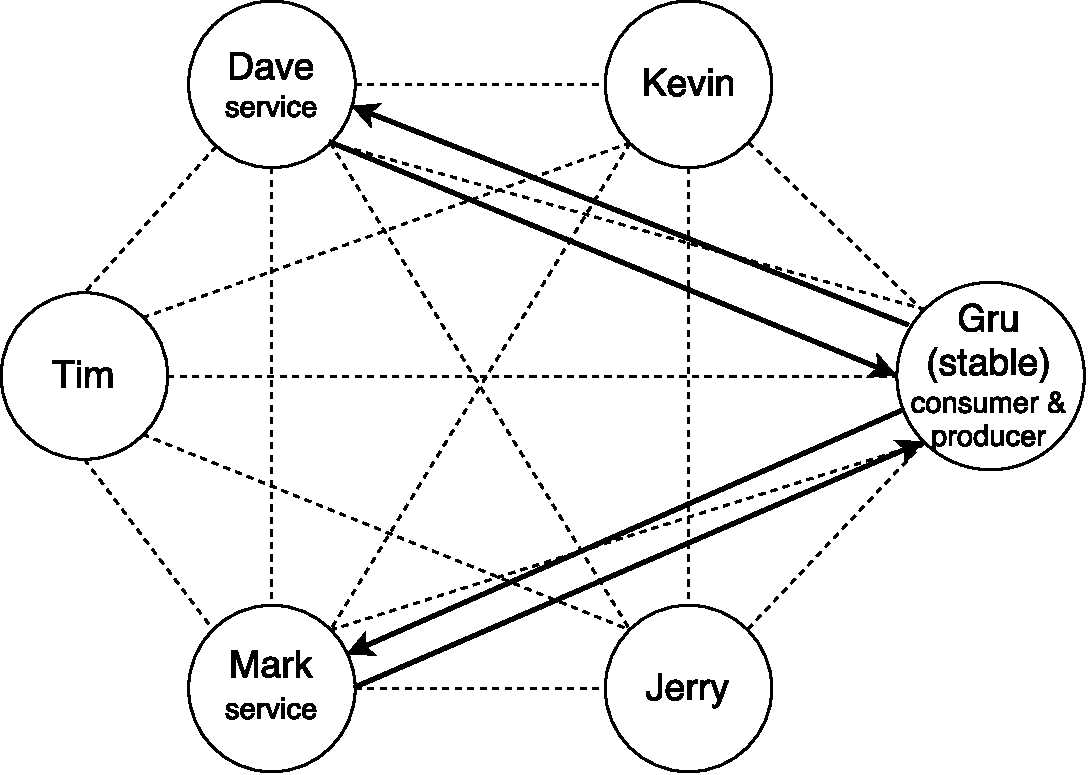
\includegraphics[scale=0.5]{images/evaluation_application.pdf} 
\caption[Computational environment in experiments]{The computational environment used in the experiments. In this example, there is a producer and consumer on Gru, and two replicas of the service actor located on Dave and Mark.} \label{fig:evaluation_application}
\end{figure}

\section{Experiments}
In~\cref{sec:eval_time_t,sec:eval_rel_level,sec:eval_opt,sec:eval_adaptive_rel_model,sec:eval_energy_efficient,sec:eval_replaceable_model} the replication time used by the model, $t_R$ was logged. Recall that the model calculates and uses the 95th percentile value, see~\cref{sec:replication_time}.

\subsection{Measurement of time $t_R$} \label[exp]{sec:eval_time_t}
As mentioned in~\cref{sec:design_time_t}, the time $t$ is the time it takes from that a node on which a replica is running dies, until a new replica is operational. It depends on the time it takes to detect that the node died, and the time it takes to create a new replica. 

The time for detecting that a node has died, $t_d$, was as described in~\cref{sec:node_failure_detection_time} static and set to the upper bound $t_{timeout}$, which in the experiments were 0.5 seconds. While $t_d$ is static, the time for the replication request, $t_R$, varies. In order to model the variation correctly, an experiment was conducted where times were registered and later used to find the best fitting distribution.

The experiment was conducted in two settings. In both settings, two runtimes were started on each of the non-stable servers. In the first experiment, each runtime was given a \emph{MTBF} of 30 seconds, and in the other a \emph{MTBF} of 10 seconds. Furthermore, the required reliability was in the first experiment set to 0.999999, and 0.99995 in the second. Each time $t_R$ was then registered for the duration of the experiment.

The experiment was conducted in two settings with varying failure rates since with higher failure rate, there is a higher risk of the node handling the lost node dies before it finishes, or a node dies before the replication is finished, as described in~\cref{sec:replication_time}. With more stable nodes, i.e. higher \emph{MTBF}, there is a lower risk of this happening. Therefore, the replication times are likely to have less variation in this case. The goal was to find the distribution, among those tested, which best fitted the two data-sets.

\subsubsection*{Results}
The first experiment ran for 230 minutes, and 2000 times were registered, and the second experiment ran for 80 minutes, and 2000 times were registered.

The distributions tested were \emph{beta}, \emph{birnbaumsaunders}, \emph{exponential}, \emph{extreme value}, \emph{gamma generalized pareto}, \emph{inversegaussian}, \emph{logistic}, \emph{logalogistic}, \emph{lognormal}, \emph{nakagami}, \emph{normal}, \emph{rayleigh}, \emph{rician}, \emph{tlocationscale}, \emph{weibull}. Matlab was used to determine which distribution best fitted the data, and the Bayesian information criterion was used to determine how good of a fit a distribution was.

\Cref{fig:distribution_results_30} shows the four best fitted distributions for the first experiment, with nodes' \emph{MTBF} set to 30 seconds, and \cref{fig:distribution_results_10} shows the four best fitted distributions for the second experiment. The figures only show registered values less than 500 ms, for aesthetic reasons. The average values, and number of values above 100 and 500 ms in both experiments are shown in table~\cref{table:tr}. 

When nodes fail more often, there is a higher probability of nodes failing before it finishes to handle a \emph{lost node} request, or to replicate one of its replicas. As described in~\cref{sec:replication_time}, this results in a higher time $t_R$. This is why the average is higher, and there are more times above 100 ms and above 500 ms, in the experiment with \emph{MTBF} of 10 seconds, than the experiment with \emph{MTBF} of 30 seconds.

The log-logistic distribution was found to best fit both data-sets, and is therefore the one used in our model, as described in~\cref{sec:node_failure_detection_time}.

\begin{figure}[!hbt]
\centering
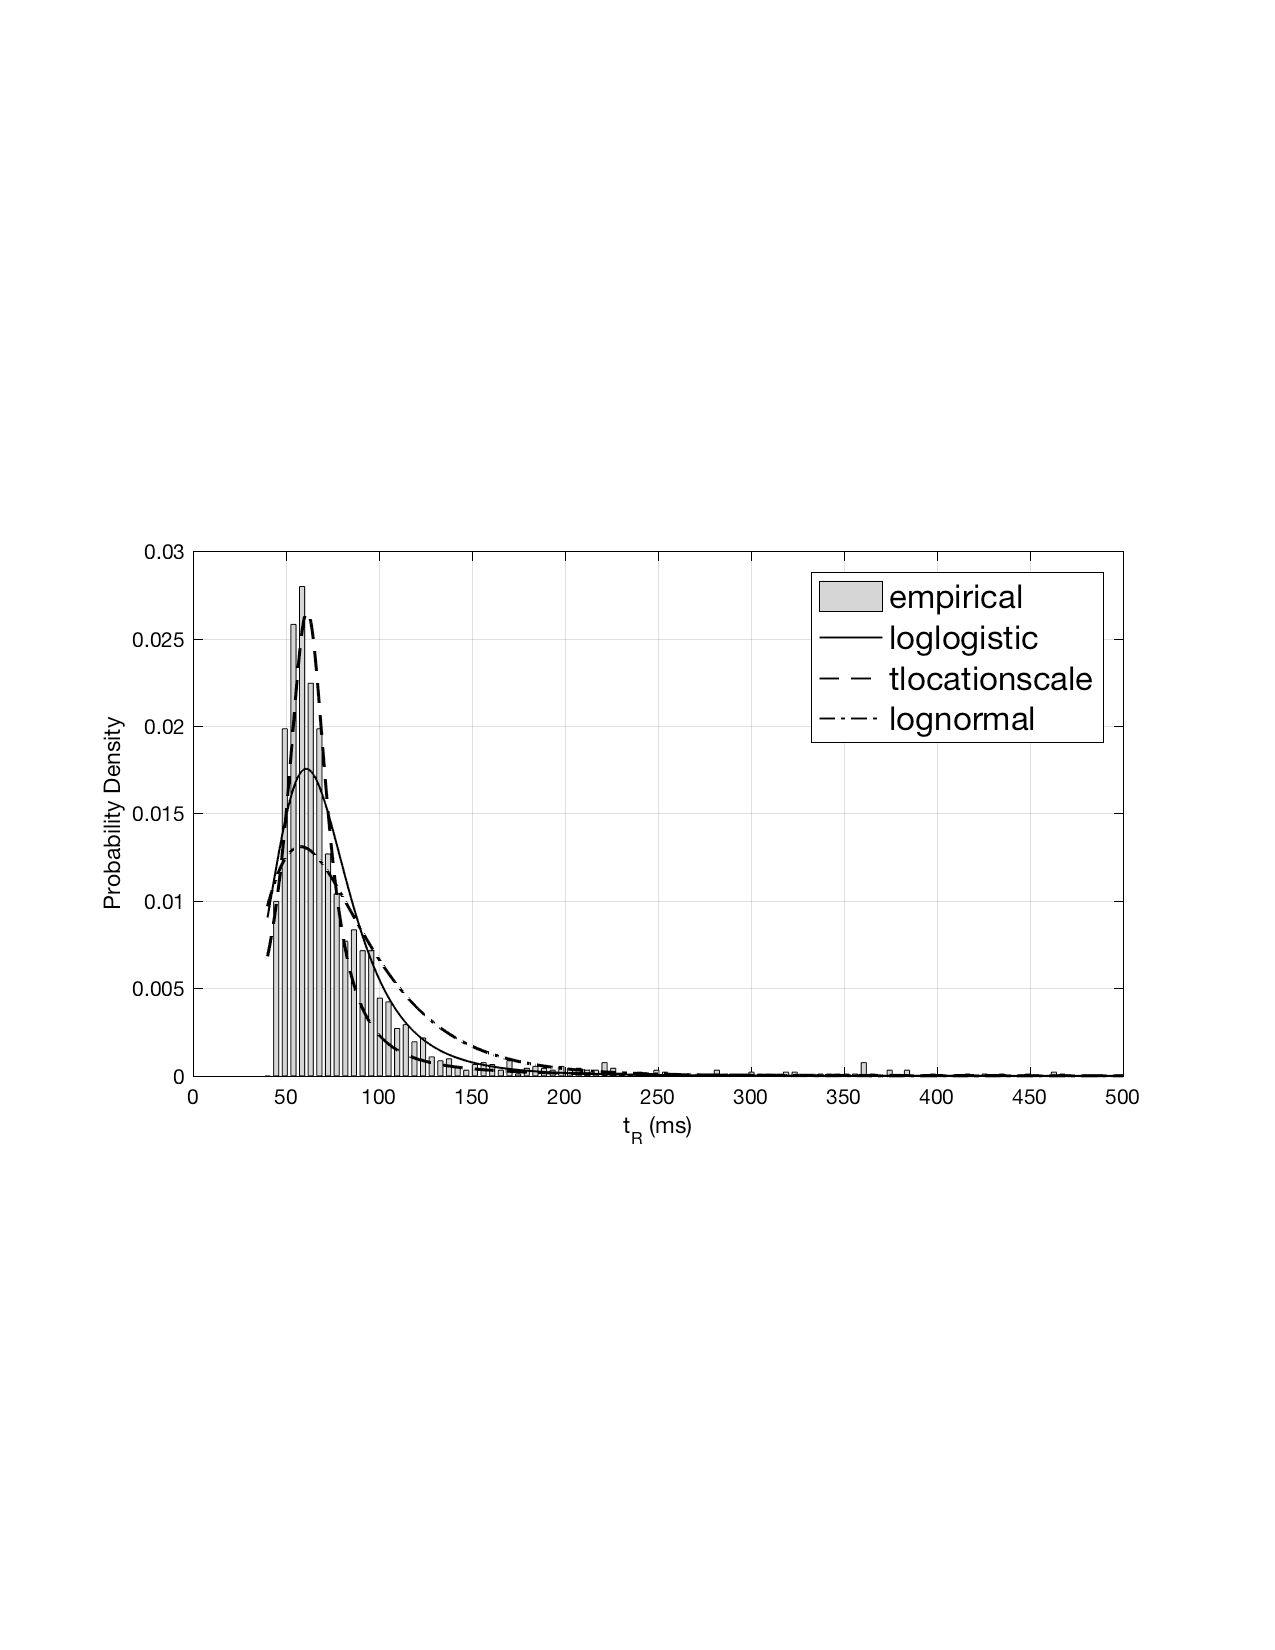
\includegraphics[scale=0.5]{images/results/distribution_results_30.pdf} 
\caption[Fitted distributions in~\cref{sec:eval_time_t}, \emph{MTBF} = 30 s]{Result for~\cref{sec:eval_time_t}. The four best fitted distributions for the failure time data in the first experiment with \emph{MTBF} of nodes set to 30 seconds.}
\label{fig:distribution_results_30}
\end{figure} 

\begin{figure}[!hbt]
\centering
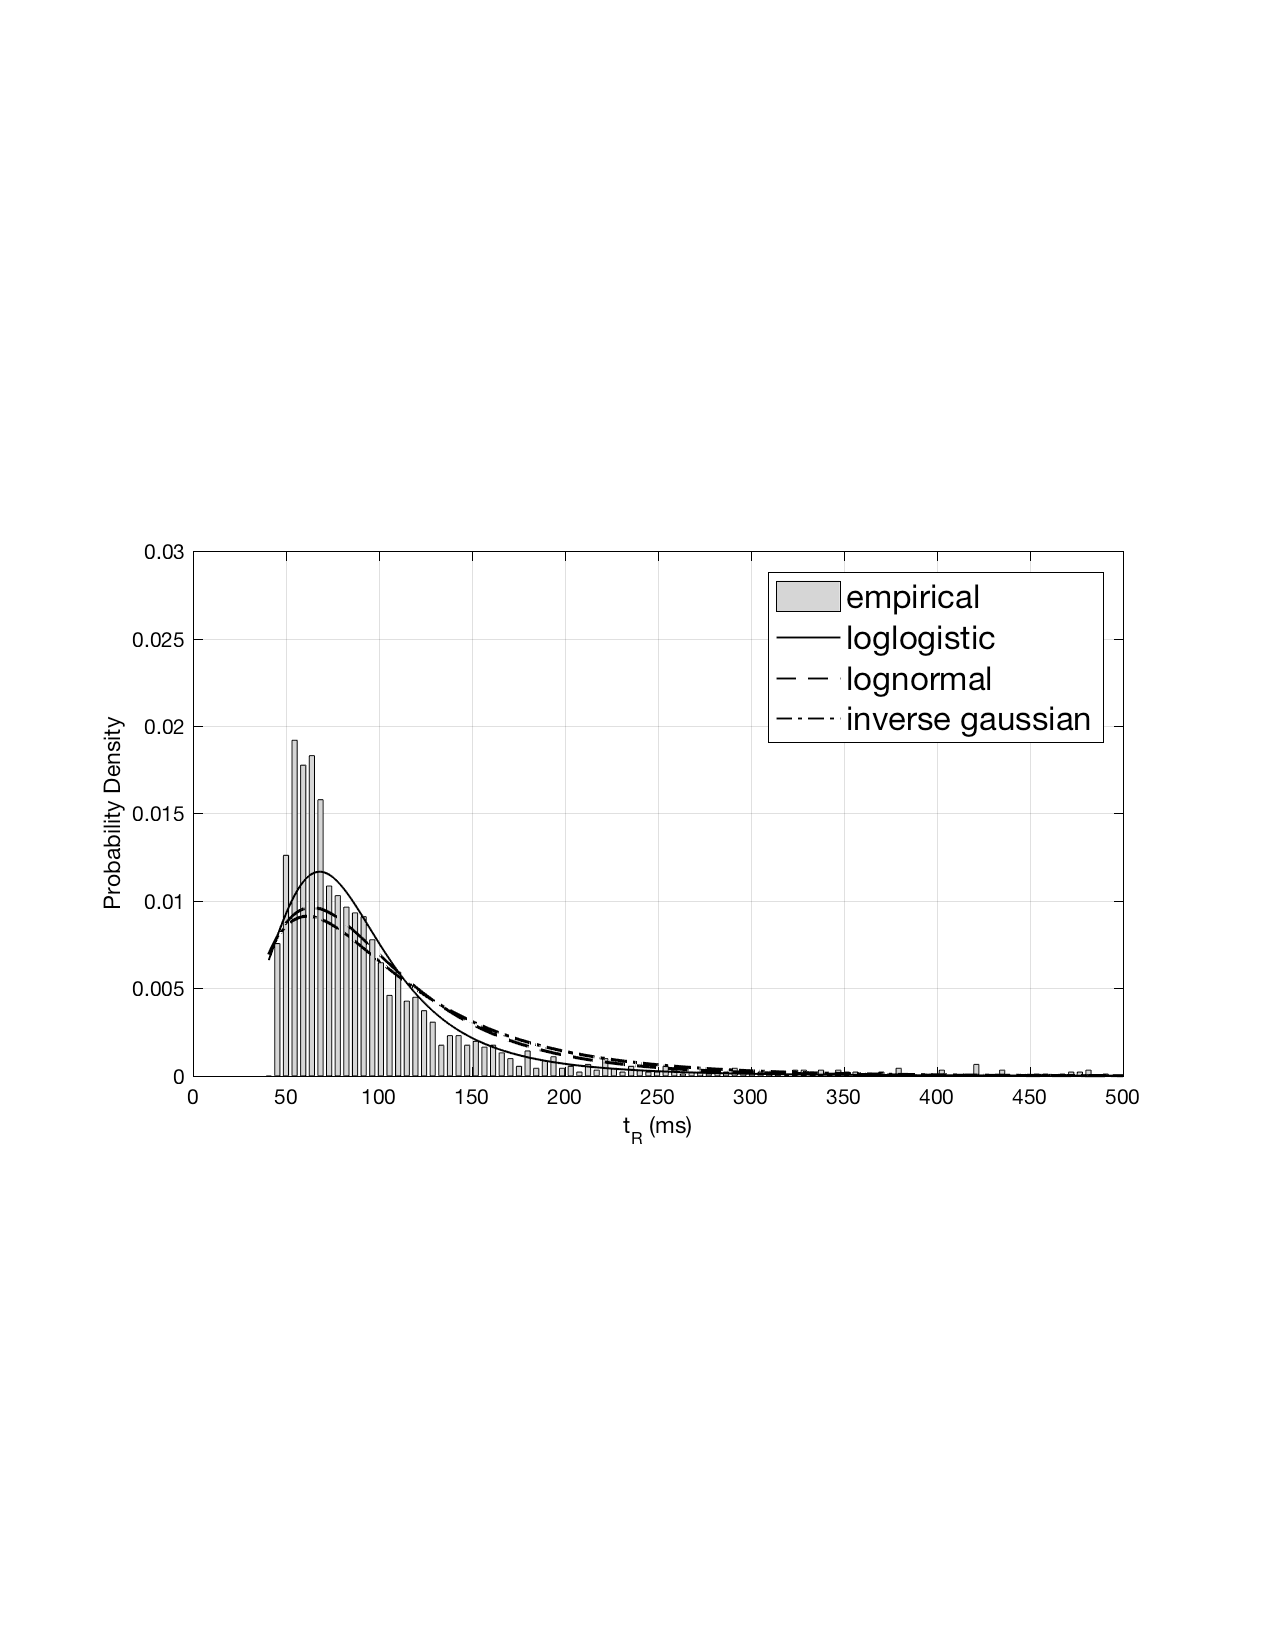
\includegraphics[scale=0.5]{images/results/distribution_results_10.pdf} 
\caption[Fitted distributions in~\cref{sec:eval_time_t}, \emph{MTBF} = 10 s]{Result for~\cref{sec:eval_time_t}. The four best fitted distributions for the failure time data in the second experiment with \emph{MTBF} of nodes set to 10 seconds.} \label{fig:distribution_results_10}
\end{figure}

 \begin{table}[hbt!]
	\begin{center}
	\begin{tabular}{| c | c | c | c | c |}
	 \hline
	 \emph{MTBF} & average & values above 100 ms & values above 500 ms \\
	 \hline
	  30 s & 86.6 & 311 & 15\\
	  10 s & 107.3 & 597 & 34\\
	   \hline
	\end{tabular}
	 \caption[Average $t_R$, number of times above 100 ms and 500 ms in~\cref{sec:eval_time_t}]{Average time $t_R$, number of times above 100 ms, and number of times above 500 ms for \emph{MTBF} 30 and 10 in~\cref{sec:eval_time_t}}
	 \label{table:tr}
	 \end{center}
 \end{table} 

\subsection{Measurement of node failure detection time} \label[exp]{subsec:eval_node_fail_time}
% Is this needed really?
As described in~\cref{sec:design_monitoring}, heartbeats are used to determine whether or not another node is operational. If no heartbeat is received from a node within $t_{timeout}$ seconds (0.5 seconds in the experiments), it is assumed dead. 

In order to measure the time it takes to detect a failed node, an experiment was conducted in which two runtimes were started on the same server. One of the runtimes was periodically killed and restarted. Before killing the runtime, the current time was logged, and on the other node, the time was logged when the node was assumed dead, which in the experiments was 500 ms after the last received heartbeat. The failing node was killed and restarted 1800 times.

\subsubsection*{Results}
The average of the 1800 measured times was 333.5 ms, the minimum was 302.1 ms and the maximum value was 499.8 ms.

All values lie between the theoretical minimum and maximum values of 300 and 500 ms, corresponding to the best and worse case scenarios described in~\cref{sec:node_failure_detection_time}. The average however is clearly below the theoretical average of 400 ms. 
The standard deviation of the times registered was 28.8.
%TODO If higher/lower than theoretical, give a explanation

\subsection{Measurement of replication time $t_r$} \label[exp]{sec:eval_repl_time}
The time it takes to replicate a task, depends on the size of the task state, which have to be sent to the node where the new replica should be created. In Calvin, the state of a task corresponds to the state of the actor representing the task, and consists mainly of the queues of incoming and outgoing data for the actor's in- and out-ports, and any local variables the actor has, as described in~\cref{sec:calvin_actor}.

In the following two experiments, two runtimes were used. The application was first deployed to one of these runtimes, and the service actor was replicated to the other runtime and the time measured. This was repeated for various sizes of the actor's state. The actor had only one out-port and no in-port, and in the first experiment the state of the actor was incrementally increased by increasing the size of a local variable, while in the second experiment the state was increased by increasing the size of its output queue. The state of the actor is only one part of the total replication message. The other part is however static, and its size during the experiment was 349 bytes.
%TODO Is it neccasary or just confusing to mention that the service actor had no inport? 

Both experiments was conducted in two settings. In one, two servers were used with a runtime on each of them, while in the other, a laptop was used on which both the two runtimes were started. The specification of the servers and the laptop are found in~\cref{sec:server_spec} and~\cref{sec:laptop_spec}. For each state size, the actor was replicated 10 times and the times measured.

While measuring the total time, $t_r$, several other times was measured along the way, namely the times to serialize the state, send the state to the other runtime, de-serialize it, create and start the new actor, and send the reply, corresponding to the times described in~\cref{eq:replication_time}.

When the replication was done between runtimes on the same laptop, and the queue size increased, the times were only measured for state sizes less than or equal to 400 MB. This was due to the replication taking too long time. For a state size of 400 MB, each replication took nearly two hours, as shown below, and during the time of the experiment the laptop could not be used, not to affect the results.

For three state sizes, 1, 50 and 100 MB, we measured the replication time 100 times and calculated the standard deviation of these values.

The goal of the experiment was to see how the replication time vary depending on the state size, in which part of the replication process most time is spent, and finally how the replication times varied.

\subsubsection*{Results - total replication time}
\Cref{fig:replication_time_server} and \cref{fig:replication_time_laptop} show how the total replication time vary depending on the state size when replicating between runtimes on different servers, and between runtimes on the same laptop respectively. As shown, the replication time is exponential, and the replication time was higher when increasing the queue size than when increasing the variable size. This is due to the extra time needed when creating the new actor, since then all values in the queue has to be decoded. %TODO decoded?

As seen in~\cref{fig:replication_time_laptop}, when replicating using the laptop, there is a big increase in time when, by increasing the queue, increasing the state size from 200 MB to 400 MB. This is due to running out of memory, and the process started using the system's SWAP memory, which significantly reduced the performance. 

\begin{figure}[hbt!]
\centering
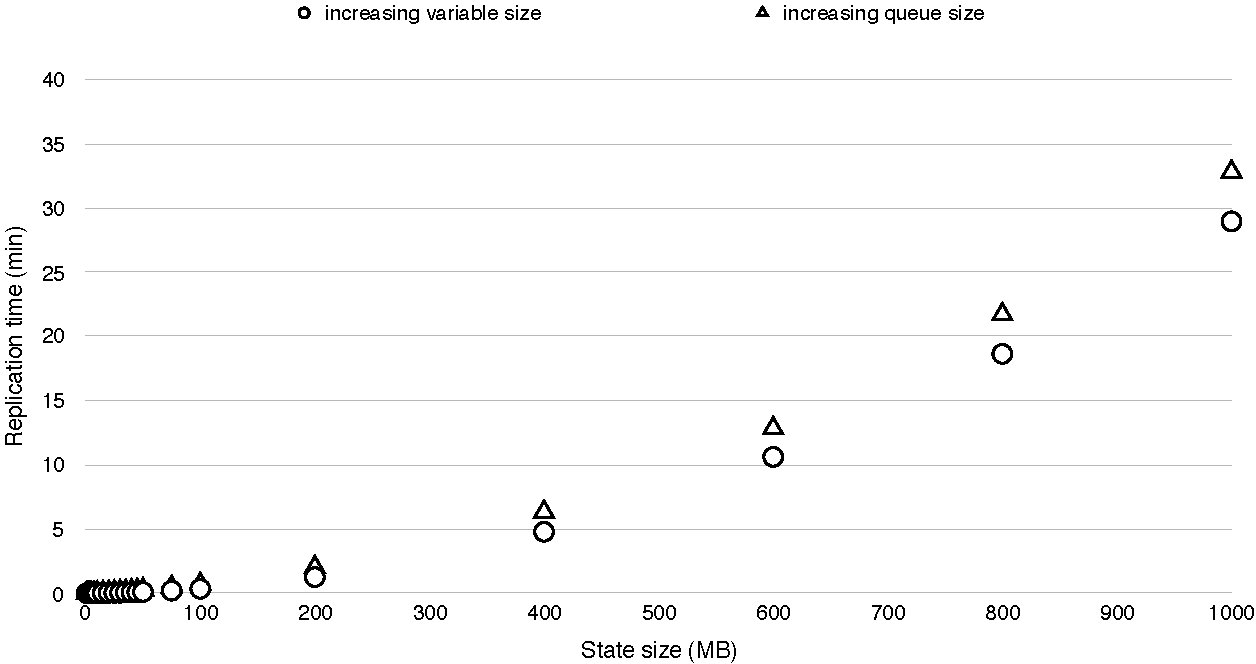
\includegraphics[scale=0.5]{images/results/replication_time/server.pdf} 
\caption[Replication time in~\cref{sec:eval_repl_time}, server-server]{Result for~\cref{sec:eval_repl_time}. The average replication time as a function of state size, where the state size was increased by increasing the size of one of the actor's variables, and the replication was done between two runtimes on different servers.} \label{fig:replication_time_server}
\end{figure}

\begin{figure}[hbt!]
\centering
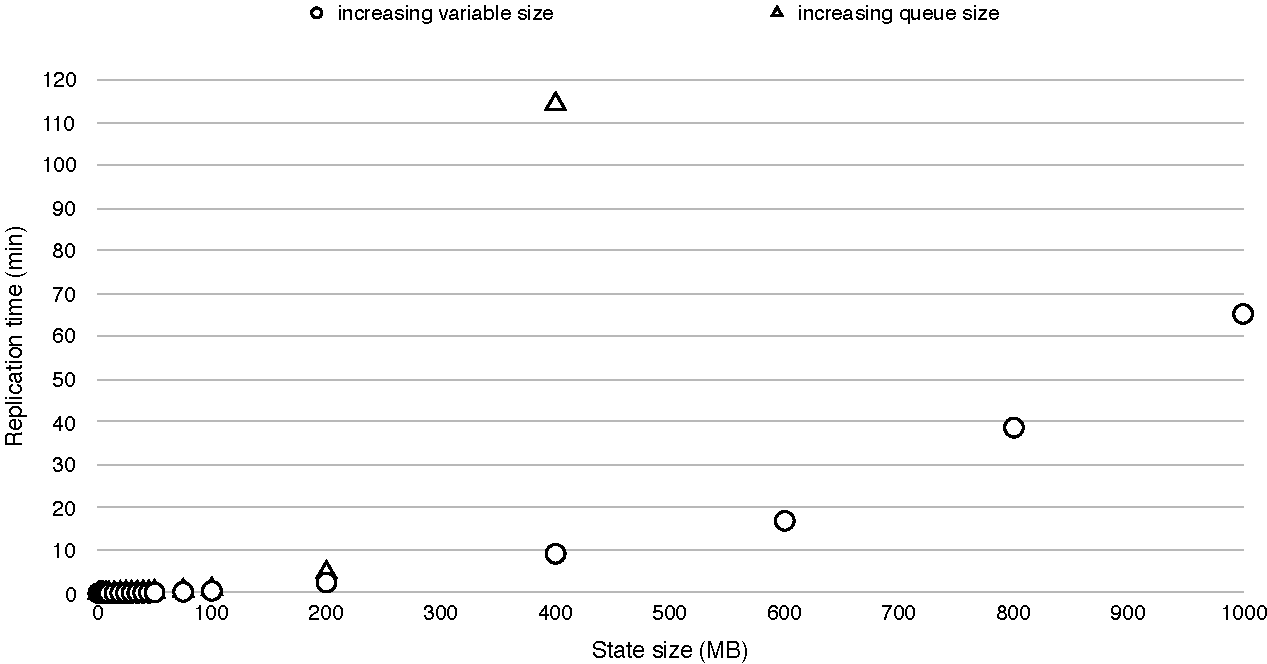
\includegraphics[scale=0.5]{images/results/replication_time/laptop.pdf} 
\caption[Replication time in~\cref{sec:eval_repl_time}, laptop-laptop]{Result for~\cref{sec:eval_repl_time}. The average replication time as a function of state size, where the state size was increased by increasing the size of the actor's port queue, and the replication was done between two runtimes on the same laptop.} \label{fig:replication_time_laptop}
\end{figure}

\subsubsection*{Results - replication time parts}
\Cref{fig:replication_time_parts_server_variable} and \cref{fig:replication_time_parts_server_queue} show how much of the total replication time was spent on the various parts of the replication process when increasing the variable size and queue size respectively, and when replicating between the two servers. As shown, the time to create the new replica takes significantly larger part of the total time when increasing the queue size rather than the variable size. This is due to the time spent on decoding the queue's values as described above.

Furthermore, significantly more time was spent on transmitting the state to the other node as the state size was increased. Hence for large state sizes, the total replication time depends mostly on the bandwidth of the links connecting the various nodes. For smaller state sizes, the replication time is more CPU bound, especially when increasing the queue size.

%TODO needs work.
\Cref{fig:replication_time_parts_laptop_variable} and \cref{fig:replication_time_parts_laptop_queue} show how much of the total replication time was spent on the various parts of the replication process, when increasing the variable size and queue size respectively, and when the replication was done between two runtimes on the same laptop. Again, more time is spent on creating the new actor when increasing the queue size than when increasing the variable size. %Might result in that actor blocking the others in the scheduling loop

Furthermore, the time spent on transmitting the state increases when increasing the state size. However, as shown in~\cref{fig:replication_time_parts_laptop_queue}, when replicating from laptop to laptop an actor with state size above 100 MB (when increasing the queue size), more time was spent on creating the actor. This, as described before, is due to running out of memory. In the experiment, this happened when the size was 200 MB or more, and when this happens, the process needs to use the system's swap memory when creating the new actor. The laptops 1333 MHz ram memory has a speed of approximately 21 GB/s, which compared to the SSD speed of 540 MB/s explains the significantly drop in performance.

\begin{figure}[hbt!]
\centering
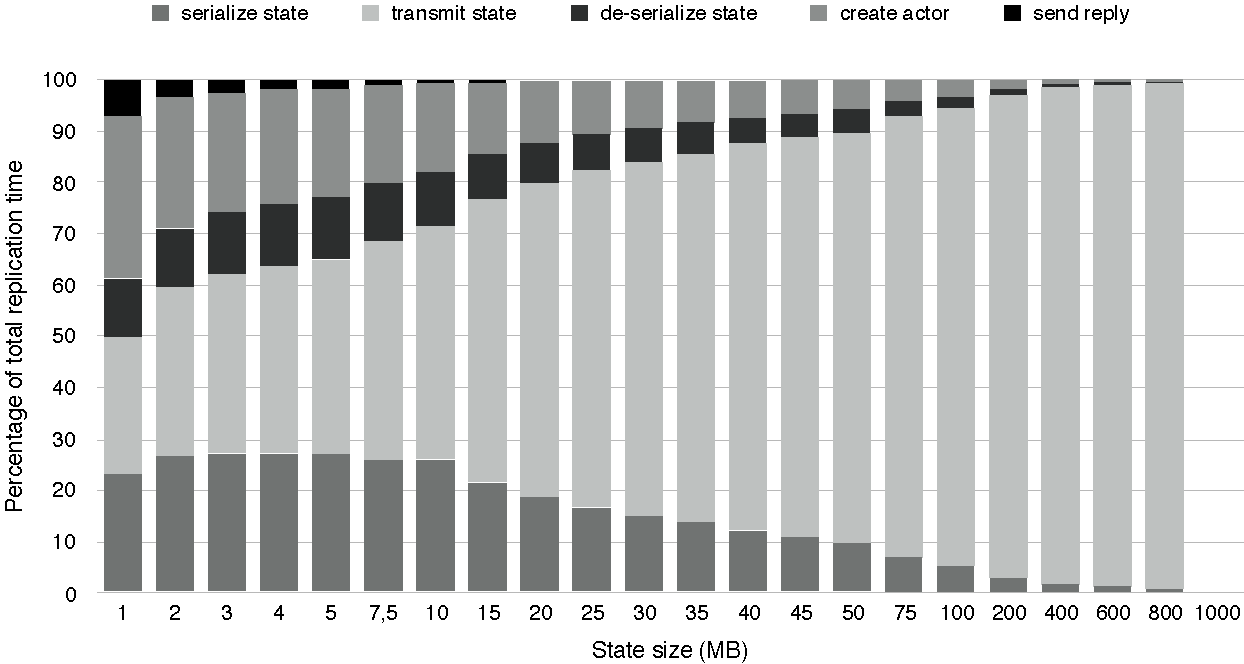
\includegraphics[scale=0.5]{images/results/replication_time/server_parts_variable.pdf} 
\caption[Replication time parts in~\cref{sec:eval_repl_time}, server-server, increasing variable size]{Result for~\cref{sec:eval_repl_time}. Time, of the total replication time, spent on the different parts of the replication, when replicating from server to server, and increasing the size of one of the actor's variables.} \label{fig:replication_time_parts_server_variable}
\end{figure}

\begin{figure}[hbt!]
\centering
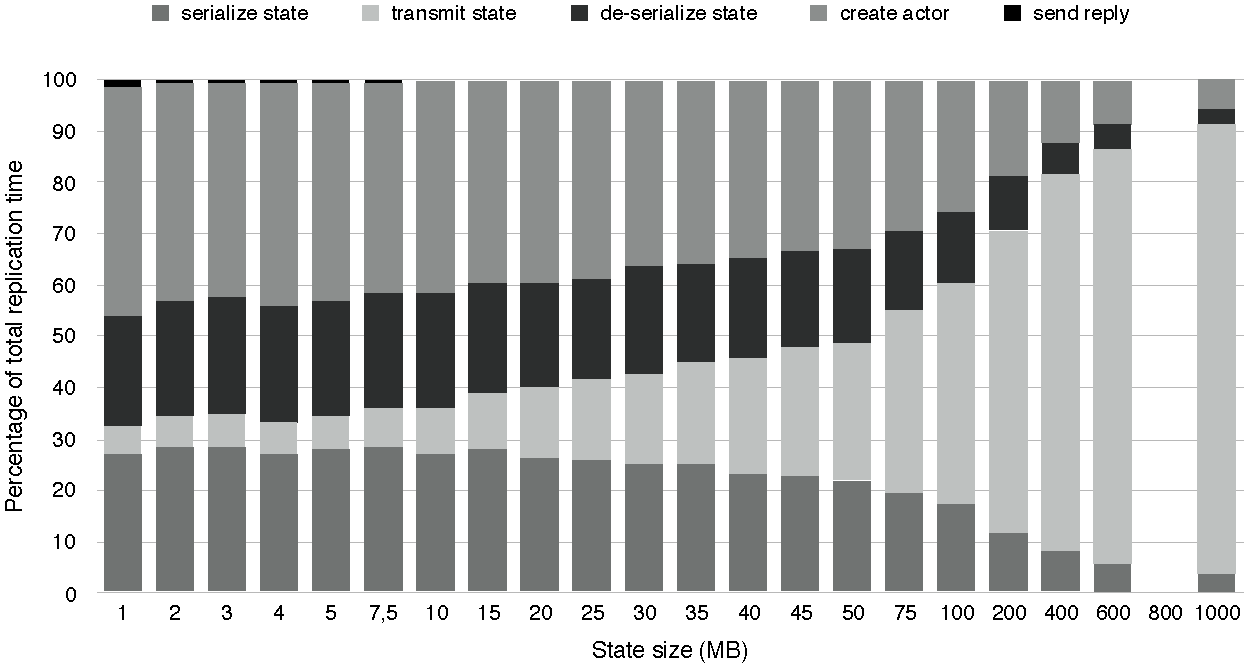
\includegraphics[scale=0.5]{images/results/replication_time/server_parts_queue.pdf} 
\caption[Replication time parts in~\cref{sec:eval_repl_time}, server-server, increasing queue size]{Result for~\cref{sec:eval_repl_time}. Time, of the total replication time, spent on the different parts of the replication, when replicating from server to server, and increasing the size of the actor's port queue.} \label{fig:replication_time_parts_server_queue}
\end{figure}

\begin{figure}[hbt!]
\centering
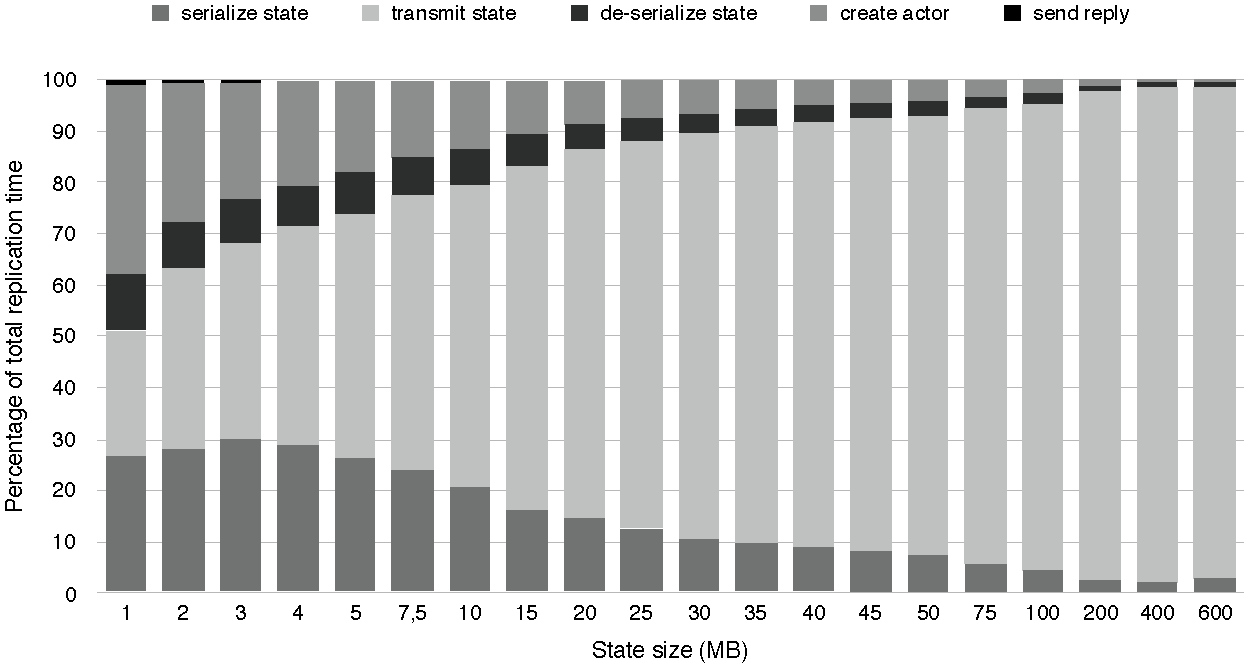
\includegraphics[scale=0.5]{images/results/replication_time/laptop_parts_variable.pdf} 
\caption[Replication time parts in~\cref{sec:eval_repl_time}, laptop-laptop, increasing variable size]{Result for~\cref{sec:eval_repl_time}. Time, of the total replication time, spent on the different parts of the replication, when replicating from laptop to laptop, and increasing the size of one of the actor's variables.} \label{fig:replication_time_parts_laptop_variable}
\end{figure}

\begin{figure}[hbt!]
\centering
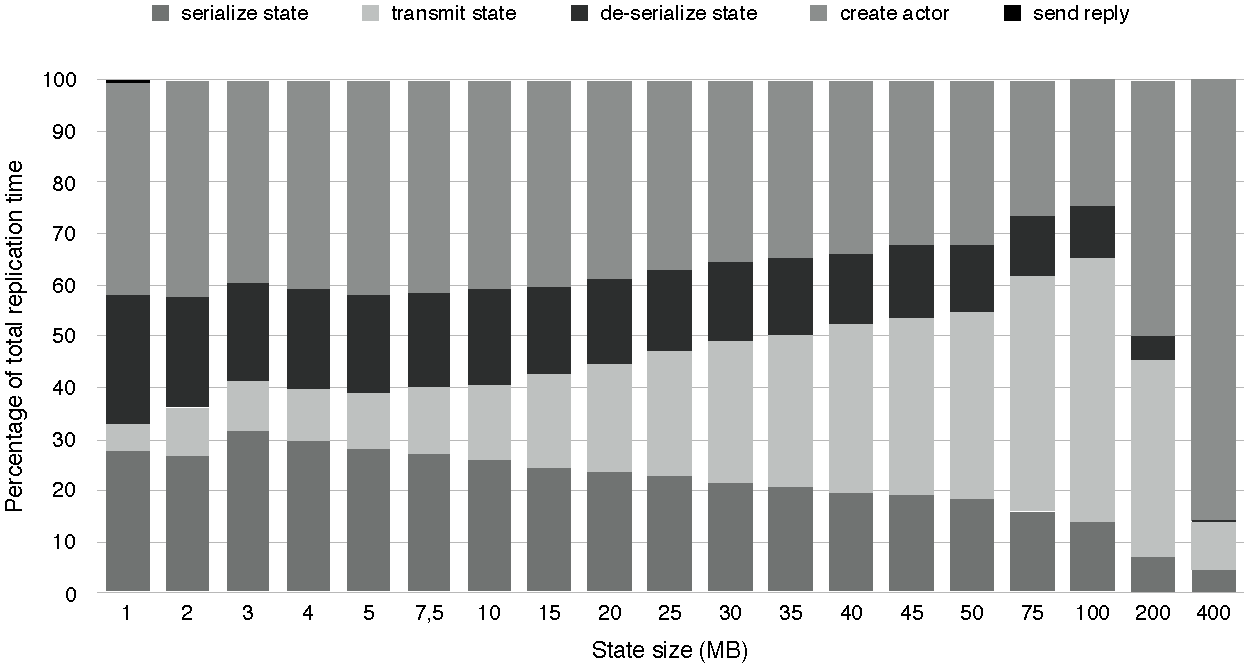
\includegraphics[scale=0.5]{images/results/replication_time/laptop_parts_queue.pdf} 
\caption[Replication time parts in~\cref{sec:eval_repl_time}, laptop-laptop, increasing queue size]{Result for~\cref{sec:eval_repl_time}. Time, of the total replication time, spent on the different parts of the replication, when replicating from laptop to laptop, and increasing the size of the actor's port queue.} \label{fig:replication_time_parts_laptop_queue}
\end{figure}

\subsubsection*{Results - replication time variance}
For 1, 50 and 100 MB the replication time was measured 100 times. The variance of the replication times was very small. \Cref{table:replication_time_variation_variable} and \cref{table:replication_time_variation_queue} show the average replication time ($\mu$), the standard deviation ($\sigma$), and the relative standard deviation (RSD), calculated as $\frac{\sigma}{\mu}$, for these three state sizes when increasing the variable's size, and the size of the queue respectively. The variance was as shown very low. 

However, in a real setting, the replication time will vary depending on the state of the system. When increasing the queue size, the replication time is more CPU bound than when increasing the size of a variable, and therefore the replication time is dependent on the current load of the two nodes. Furthermore, for larger state sizes when the transmission time is the largest part of the replication time, the total time will vary depending on the network load of the system.
 
 \begin{table}[h!]
	\begin{center}
	\begin{tabular}{| c | c | c | c | c |}
	 \hline
	 replicating from/to & state size (MB) & $\mu$ (s) & $\sigma$ (s) & RSD \\
	 \hline		%TODO values
	  server/server & 1 & 0.041 & 0.001 & 0.024 \\
	  server/server & 50 &  5.523 &  0.056 & 0.010 \\
	  server/server & 100 &  20.177 & 0.385 & 0.019 \\
	  laptop/laptop & 1 & 0.087 & 0.020 & 0.229 \\
	  laptop/laptop & 50 & 10.617 & 1.210 & 0.114 \\
	  laptop/laptop & 100 & 34.019 & 1.412 & 0.041 \\
	   \hline
	\end{tabular}
	 \caption[Average replication time, standard deviation and RSD in~\cref{sec:eval_repl_time}, increased variable size]{Result for~\cref{sec:eval_repl_time}. Average replication time ($\mu$), standard deviation ($\sigma$), and the relative standard deviation (RSD), for state sizes 1, 50 and 100 MB, where the state size was increased by increasing the size of one of the actor's variables.}
	 \label{table:replication_time_variation_variable}
	 \end{center}
 \end{table}
 
\begin{table}[h!]
	\begin{center}
	\begin{tabular}{| c | c | c | c | c |}
	 \hline
	 replicating from/to & state size (MB) & $\mu$ (s) & $\sigma$ (s) & RSD \\
	 \hline		%TODO values
	  server/server & 1 & 0.251 & 0,008 & 0,032 \\
	  server/server & 50 & 16,547 & 0.256 & 0,015 \\
	  server/server & 100 & 42.555 & 0.414 & 0,010 \\
	  laptop/laptop & 1 & 0.348 & 0.043 & 0.124 \\
	  laptop/laptop & 50 & 19.075 & 0.299 & 0.016 \\
	  laptop/laptop & 100 & 50.893 & 1.066 & 0.021 \\
	   \hline
	\end{tabular}
	 \caption[Average replication time, standard deviation and RSD in~\cref{sec:eval_repl_time}, increased queue size]{Result for~\cref{sec:eval_repl_time}. Average replication time ($\mu$), standard deviation ($\sigma$), and the relative standard deviation (RSD), for state sizes 1, 50 and 100 MB, where the state size was increased by increasing the size of the actor's port queue.}
	 \label{table:replication_time_variation_queue}
	 \end{center}
 \end{table}
 

\subsection{Ensuring a certain reliability level} \label[exp]{sec:eval_rel_level}
In this experiment, two runtimes were started on each of the unstable servers. Each runtime was given a \emph{MTBF} of 20 seconds.

After the application was started, the reliability level of the nodes on which replicas were running was periodically measured. The required reliability was set to 0.98.

The experiment was considered successful if the momentary reliability, when dropped below the required, was restored to a level above the required. 

\subsubsection*{Results}
The experiment ran for 5 minutes, and \cref{fig:exp_reliability_level} shows how the reliability vary during this period. The average reliability for the duration of the whole experiment was 0.996, clearly above the required level of 0.98. The average of the 95th percentile values for the replication time, $t_R$ was during the experiment 583,9 ms.

As shown in the figure, the reliability was lower in the beginning of the experiment. This is due the lack of failure data for nodes, therefore assuming the default value for the \emph{MTBF} of 10 seconds. As the nodes starts failing, the system learns their actual \emph{MTBF}, which in the experiment was 20 seconds. Every drop in reliability corresponds to a failure of one of the nodes on which a replica is executing. The experiment shows clearly that the momentary reliability level is restored to a level above the required level and the experiment if therefore considered successful.

%TODO this needs to be updated? Not the latest?
\begin{figure}[!hbt]
\centering
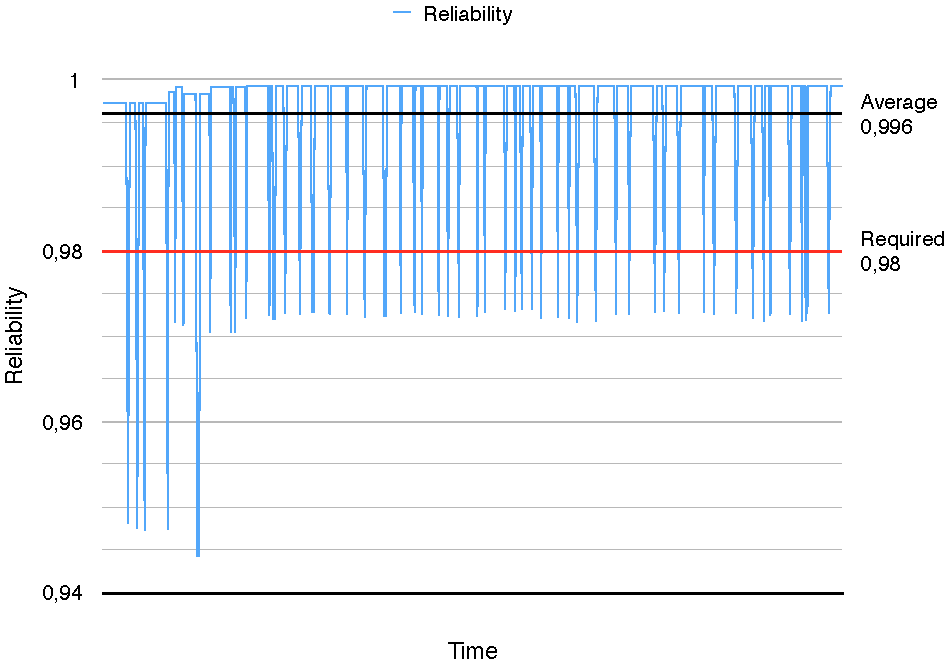
\includegraphics[scale=0.5]{images/results/reliability.pdf}
\caption[Reliability over time in~\cref{sec:eval_rel_level}]{Result for~\cref{sec:eval_rel_level}. Reliability over time in a system with failing nodes.} \label{fig:exp_reliability_level}
\end{figure}

\subsection{Optimal number of replicas} \label[exp]{sec:eval_opt}
\subsubsection{Choosing the most reliable} \label[exp]{sec:eval_opt_nbr_replicas}
In this experiment, the two runtimes were started on each of the unstable servers. The \emph{MTBF} for the various runtimes varied. The mean values given to the different nodes are presented in \cref{table:exp_nodes_means}.

\begin{table}[h]
	\begin{center}
	\begin{tabular}{| c | c |}
	 \hline
	 node & \emph{MTBF} (s) \\
	 \hline		
	  $dave_1$ & 7.5 \\
	  $dave_2$ & 7.5 \\
	  $tim_1$ & 7.5 \\
	  $tim_2$ & 7.5 \\
	  $kevin_1$ & 15 \\
	  $kevin_2$ & 15 \\
	  $mark_1$ & 15 \\
	  $mark_2$ & 40 \\
	  $jerry_1$ & 40 \\
	  $jerry_2$ & 40 \\
	   \hline
	\end{tabular}
	 \caption[\emph{MTBF} for nodes in~\cref{sec:eval_opt_nbr_replicas}]{Mean-time-between-failures for the ten unstable runtimes in~\cref{sec:eval_opt_nbr_replicas}.}
	 \label{table:exp_nodes_means}
	 \end{center}
 \end{table}

After the application was started, the reliability level of the nodes on which replicas were running was periodically measured. The required level of reliability was set to 0.999.

The experiment was considered successful if, as the system learned the actual \emph{MTBF} for the nodes, the system placed the replicas on the most reliable nodes. Furthermore, for the experiment to be considered successful, the momentary reliability should lie above the required, and if below it should be restored to a level above the required.

\subsubsection*{Results}
The experiment ran for 5 minutes, and~\cref{fig:exp_opt_replicas_total} shows the number of replicas over time, while~\cref{fig:exp_opt_replicas_MTBF_30,fig:exp_opt_replicas_MTBF_15,fig:exp_opt_replicas_MTBF_75} show the number of replicas for each of the unstable nodes over time.

The average of the 95th percentile values for the replication time, $t_R$ was during the experiment 599,1 ms.

As shown in the figures, the number of replicas decreased over time, from three replicas at the start of the experiment, to later only two. This is due to the system learning the nodes' \emph{MTBF} and thereafter placing the replicas on the more reliable ones. This is shown in \cref{fig:exp_opt_replicas_MTBF_30,fig:exp_opt_replicas_MTBF_15,fig:exp_opt_replicas_MTBF_75}, where the number of replicas per node is shown. It is clear that the more reliable nodes, $mark_2$, $jerry_1$, and $jerry_2$, were chosen more often than the less reliable ones. The experiment was therefore considered successful.

\begin{figure}[!hbt]
\centering
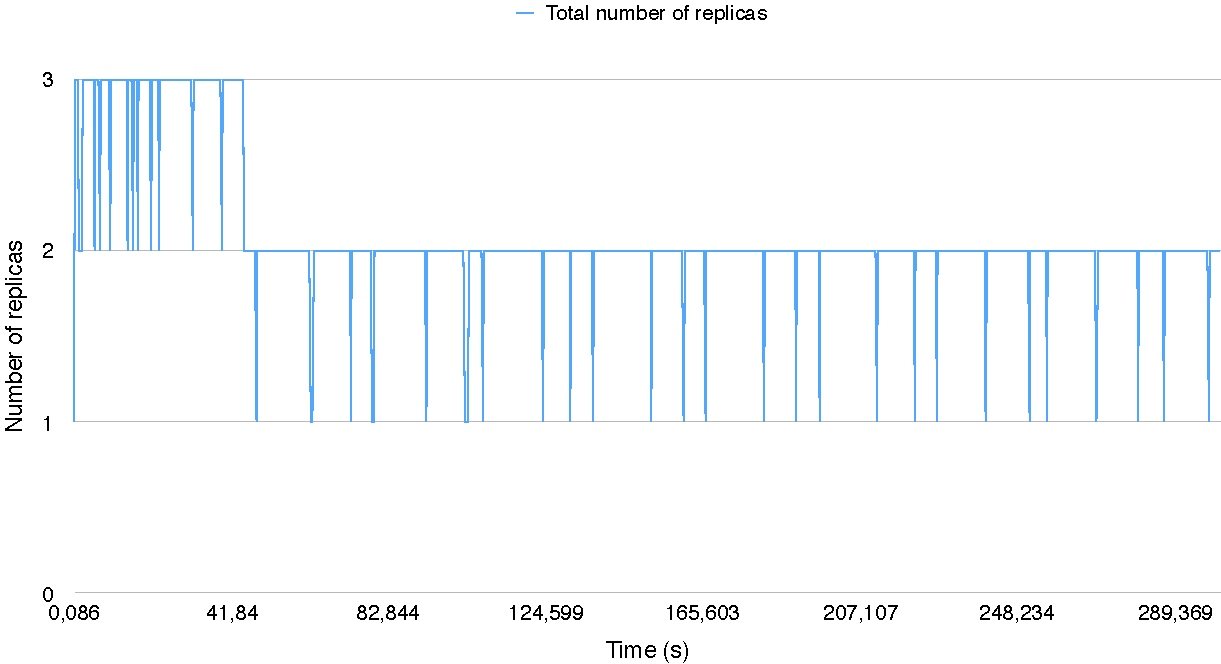
\includegraphics[scale=0.5]{images/results/optimal_replicas/total.pdf}
\caption[Total number of replicas in~\cref{sec:eval_opt_nbr_replicas}]{Result for~\cref{sec:eval_opt_nbr_replicas}. Total number of replicas.} \label{fig:exp_opt_replicas_total}
\end{figure}

\begin{figure}[!hbt]
\centering
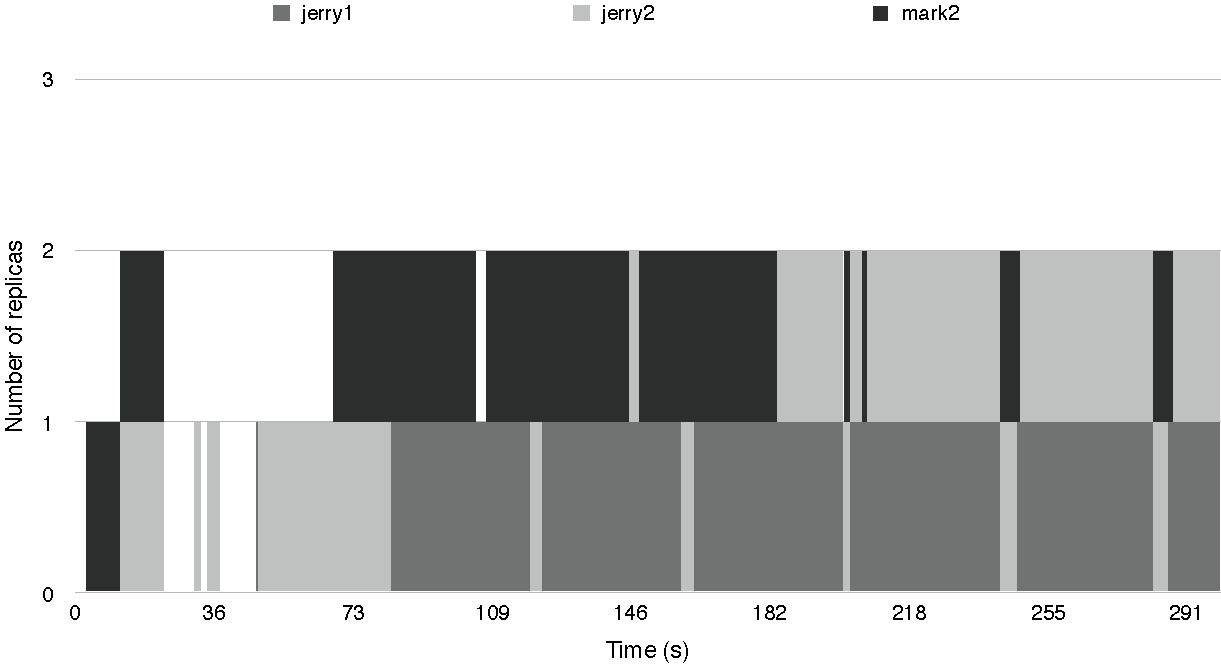
\includegraphics[scale=0.5]{images/results/optimal_replicas/MTBF_30.pdf}
\caption[Number of replicas in~\cref{sec:eval_opt_nbr_replicas} on nodes with \emph{MTBF} = 30 s]{Result for~\cref{sec:eval_opt_nbr_replicas}. Number of replicas per node, for the three nodes with a \emph{MTBF} of 30 seconds.} \label{fig:exp_opt_replicas_MTBF_30}
\end{figure}

\begin{figure}[!hbt]
\centering
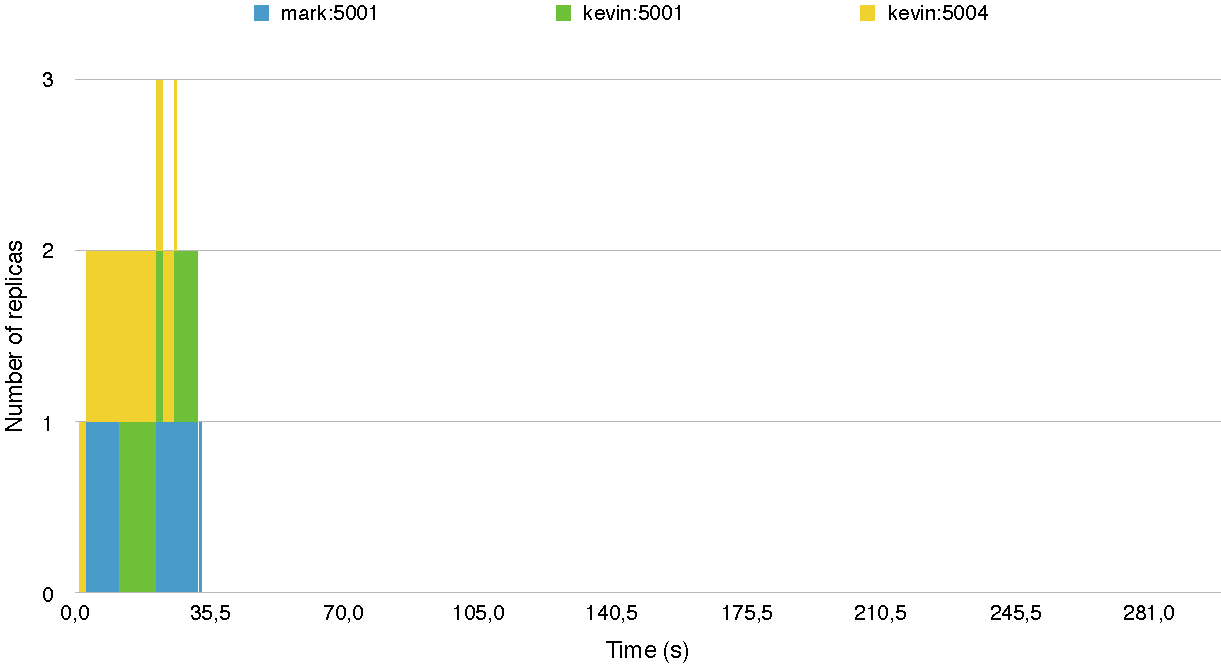
\includegraphics[scale=0.5]{images/results/optimal_replicas/MTBF_15.pdf}
\caption[Number of replicas in~\cref{sec:eval_opt_nbr_replicas} on nodes with \emph{MTBF} = 15 s]{Result for~\cref{sec:eval_opt_nbr_replicas}. Number of replicas per node, for the three nodes with a \emph{MTBF} of 15 seconds.} \label{fig:exp_opt_replicas_MTBF_15}
\end{figure}

\begin{figure}[!hbt]
\centering
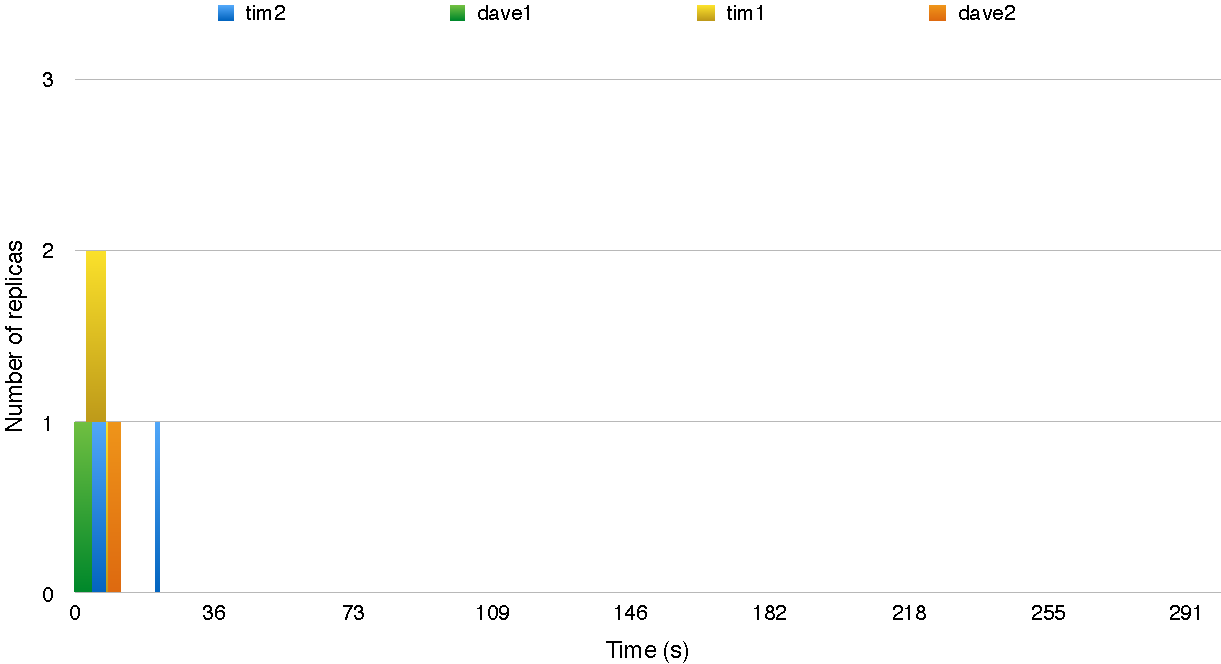
\includegraphics[scale=0.5]{images/results/optimal_replicas/MTBF_75.pdf}
\caption[Number of replicas in~\cref{sec:eval_opt_nbr_replicas} on nodes with \emph{MTBF} = 7.5 s]{Result for~\cref{sec:eval_opt_nbr_replicas}. Number of replicas per node, for the four nodes with a \emph{MTBF} of 7.5 seconds.} \label{fig:exp_opt_replicas_MTBF_75}
\end{figure}

\subsubsection{Optimal replicas} \label[exp]{sec:eval_opt_nbr_replicas_2}
In order to show that the system automatically reduces the number of replicas in case more reliable nodes are available, we conducted an experiment in which five runtimes were started on the unstable servers. Two of these were given a \emph{MTBF} of 25 seconds, while the other three were not killed. Since these three were not killed, they were not actually \emph{unstable}, but the system used the default \emph{MTBF} of 10 seconds for these nodes. Consequently, despite not failing, the system considered them less reliable than the two failing nodes with a \emph{MTBF} of 25 seconds. The reason for not killing those three nodes were simply in order to show that the system automatically minimizes the number of replicas when the optimization algorithm runs, not only when a node fails. The required reliability in the experiment was set to 0.999. Finally, for aesthetic reasons, a delay of 5 seconds were used between killing and restarting nodes \emph{kevin} and \emph{jerry}.

\subsubsection*{Results}
The experiment ran for 5 minutes. As mentioned, the default \emph{MTBF} is 10 seconds when no failure data is known for a node. Therefore, before the reliable nodes, $kevin$ and $jerry$, had failed twice, the system used the default \emph{MTBF} of 10 seconds. After having failed twice, the system could learn their actual \emph{MTBF} of 25 seconds. This is why there is a period during which none of the reliable nodes are given any replicas. After their second failure however, it is known that they are actually more reliable than the other ones, why replicas are then moved to those nodes.

The average of the 95th percentile values for the replication time, $t_R$ was during the experiment 567,7 ms. This resulted in that as long as the two reliable nodes were available, only two replicas were needed, but if one, or both of them died, three replicas were needed to reach the required reliability. This is shown in~\cref{fig:exp_opt_replicas_total_2}, where the total number of replicas are shown. 

\Cref{fig:exp_opt_replicas_MTBF_25_2,fig:exp_opt_replicas_MTBF_10_2} shows the number of replicas per node and it seen that the system moves replicas from the less reliable nodes to the more reliable nodes as soon there is a more reliable node available. The experiment was therefore considered successful.

\begin{figure}[!hbt]
\centering
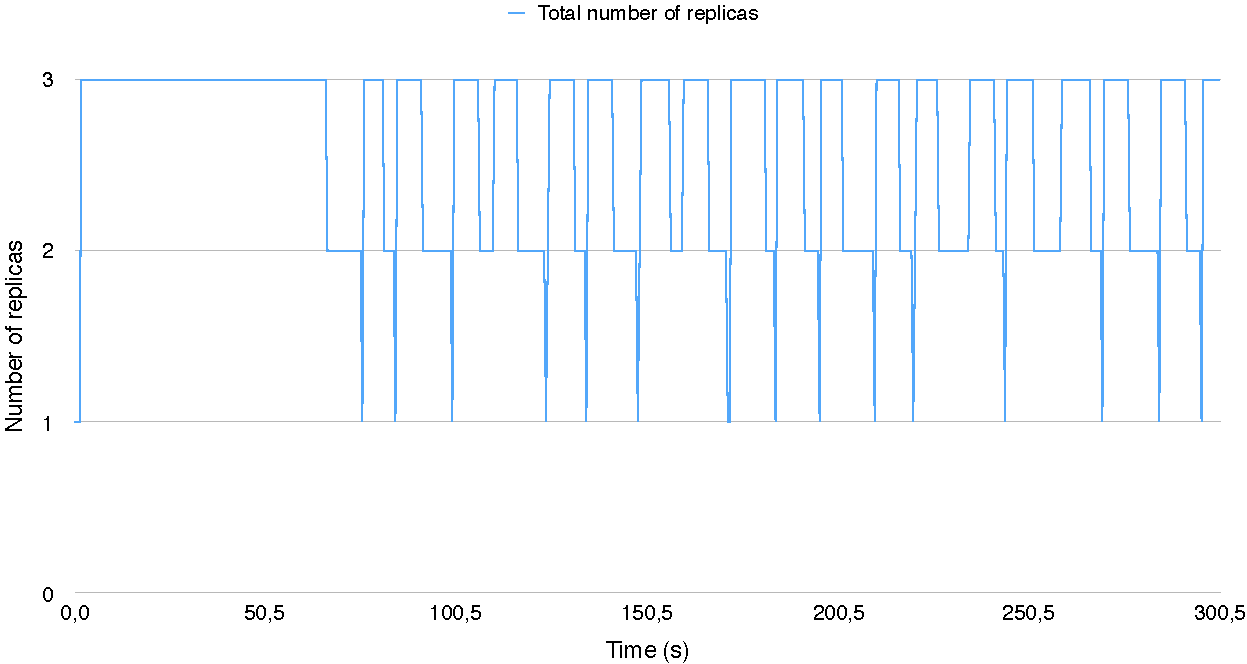
\includegraphics[scale=0.5]{images/results/optimal_replicas/2/total.pdf}
\caption[Total number of replicas in ~\cref{sec:eval_opt_nbr_replicas_2}]{Result for~\cref{sec:eval_opt_nbr_replicas_2}. Total number of replicas.} \label{fig:exp_opt_replicas_total_2}
\end{figure}

\begin{figure}[!hbt]
\centering
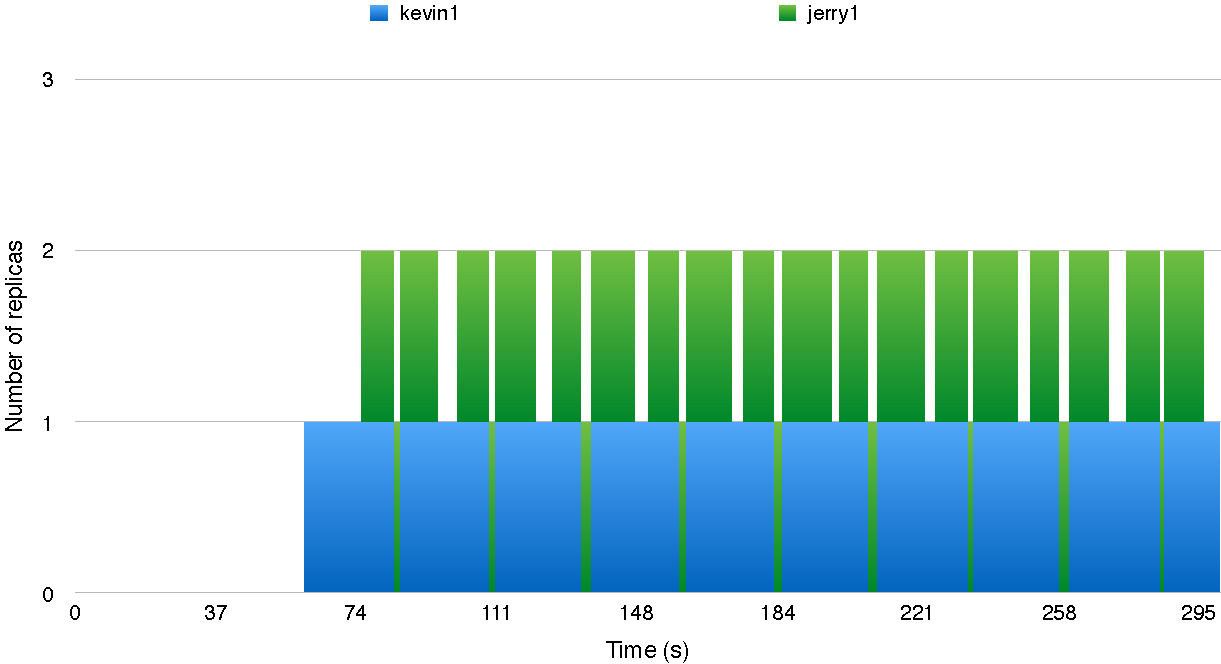
\includegraphics[scale=0.5]{images/results/optimal_replicas/2/MTBF_25.pdf}
\caption[Number of replicas in ~\cref{sec:eval_opt_nbr_replicas_2} on nodes with \emph{MTBF} = 25 s]{Result for~\cref{sec:eval_opt_nbr_replicas_2}. Number of replicas per node, for the two nodes with a \emph{MTBF} of 25 seconds.} \label{fig:exp_opt_replicas_MTBF_25_2}
\end{figure}

\begin{figure}[!hbt]
\centering
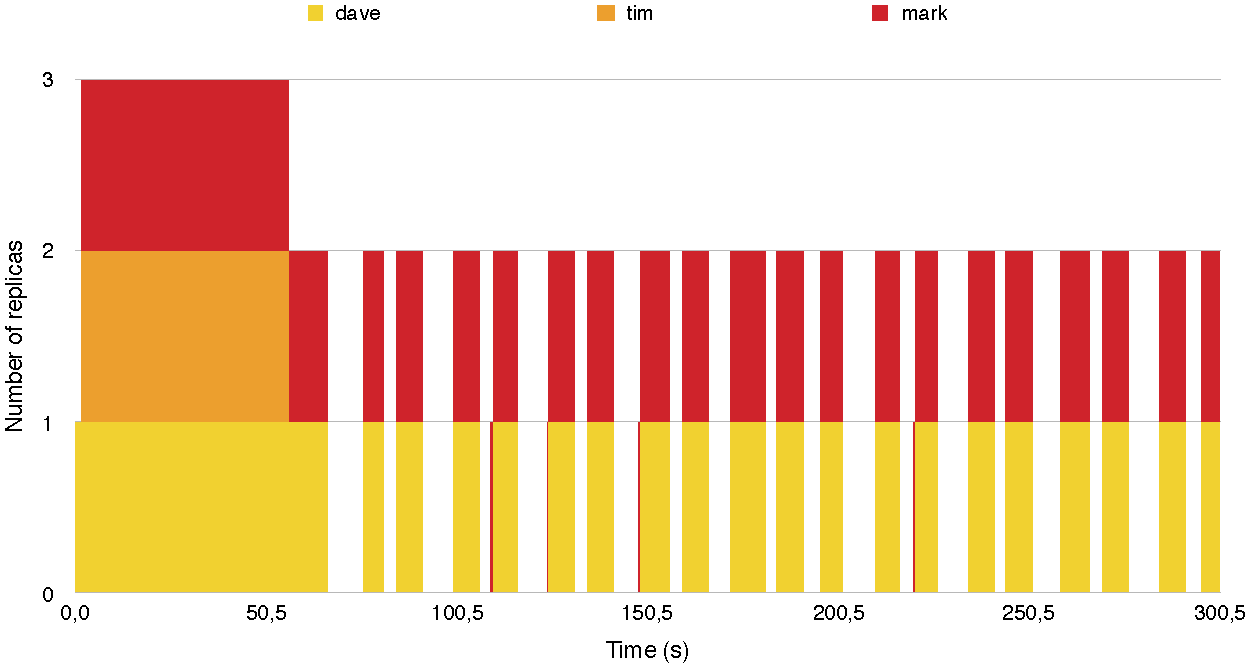
\includegraphics[scale=0.5]{images/results/optimal_replicas/2/MTBF_10.pdf}
\caption[Number of replicas in ~\cref{sec:eval_opt_nbr_replicas_2} on nodes with \emph{MTBF} = 10 s]{Result for~\cref{sec:eval_opt_nbr_replicas_2}. Number of replicas per node, for the three nodes which were not killed, and therefore were assumed to have a \emph{MTBF} of 10 seconds.} \label{fig:exp_opt_replicas_MTBF_10_2}
\end{figure}


\subsection{Self-adaptive reliability model} \label[exp]{sec:eval_adaptive_rel_model}
In this experiment, one runtime was started on each of the unstable servers. Each runtime was given a \emph{MTBF} of 25 seconds. But, instead of picking times to sleep from a normal distribution as described in~\cref{sec:simulating_node_failure}, the time to sleep between failures were calculated by~\cref{eq:eval_sleep_time}. This means the time between failures varied between 5 and 45 seconds. 

The required reliability was in this experiment set to 0.99999. 

%TODO how long should before we're back? 60 sec?
\begin{equation} \label{eq:eval_sleep_time}
t_{sleep} = t_i + 20 * \sin{(2\*\pi\*t_{elapsed} / 300)}
\end{equation}

Where $t_i$ is the numbers following a normal distribution with mean 25 and standard deviation of 1, and $t_{elapsed}$ is the total elapsed time for the experiment. Given $t_i=25$, \cref{fig:eval_sleep_time} shows how the actual time to sleep varies over time.

The process of killing nodes therefore differed from~\cref{alg:simulating_node_failures}. How nodes were killed and restarted in this experiment is shown in~\cref{alg:simulating_node_failures_sinus}.

\begin{algorithm} 
	\caption{Simulating node failures} \label{alg:simulating_node_failures_sinus}
	\begin{algorithmic}[1]
	\State $t_{start}\gets$ current time
	\While {$true$}
		\State
		\Call{start runtime}{}
		\State $t_{now}\gets$ current time
		\State $t_{elapsed}\gets t_{start}-t_{now}$
		\State {$t_{s}\gets \mathcal{N} (MTBF,1) + 20 * \sin{(2\*\pi\*t_{elapsed} / 300)}$}
		\State
		\Call{sleep $t_{s}$}{}
		\State
		\Call{kill runtime}{}
	\EndWhile
	\end{algorithmic}
\end{algorithm}

The experiment was considered successful if the number of replicas used increased as the time between failures decreased for the various nodes, and if the number of replicas decreased as the time between failures increased.

\subsubsection*{Results}
The experiment ran for 30 minutes. \Cref{fig:eval_self_adaptive_rel} shows how the number of replicas varied over time, and~\cref{fig:eval_self_adaptive_node_rels} shows how the calculated reliability for the various nodes varied over time. Since the number of replicas deceased as the \emph{MTBF} for the various nodes increased, and the number of replicas increased as the \emph{MTBF} for the nodes decreased the experiment was considered successful. 

The average of the 95th percentile values for the replication time, $t_R$ was during the experiment 709,2 ms. The reason for the higher value of $t_R$, compared to \cref{sec:eval_rel_level,sec:eval_opt_nbr_replicas,sec:eval_opt_nbr_replicas_2} is due to that when the \emph{MTBF} for the nodes were at it lowest, approximately 5 seconds, there was a high probability of replication request failing, recall~\cref{sec:replication_time}.

\begin{figure}[!hbt]
\centering
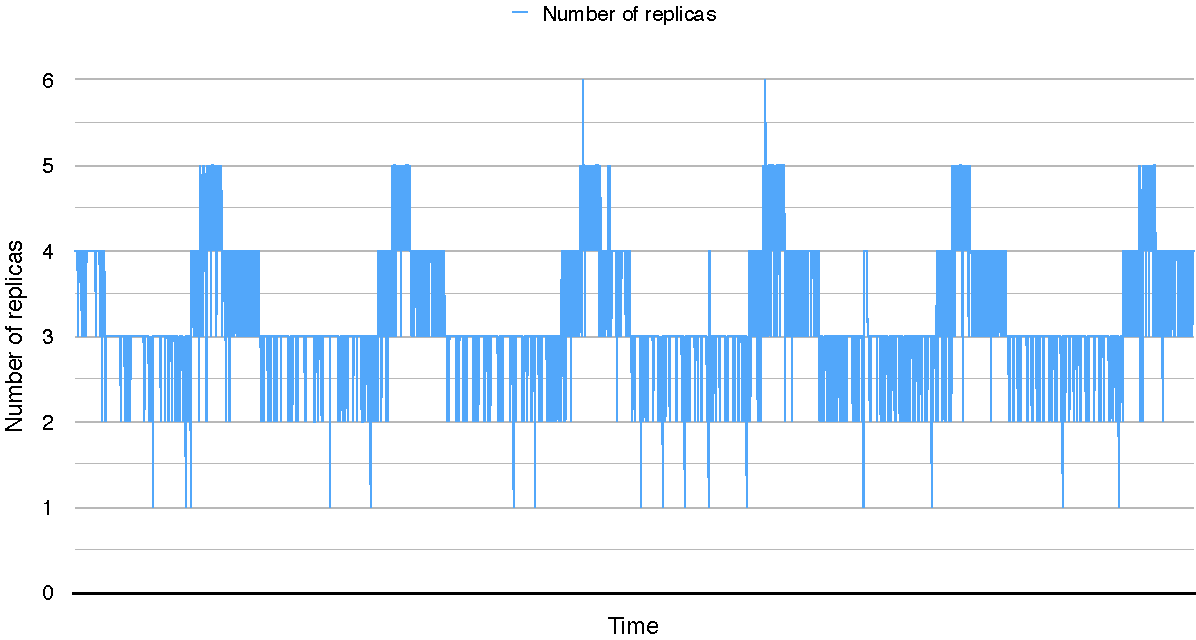
\includegraphics[scale=0.5]{images/results/self_adaptive_replicas.pdf}
\caption[Total number of replicas in~\cref{sec:eval_adaptive_rel_model}]{Result for~\cref{sec:eval_adaptive_rel_model}. Number of replicas over time.} \label{fig:eval_self_adaptive_rel}
\end{figure}

\begin{figure}[!hbt]
\centering
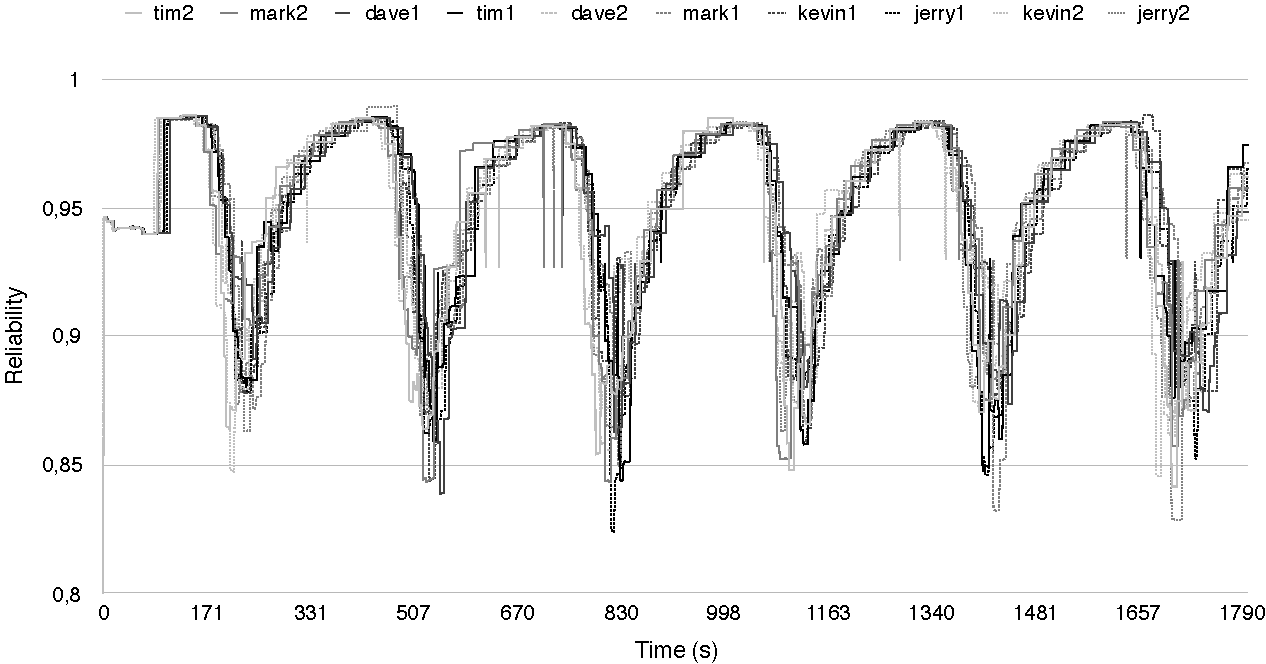
\includegraphics[scale=0.5]{images/results/self_adaptive_node_rels.pdf}
\caption[Nodes reliabilities in~\cref{sec:eval_adaptive_rel_model}]{Result for~\cref{sec:eval_adaptive_rel_model}. The various nodes reliabilities over time.} \label{fig:eval_self_adaptive_node_rels}
\end{figure}

\subsection{Energy efficient for many applications} \label[exp]{sec:eval_energy_efficient}
In this experiment, two runtimes were started on each of the unstable servers. The \emph{MTBF} for the runtimes were the same as for experiment~\cref{sec:eval_opt_nbr_replicas}, and shown in~\cref{table:exp_nodes_means}.

Furthermore, in this experiment five applications were started instead of only one. The applications were identical, described in~\cref{sec:eval_application}, with a required reliability of 0.99999.

Since the replicas are placed on the most reliable nodes, each application will have its replicas on the same nodes, i.e. the most reliable ones. Therefore, theoretically, the total number of nodes having a replica will be no greater than the number of replicas for the application with the most number of replicas. The experiment is therefore considered successful if the number of nodes used at any time were kept to a minimum.

\subsubsection*{Results}
The experiment ran for 5 minutes, and \cref{fig:eval_energy_efficient_total} shows the total number of nodes used over time. \Cref{fig:eval_energy_efficient_mtbf_40}, \cref{fig:eval_energy_efficient_mtbf_15}, and \cref{fig:eval_energy_efficient_mtbf_75} show the number of replicas running at the various nodes. Since the model does not place two replicas of the same task on the same node, the nodes had at most 5 actors, one replica per application, at any time.

The average of the 95th percentile values for the replication time, $t_R$ was during the experiment 763,4 ms. This resulted in that when the system had learned the nodes' \emph{MTBF}, only two replicas per application was needed to reach the required reliability, while three replicas were needed when the \emph{MTBF} was unknown and the default value of 10 seconds was used. As shown in the figure, the number of nodes used varies between two to three for the most time, until after about two minutes, after which only two nodes are needed most of the time. Despite having 10 nodes, at most 4 were actually used to at any time. The experiment was therefore considered successfully.

\begin{figure}[!hbt]
\centering
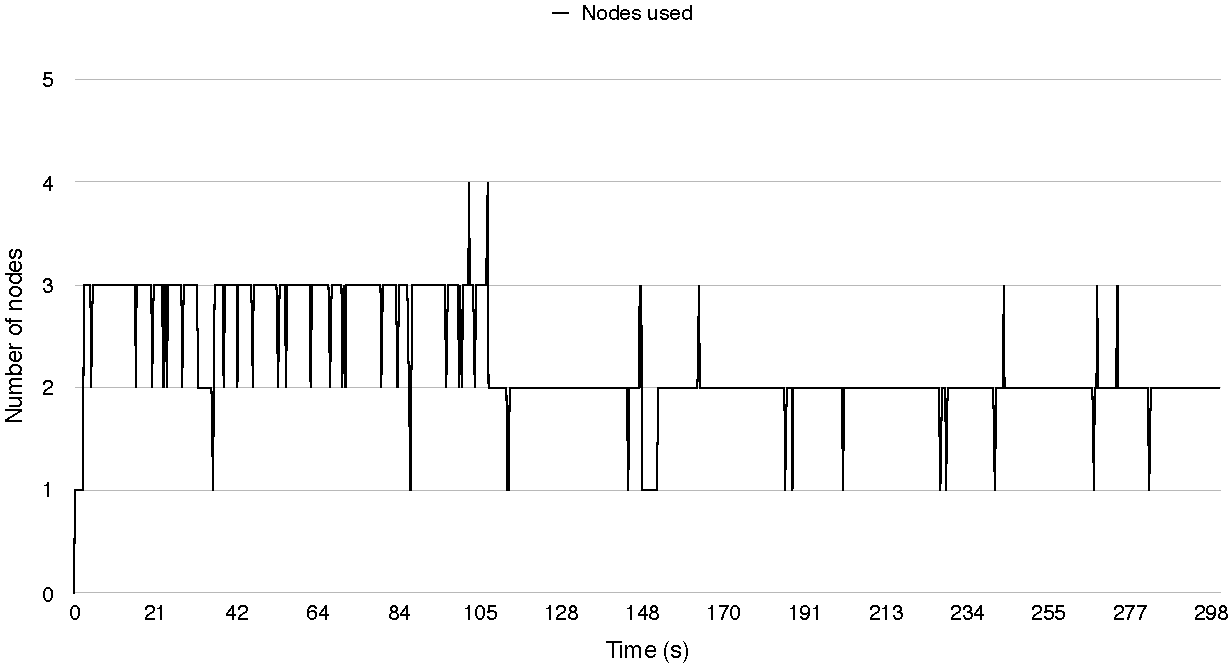
\includegraphics[scale=0.5]{images/results/energy_efficient/total.pdf}
\caption[Total number of nodes used in~\cref{sec:eval_energy_efficient}]{Result for~\cref{sec:eval_energy_efficient}. Number of nodes used.} \label{fig:eval_energy_efficient_total}
\end{figure}

\begin{figure}[!hbt]
\centering
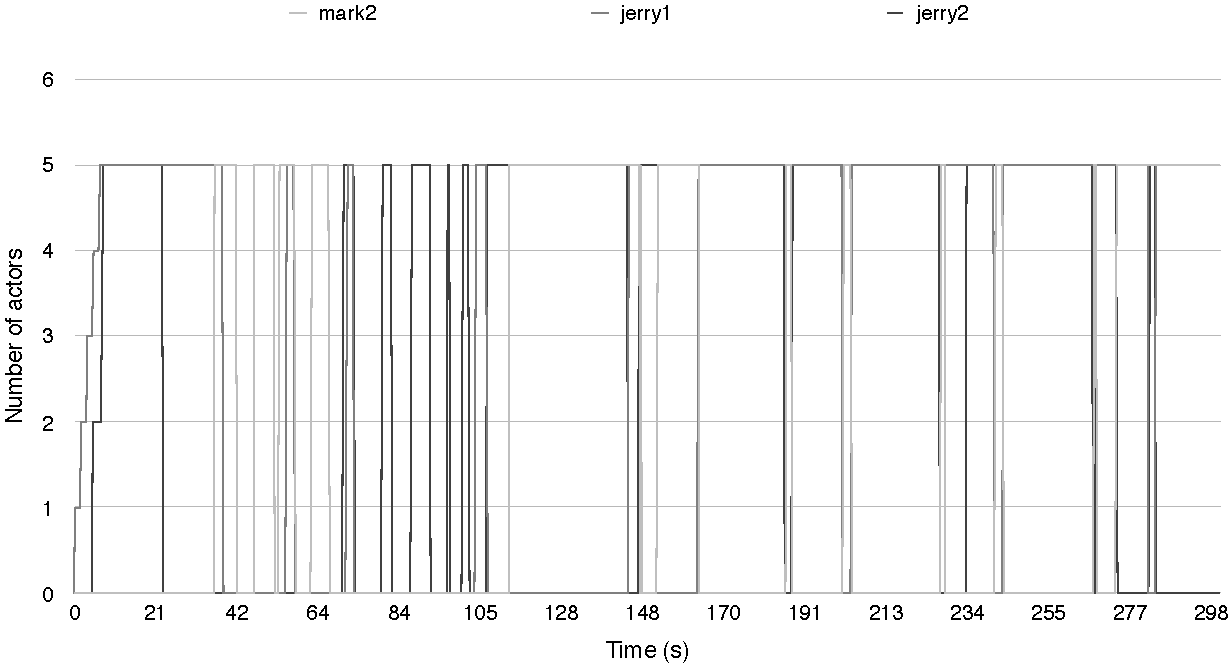
\includegraphics[scale=0.5]{images/results/energy_efficient/MTBF_40.pdf}
\caption[Number of replicas per node in~\cref{sec:eval_energy_efficient} for nodes with \emph{MTBF} = 40 s]{Result for~\cref{sec:eval_energy_efficient}. Number of actors per node, for the three nodes with a \emph{MTBF} of 40 seconds.} \label{fig:eval_energy_efficient_mtbf_40}
\end{figure}

\begin{figure}[!hbt]
\centering
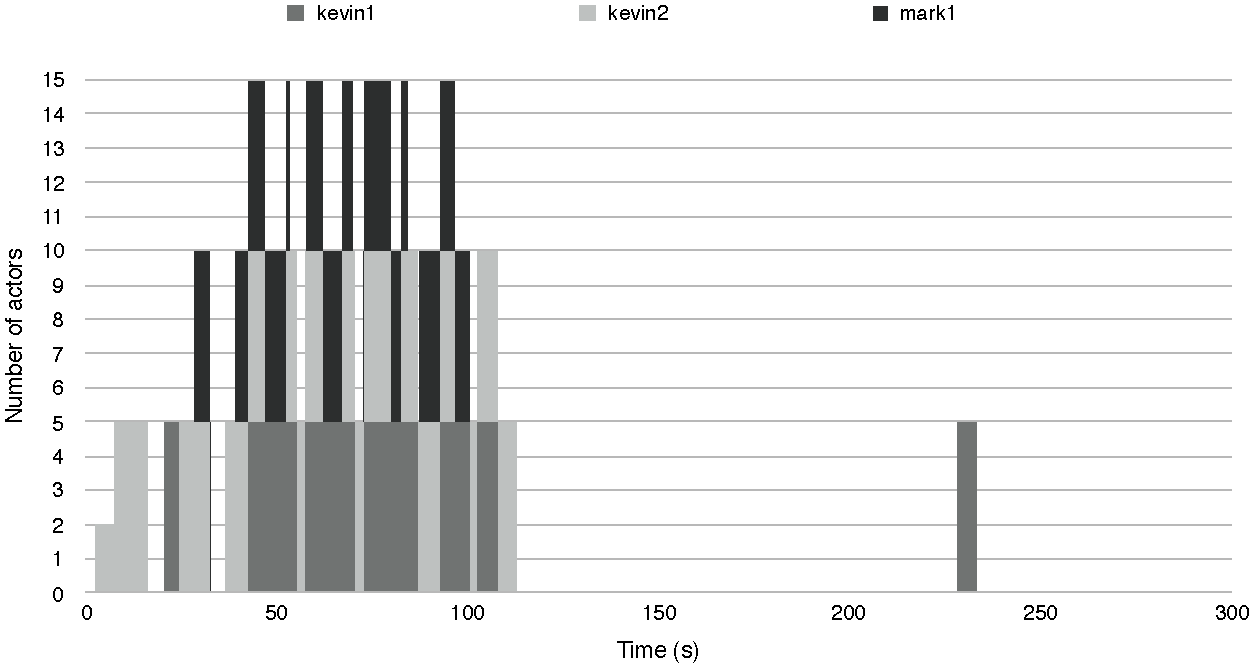
\includegraphics[scale=0.5]{images/results/energy_efficient/MTBF_15.pdf}
\caption[Number of replicas per node in~\cref{sec:eval_energy_efficient} for nodes with \emph{MTBF} = 15 s]{Result for~\cref{sec:eval_energy_efficient}. Number of actors per node, for the three nodes with a \emph{MTBF} of 15 seconds.} \label{fig:eval_energy_efficient_mtbf_15}
\end{figure}

\begin{figure}[!hbt]
\centering
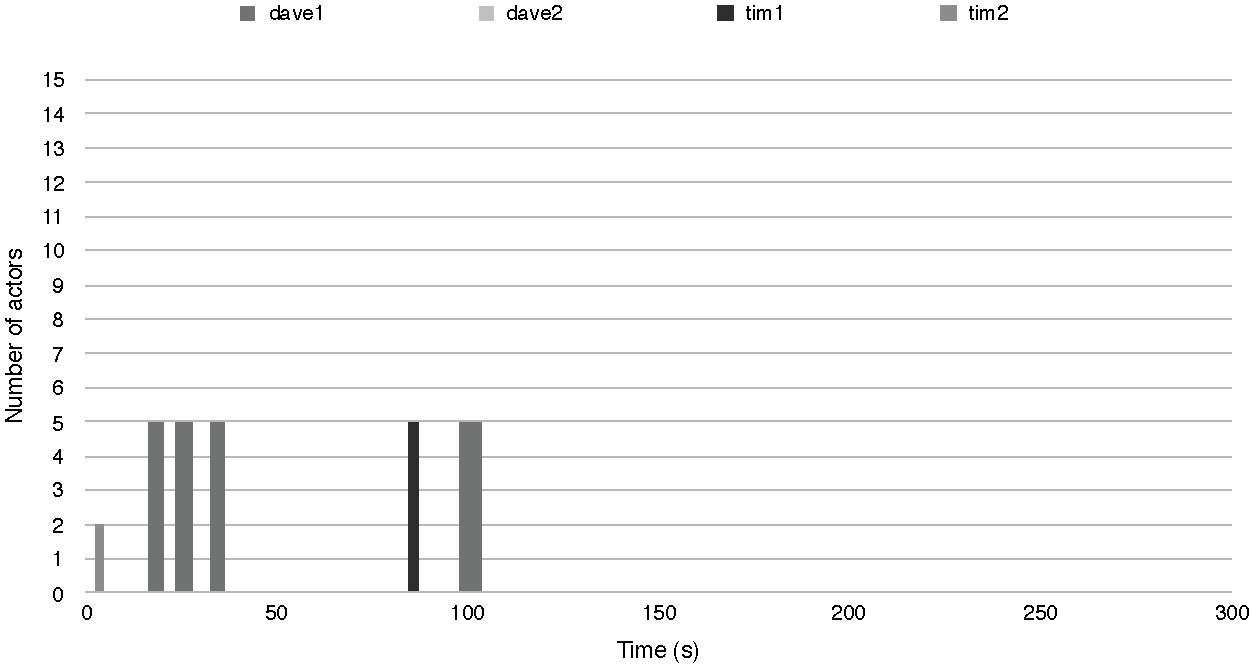
\includegraphics[scale=0.5]{images/results/energy_efficient/MTBF_75.pdf}
\caption[Number of replicas per node in~\cref{sec:eval_energy_efficient} for nodes with \emph{MTBF} = 7.5 s]{Result for~\cref{sec:eval_energy_efficient}. Number of actors per node, for the three nodes with a \emph{MTBF} of 7.5 seconds.} \label{fig:eval_energy_efficient_mtbf_75}
\end{figure}

\subsection{Considering nodes' load} \label[exp]{sec:eval_replaceable_model}
Lastly, to show that the reliability model and selection of nodes to place replicas on are replaceable with more sophisticated algorithms, we conducted an experiment where the system avoids placing replicas on nodes with a CPU usage above 15 percent. 

In this experiment, one runtime was started on each of the unstable servers. Three of the runtimes, \emph{Tim}, \emph{Mark}, and \emph{Jerry}, had a \emph{MTBF} of 10 seconds, and two, \emph{Dave} and \emph{Kevin}, had a \emph{MTBF} of 40 seconds. Furthermore, the load on \emph{Kevin} was increased after a while by starting dummy jobs simply to consume CPU resources, and was later decreased again. The required reliability in this experiment was set to 0.999.

The experiment was considered successful if, despite being one of the more reliable nodes, the system avoided to place replicas on \emph{Kevin}, during the time its load was above the threshold of 15 percent.

\subsubsection*{Results}
The experiment ran for 5 minutes. \Cref{fig:eval_replaceable_model_usages} shows the CPU usage for the various nodes. \Cref{fig:eval_replaceable_model_loaded} and \cref{fig:eval_replaceable_model_unloaded} show the number of replicas for \emph{Kevin} and the other nodes during the experiment.

The average of the 95th percentile values for the replication time, $t_R$ was during the experiment 547,9 ms.

\Cref{fig:eval_replaceable_model_loaded} clearly shows that no replica was placed on \emph{Kevin} during the time its load exceeded the threshold of 15 percent and therefore, this experiment is considered successful. 

This experiment also shows that our model is general and key components such as calculating the reliability of a node as well as sorting the available nodes may be replaced.

\begin{figure}[!hbt]
\centering
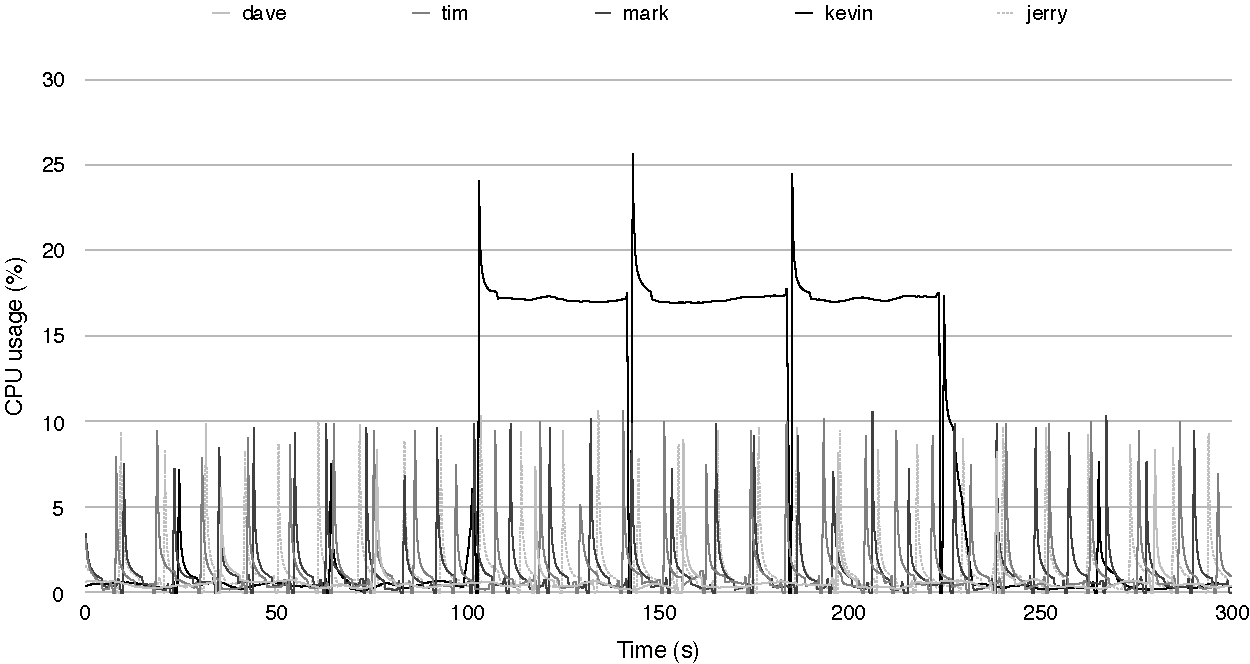
\includegraphics[scale=0.5]{images/results/loads/usages.pdf}
\caption[CPU usage for nodes in~\cref{sec:eval_replaceable_model}]{CPU usages in percent for the nodes used in~\cref{sec:eval_replaceable_model}.} \label{fig:eval_replaceable_model_usages}
\end{figure}

\begin{figure}[!hbt]
\centering
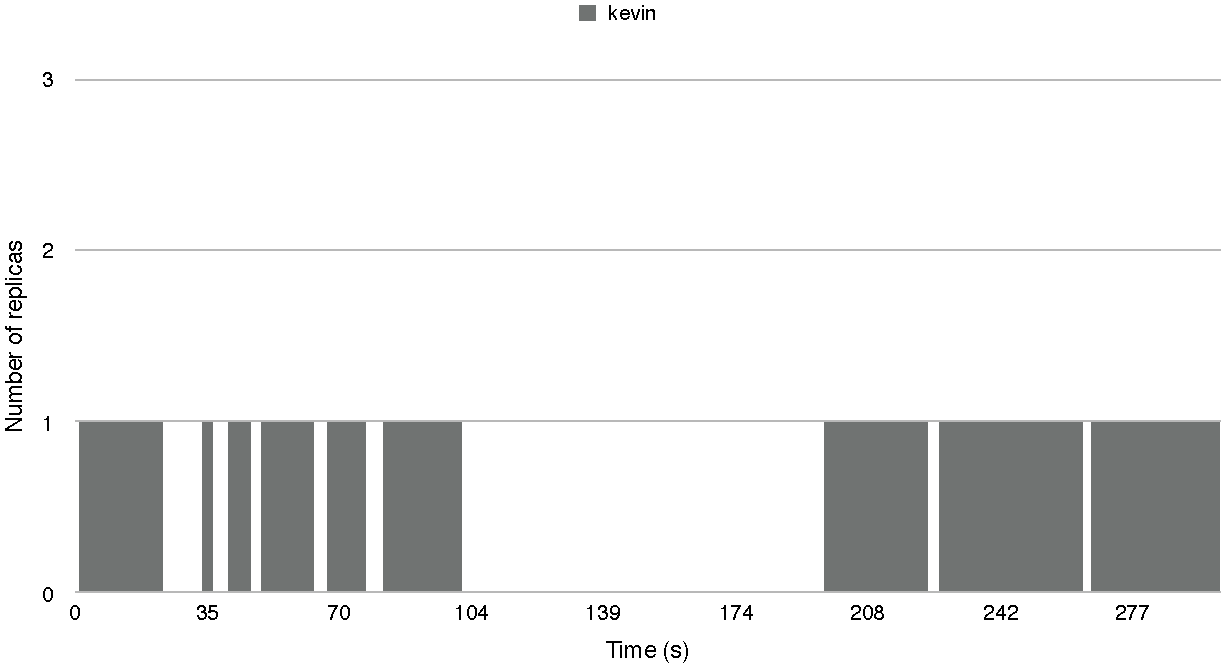
\includegraphics[scale=0.5]{images/results/loads/loaded.pdf}
\caption[Number of replicas on node \emph{Kevin} in~\cref{sec:eval_replaceable_model}]{Result for~\cref{sec:eval_replaceable_model}. The number of replicas over time for node \emph{Kevin}.} \label{fig:eval_replaceable_model_loaded}
\end{figure}

\begin{figure}[!hbt]
\centering
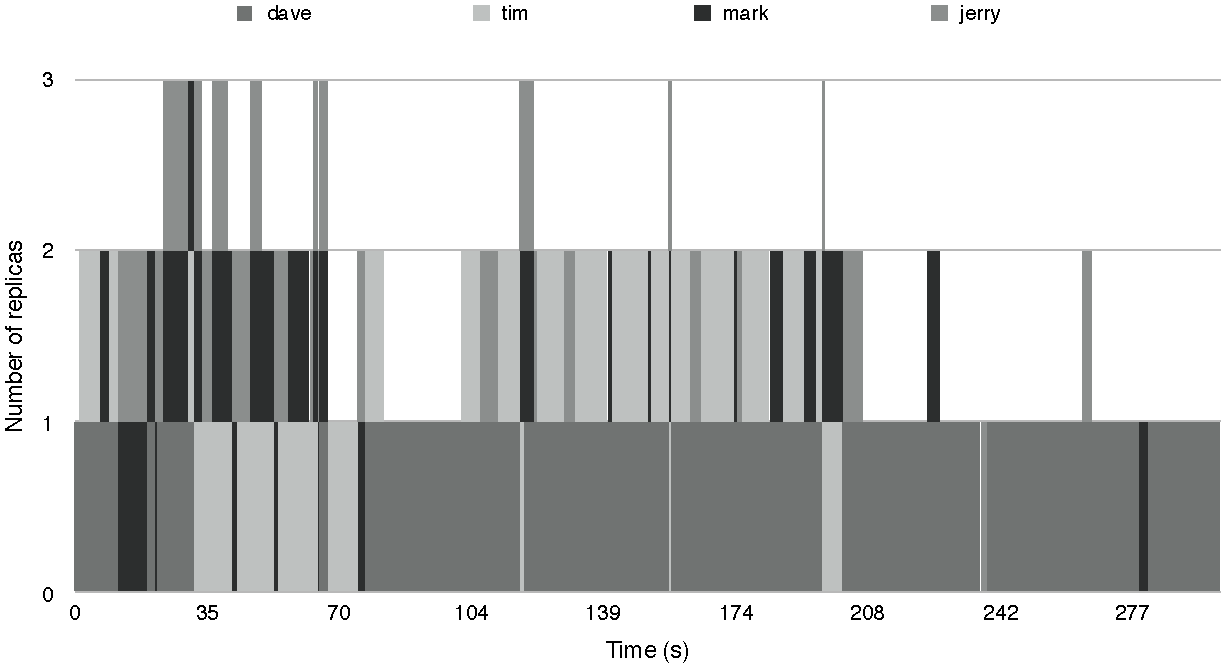
\includegraphics[scale=0.5]{images/results/loads/unloaded.pdf}
\caption[Number of replicas in~\cref{sec:eval_replaceable_model}, all nodes but \emph{Kevin}]{Result for~\cref{sec:eval_replaceable_model}. The number of replicas per node for \emph{Tim}, \emph{Mark}, \emph{Jerry}, and \emph{Dave}.} \label{fig:eval_replaceable_model_unloaded}
\end{figure}

\chapter{Discussion} \label{ch:discussion}
\iffalse
Större drag, vad kan vi få ut av alla experimenten?
Hur mycket kan vi lite på resulaten?
Är det worst-case/best-case?
Kommer det bara bli bättre/snabbare med tiden?
Generalla slutsater
Vi kan ej generalisera våra resultat. typ.
\fi

%TODO
%what if node that deployed an application dies? Then that app want be monitored, solve by choosing one node doing the monitoring.

The reliability model used in this thesis is fairly simple, and has several limitations. Firstly, it requires a node to have failed at least twice before knowing its \emph{MTBF}, otherwise a default value is used. In case the default value is higher than the actual, it results in the calculated reliability of a node, using~\cref{eq:task_reliability_2}, is lower than the actual, before the node has failed twice. Secondly, even though dynamically adapting a node's \emph{MTBF} by using only the three latest failure times, it takes two new failures before the calculated \emph{MTBF} correctly reflects the node's new behavior. Imagine a node failing once every week. After some time, it for some reason starts failing every hour. Then the calculated \emph{MTBF} for that node will be one hour first after it has failed three times with the higher failure rate. Until then, the calculated \emph{MTBF} will be higher, and thereby the calculated reliability will also be higher than the actual. Since periodically monitoring the reliability, some machine learning technique would be beneficial to try predict the reliability of nodes. This would also be beneficial if the system load varies in a periodic way, for instance with higher load during daytime and lower load during night. Since failures are likely to occur when the system load is high some machine learning technique could easily adapt to this behavior and take appropriate preventive actions, like creating new replicas just before daytime.

Moreover, if a node fails frequently in the beginning of its lifetime, and then stabilizes, its \emph{MTBF} will still be based on the registered failure times, resulting in it having a low calculated \emph{MTBF}. Therefore, one could argue that the time since the last registered failure should be considered in the reliability model for a node.

Although our reliability model is fairly simple, \cref{alg:scheduling} is designed to use the reliability model in a plugin fashion, namely by calling~\cref{func:calc_reliability}. This allows for easily replacing the reliability model without changing the algorithm itself. Furthermore, determining on which node to place a new replica also involves an external function call. In our case, the most reliable node is selected, since the available nodes are sorted after reliability, see~\cref{func:sort}. This function could also be replaced without changing the scheduling algorithm. One could for example exclude nodes where the load is above a given threshold, as shown in~\cref{sec:eval_replaceable_model}.

Our model ensures that the reliability is higher than the required as long as we do not experience a node failure. After a node failure and before the system has recovered, by creating new replicas, the reliability is lower than the required. Our model does therefore not guarantee that the average reliability is higher than the required, it depends mainly on the relationship between the \emph{MTBF} and the time it takes to replicate a task, but also on how much above and below the required reliability the momentary reliability is.

Furthermore, to recover from a failure, the failures must be detectable. This is achieved using the heartbeat system described in~\cref{subsec:heartbeats}. If the application consists of several tasks being replicated, as shown in~\cref{fig:extended_app_model}, the heartbeat system will no longer be necessary. Assume we have two tasks $A$ and $B$, with replicas $A_1$, $A_2$ and $B_1$, $B_2$, where $A_1$ and $A_2$ both send their results to $B_1$ and $B_2$. Such a situation would allow to use a fault model which in addition to node failures also consider task and link failures. A task failure is detected if both replicas of $B$ stop receiving results from $A_1$ or $A_2$. Furthermore, link failures are detected if for instance $B_1$ receives result from both $A_1$ and $A_2$ while $B_2$ only receives results from $A_1$. The link between $A_2$ and $B_2$ is then likely to have failed. This is however based on the assumption that the task $A$ periodically sends results to $B$.

Moreover, the assumption of a fully reliable network with redundant paths is unlikely to reflect the real characteristics of distributed systems. In case of a link failure in a real setting, some nodes may not receive heartbeats from a node, while others will. The nodes not receiving the heartbeat will then falsely assume the node has died. Such a situation may result in new replicas being created, perhaps more than necessary, and thereby putting an unnecessarily high demand on the system in terms of resource usage. Although, since the optimization algorithm in run periodically, the unnecessary replicas will eventually be removed.

We further assume tasks always will produce the correct result. Since the receiving task will receive a result of each replica, some consensus algorithm such as \emph{majority voting} or \emph{k-modular redundancy} could be implemented at the receiver side. Thereby, one could adapt the broader Byzantine fault model instead of the fail-stop model. This also allows for changing the reliability definition from not the probability of producing a result, but also to produce the correct result.

With the primary objective being to ensure a certain level of reliability, and doing so using active replication, we require much more resources, which puts an extra burden on the system. The extra load on the system may affect tasks' execution time, thus decreasing task performance. However, using active replication instead of checkpointing or rollback recovery, the extra time needed in case of failure is avoided, and in such cases the execution time may instead be improved by using replication. Furthermore, since we minimize the number of replicas used for each application, by placing replicas on the most reliable nodes, we consequently use the minimum number of nodes overall, as shown in~\cref{sec:eval_energy_efficient}. Our model is therefore energy efficient, although the nodes not used are not shut down, nor put in idle mode.

In our experiments we replicated only one of the tasks in the used application. When handling a lost node, \cref{alg:scheduling} must be run for every task which had a replica on the lost node. In a more realistic setting, there will likely be several different task replicas on the lost node. One must therefore decide in which order the tasks should be handled, and create new replicas for if needed. One possible solution is to prioritize all tasks, and start replicating the task with highest priority. However, the time $t$ used in the reliability model is defined as the time it takes from that a failure occur until a new replica is operational. Therefore, when handling a lost node and start measuring the time, all tasks on the lost node will have the same start time. This will result in that the task with the lowest priority will have the largest time $t$, since it will be handled last. Since this affects the reliability, the task with the lowest priority will thereby require the most number of replicas. Consequently, the task with lowest priority requiring the most resources. However, in~\cref{sec:eval_energy_efficient} we had five applications, and consequently five tasks being replicated from the same node in case of node failures. This explains why the average replication time, mentioned in~\cref{sec:eval_energy_efficient} is higher than in most of the other experiments. In the experiment we simply replicated the tasks in random order.

As mentioned, the reliability is dependent on the replication time, which depends on the state of the task to replicate. The Calvin framework is only designed for light-weight IoT applications, thus not for applications where the actor state is several megabytes, and not optimized for replicating actors of such sizes. Despite this, our experiments show that it takes less than 40 minutes to replicate an actor with a state of 1 gigabyte between two servers in the same cluster. Assuming a \emph{MTBF} of one year (31536000 s), and a time $t$ of 1 hour (3600 s) for detecting and replicating, having only two replicas gives using \cref{eq:task_reliability_2} a reliability of

\begin{equation*}
\begin{split}
R_{T}(3600) = 1 - \prod\limits_{k=1}^2 F_{k}(3600)\\
= 1 - \prod\limits_{k=1}^2 (1 - R(3600))\\
= 1 - (1 - e^{3600/31536000})^2\\
= 0.9999999863
\end{split}
\end{equation*}

This means despite having a large time $t$, a high reliability can be achieved by only having two replicas. 



\chapter{Future Work} \label{ch:future_work}
To the best of our knowledge, our model is the first of its kind, due to its fully dynamic behavior. Furthermore, the implementation provides a means to carry out experiments. Thereby, there are many possibilities for future work. 

Our model could be extended by considering more types of failures such as link failures, task failures, but also but tasks not producing the correct result. In the latter case, some consensus algorithm could be implemented in order to hamper the risk of using incorrect results. Link failures could for instance be detected if the node responsible for handling the node failure awaits request from several nodes before running~\cref{alg:scheduling}. If a node receives only a single \emph{lost node} message, it is likely that the node is still alive but the link between the node and the sender of the \emph{lost node} message has failed.
 
The process of selecting where to place new replicas could be extended to consider whether or not the selected node has capacity for the new replica. The application author could, using some metric, define the resources needed for a task replica, and the system administrator assign each node a metric of their capacities. These metrics could then be used to determine whether or not the available nodes have the required capacity for a replica.

Furthermore, as mentioned in~\cref{ch:discussion}, our model is energy efficient as it will use the minimum number of nodes. However, this is based on the assumption that nodes always have enough capacity for the replicas placed on them. If the available capacity of nodes and the required capacity needed by the tasks are taken into account, the task placement decision is turned into a bin-packing problem for optimizing the number of nodes needed. By further extending the system with functionality for dynamically shutting down/starting nodes, unused nodes could be shut down to save energy and money.

Besides from considering additional types of failures and the capacity of nodes, our model would benefit greatly from applying some machine learning technique. By predicting when the nodes are about to get overloaded, or the reliability of nodes are about to decrease, one could take preventative measures, e.g. move replicas to other nodes.

Our model is yet to be evaluated on highly unreliable system during extreme load. In such a case, due to the unreliability of the system, the number of replicas needed to ensure the required reliability level will increase. This will further increase the system load, thereby decreasing the reliability of the system even further, which may turn into a vicious circle.

Furthermore, since the replication time as mentioned depends on the number of other tasks being handled before, the reliability is affected by the number of other tasks running on the same node. This should either be considered in the reliability model, or the handling of failures must be changed. Instead of selecting a single node responsible for handling the failures, one node could be selected for each replica lost. The time $t$ would thereby no longer be dependent on how many other tasks were running on the lost node.

If a single node is used to handle all lost replicas, one must consider in which order they are handled. One way would be to replicate the actors with the biggest states first in order to achieve a uniform distribution of the replication times, or to handle the highest priority tasks first as described in~\cref{ch:discussion}. We leave the investigation of which algorithm is the optimal to future work. 

Furthermore, our model does not guarantee that the average of the actual reliability is above the required, it only aims at keeping the momentary reliability higher than the required. This allows for the user specifying various reliability requirements. One such requirement could be that the time the system is in a vulnerable state should not exceed some threshold. Keeping the average reliability above a required level could be achieved by calculating the current average based on the quote between \emph{MTBF} and $t_r$, replication time. In the simplest case, when all nodes have the same \emph{MTBF} this could be achieved by using \cref{eq:avg_rel_same_MTBF}.

\begin{equation} \label{eq:avg_rel_same_MTBF}
	\frac{(MTBF/n - t_{R})}{(MTBF/n)} \cdot R^n + \frac{t_{R}}{(MTBF/n)} \cdot R^{n-1}
\end{equation}

Our model is also to be tested using geographically distributed clusters. If such a case, one must take into account that the replication time will be higher when replicating to a node in another cluster than within the same cluster. Furthermore, whether or not the heartbeat system and handling of lost nodes should be done globally or only locally within a cluster is yet to be investigated.

Finally, assuming statistically independent failures, the reliability of a node depends only on the time $t$, and the node's \emph{MTBF}. However, since failures are likely to not be statistically independent, they should be taken into account in the reliability model. For example, if the switch of a rack fails, all nodes in that rack are unavailable. Therefore, the reliability of when having two replicas placed on two nodes in the same rack, is likely less than the reliability of two replicas placed on nodes in different racks.


\chapter{Conclusions} \label{ch:conclusions}
The goal of this thesis was first to devise a method for dynamically ensuring a predefined level of reliability for distributed applications or services. This was accomplished by first designing a somewhat simplistic reliability model, and secondly a framework which automatically detects node failures and ensures the predefined reliability is met. 

The predefined reliability is ensured by replication of tasks, and based on the available resources the framework creates enough number of replicas. In order to optimize the number of replicas over time the system is periodically monitored in order to dynamically adapt to resources' changing behavior.

Furthermore, the goal was also to provide a platform to be used to further experiments. This was accomplished by implementing our model using Calvin. Both the reliability model used and the task placement function are replaceable, which gives rise to various experimental opportunities. One could for instance include resources' load and capacity in the task place function or apply machine learning in the reliability function, but this is left as future work.


\iffalse
GOAL - copied:

The goal of this thesis is to devise a method for dynamically ensuring a predefined level of reliability for distributed applications or services. Reliability will be achieved by replicating tasks. 

First, a reliability model will be designed, describing the reliability of the available resources, and for applications using these resources.

Secondly, a framework will be designed which will automatically detect node failures and based on the reliability of the available resources creates enough replicas to reach the required reliability level.

Lastly, the system and its running applications will be periodically monitored in order to adapt the resources' reliability and the number of replicas needed as the properties of the system varies over time.

The model will be implemented and tested using the IoT application framework \emph{Calvin}.
\fi

\begin{thebibliography}{50}

%TODO
% Innan final
% http://libguides.lub.lu.se/referencemanagement_lth
% IEEE reference style

\bibitem{taskAllocation}
	S. M. Shatz, J. Wang and M. Goto,
	"Task Allocation for Maximizing Reliability of Distributed Computer Systems",
	\emph{IEEE Transactions on Computers}, vol. 41, no. 9, pp. 1156-1168, Sep. 1992.
	
\bibitem{surveyReliabilityDistr}
	W. Ahmed and Y. W. Wu,
	"A survey on reliability in distributed systems",
	\emph{Journal of Computer and System Sciences}, vol. 78, no. 8,	pp. 1243–1255, Dec. 2013.
	
\bibitem{surveyRelPrediction}
	A. Immonen and E. Niemelä,
	"Survey of reliability and availability prediction methods from the viewpoint of software architecture",
	\emph{Software \& Systems Modeling}, vol. 7, no. 1, pp. 49-65, Feb. 2008.

\bibitem{relDistApplications}
	C. A. Tănasie, S. Vîntutis and A. Grigorivici,
	"Reliability in Distributed Software Applications",
	\emph{Informatica Economică}, vol. 15, no. 4, pp. 167-177, 2011,

\bibitem{relGridSystems}
	C. Dabrowski,
	"Reliability in grid computing systems",
	\emph{Concurrency Computation: Practice Experience  - A Special Issue from the Open Grid Forum}, vol. 21, no. 8, pp. 927-959, June 2009.

\bibitem{compStudyLoadAndCloud}
	M. Katyal and A. Mishra,
	"A Comparative Study of Load Balancing Algorithms in Cloud Computing Environment",
	\emph{International Journal of Distributed and Cloud Computing}, vol. 1, no. 2, pp. 5-14, Dec. 2013.
	
\bibitem{relAndPerfGridServices}
	Y. Dai and G. Levitin,
	"Reliability and Performance of Tree-Structured Grid Services",
	\emph{IEEE Transactions on Reliability}, vol. 55, no. 2, pp. 337-349, June 2006.

\bibitem{surveyFaultParallel}
	M. Treaster,
	"A Survey of Fault-Tolerance and Fault-Recovery Techniques in Parallel Systems",
	\emph{Cornell University Library}, Jan. 2005.

\bibitem{faultTolerantFundamentals}
	F. C. Gärtner,
	"Fundamentals of Fault-Tolerant Distributed Computing in Asynchronous Environments",
	\emph{ACM Computing Surveys}, vol. 31, no. 1, pp. 1-26, Mar. 1999.

\bibitem{perfAnalysisLoadCloud}
	K. Garala, N. Goswami and P. Maheta,
	"A Performance Analysis of Load Balancing Algorithms in Cloud Environment",
	\emph{2015 International Conference on Computer Communication and Informatics (ICCCI)}, pp.1-6, Jan. 2015.
	
\bibitem{taskSchedulingReplication}
	S. Wang, K. Li, J. Mei, K. Li and Y. Wang,
	"A Task Scheduling Algorithm Based on Replication for Maximizing Reliability on Heterogeneous Computing Systems",
	\emph{28th IEEE International Parallel \& Distributed Processing Symposium Workshops (IPDPSW)}, pp. 1562-1571, May 2014.

\bibitem{dynAdaptRepl}
	Z. Guessoum, J. Briot, O. Marin, A. Hamel and P. Sens,
	"Dynamic and Adaptive Replication for Large-Scale Reliable Multi-agent Systems",
	\emph{Lecture Notes in Computer Science}, vol. 2603, pp 182-198, Apr. 2003.

\bibitem{algoMaxRelEndToEndConstraint}
	F. Cao and M. Zhu,
	"Distributed workflow mapping algorithm for maximized reliability under end-to-end delay constraint",
	\emph{The Journal of Supercomputing}, vol. 66, no. 3, pp. 1462-1488, Dec. 2013.

\bibitem{algoMinExTime}
	A. Dogan and F. Özüner,
	"Matching and Scheduling Algorithms for Minimising Execution Time and Failure Probability of Applications in Heterogeneous Computing",
	\emph{IEEE Transactions on Parallel and Distributed Systems}, vol. 13, no.3, pp. 308-323, Mar. 2002.

\bibitem{relModelDistSimSystem}
	H. Wan, H. Huang, J. Yang and Y. Chen,
	"Reliability model of distributed simulation system",
	\emph{2011 International Conference on Quality, Reliability, Risk, Maintenance, and Safety Engineering (ICQR2MSE)}, pp. 99-104,	June 2011.

\bibitem{relModelAnalysis}
	C. S. Raghavendra and S. V. Makam,
	"Reliability Modeling and Analysis of Computer Networks",
	\emph{IEEE Transactions on Reliability}, vol. 35, no. 2, pp. 156-160, June 1986.

\bibitem{cloudServiceRel}
	Y. Dai, B. Yang, J. Dongarra and G. Zhang,
	"Cloud Service Reliability: Modeling and Analysis",
	\emph{15th IEEE Pacific Rim International Symposium on Dependable Computing}, Nov. 2009. %TODO pages?

\bibitem{optTaskAllocationForMaxRel}
	H. Faragardi, R. Shojaee, M. Keshtkar and H. Tabani,
	"Optimal task allocation for maximizing reliability in distributed real-time systems",
	\emph{12th International Conference on Computer and Information Science (ICIS), 2013 IEEE/ACIS}, pp. 513-519, June 2013.

\bibitem{perfImplPerCheckPoint}
	A. J. Oliner, R. K. Sahoo, J. E. Moreira and M. Gupta,
	"Performance Implications of Periodic Checkpointing on Large-scale Cluster Systems",
	\emph{19th IEEE International Parallel and Distributed Processing Symposium}, Apr. 2005. %TODO pages?

\bibitem{studyOfFailures}
	B. Schroeder and G. Gibson,
	"A large-scale study of failures in high-performance computing systems",
	\emph{IEEE Transactions on Dependable and Secure Computing}, vol. 7, no. 4, pp.337-350, Nov. 2010.

\bibitem{implicationsOfFailures}
	Y. Zhang, M. S. Squillante, A. Sivasubramaniam and R. K. Sahoo,
	"Performance Implications of Failures in Large-Scale Cluster Scheduling",
	\emph{Lecture Notes in Computer Science }, vol. 3277, pp. 233-252, 2005. %TODO no.?

\bibitem{discContRelModel}
	L. Fiondella, and L. Xing,
	"Discrete and continuous reliability models for systems with identically distributed correlated components",
	\emph{Reliability Engineering \& System Safety}, vol. 133, pp. 1-10, Jan. 2015. %TODO no.?

\bibitem{effTaskReplMobGrid}
	A. Litke, D. Skoutas, K. Tserpes and T. Varvarigou,
	"Efficient task replication and management for adaptive fault tolerance in Mobile Grid environments",
	\emph{Future Generation Computer Systems}, vol. 23, no. 2, pp. 163-178, Feb. 2007.

\bibitem{realTimeSchedAlgo}
	Y. Ling and Y. Ouyang,
	"Real-time fault-tolerant scheduling algorithm for distributed computing systems",
	\emph{Journal of Digital Information Management}, vol. 10, no. 5, pp. 289-294, Oct. 2012.

\bibitem{optCheckpointInterval}
	J.T. Daly,
	"A higher order estimate of the optimum checkpoint interval for restart dumps",
	\emph{Future Generation Computer Systems}, vol. 22, no. 3, pp. 303-312, Feb. 2006.

\bibitem{factorsAffectingRel}
	X. Zhang and H. Pham,
	"An analysis of factors affecting software reliability",
	\emph{The Journal of Systems and Software}, vol. 50, no. 1, pp. 43-56, Jan. 2000.

\bibitem{algoOptTimeMaxRel}
	P. Saxena and K. Govil,
	"An Algorithm for Optimized Time, Cost, and Reliability in a Distributed Computing System",
	\emph{International Journal of Advanced Networking and Applications}, vol. 4, no. 5, pp. 1710-1718, Apr. 2013.

\bibitem{imprRelAdaptRL}
	M. Hussin, N. A. W. A Hamid and K. A. Kasmiran,
	"Improving reliability in resource management through adaptive reinforcement learning for distributed systems",
	\emph{Journal of Parallel and Distributed Computing}, vol. 75, pp. 93-100, Jan. 2015

\bibitem{selfAdaptRel}
	Y. Brun, J. Bang, G. Edwards and N. Medvidovic,
	"Self-Adapting Reliability in Distributed Software Systems",
	\emph{IEEE Transactions on Software Engineering}, vol. 41, no. 8, pp. 764-780, Aug. 2015.

\bibitem{schedReplicas}
	P. Chevochot and I. Puaut,
	"Scheduling Fault-Tolerant Distributed Hard Real-Time Tasks Independently of the Replication Strategies",
	\emph{Sixth International Conference on Real-Time Computing Systems and Applications, 1999. RTCSA '99}, pp. 356-363, Dec. 1999.

\bibitem{calvin}
	P. Persson and O. Angelsmark,
	"Calvin - Merging Cloud and IoT",
	\emph{Procedia Computer Science}, vol. 52, pp. 210–217, 2015

\bibitem{taskAllocationSwarm}
	P. Yin, S. Yu, P. Wang and Y. Wang,
	"Task allocation for maximizing reliability of a distributed system using hybrid particle swarm optimization",
	\emph{The Journal of Systems and Software}, vol. 80, no. 5, pp. 724-735, May 2007.

\bibitem{optResourceAllMaxPerformance}
	Y. Dai and G. Levitin,
	"Optimal Resource Allocation for Maximizing Performance and Reliability in Tree-Structured Grid Services",
	\emph{IEEE Transactions on Reliability}, vol. 56, no. 3, pp. 444-453, Sep. 2007.

\bibitem{matchSchedAlgoMinFailure}
	A. Dogan and F. Özgüner,
	"Matching and Scheduling Algorithms for Minimizing Execution Time and Failure Probability of Applications in Heterogeneous Computing",
	\emph{IEEE Transactions on Parallel and Distributed Systems}, vol. 13, no. 3, pp. 308-323, Mar. 2002.

\bibitem{safetyRelTaskAllocation} 
	S. Srinivasan and N. K. Jha,
	"Safety and Reliability Driven Task Allocation in Distributed Systems",
	\emph{IEEE Transactions on Parallel and Distributed Systems}, vol. 10, no. 3, pp. 238-251, Mar. 1999.

\bibitem{improvedTaskAllMaxRel}
	S. Kartik, C. Siva Ram Murthy,
	"Improved Task-Allocation Algorithms to Maximize Reliability of Redundant Distributed Computing Systems",
	\emph{IEEE Transactions on Reliability}, vol. 44, no. 4, pp. 575-586, Dec. 1995.

\bibitem{designFaultTolerantSched}
	M. Amoon,
	"Design of a Fault-Tolerant Scheduling System for Grid Computing",
	\emph{2011 Second International Conference on Networking and Distributed Computing}, pp. 104-108, Sept. 2011.

\bibitem{evalReplicationSched}
	M. Chtepen B. Dhoedt, F. Turck, P. Demeester, F. Claeys and P. Vanrolleghem, 
	"Evaluation of replication and rescheduling heuristics for grid systems with varying resource availability",
	\emph{Proceedings of the 18th IASTED International Conference on Parallel and Distributed Computing and Systems}, pp.622-627, Nov. 2006.

\bibitem{faultTolerantSchedPolicy}
	J. H. Abawajy,
	"Fault-Tolerant Scheduling Policy for Grid Computing Systems",
	\emph{Proceedings of the 18th International Parallel and Distributed Processing Symposium}, Apr. 2004.

\bibitem{adaptiveCheckPointAndRep}
	M. Chtepen, F. Claeys, B. Dhoedt, F. Turck, P. Demeester and P. A. Vanrolleghem,
	"Adaptive Task Checkpointing and Replication: Toward Efficient Fault-Tolerant Grids",
	\emph{IEEE Transactions on Parallel and Distributed Systems}, vol. 20, no. 2, Feb. 2009

\bibitem{perfRelNonMarkovian}
	J. E. Pezoa and M. M. Hayat,
	"Performance and Reliability of Non-Markovian Heterogeneous Distributed Computing Systems",
	\emph{IEEE Transactions on Parallel and Distributed Systems}, vol. 23, no. 7, pp. 1288-1301, July 2012.

\bibitem{hierarchicalRelModeling}
	Y. Dai, Y. Pan and X. Zou,
	"A Hierarchical Modeling and Analysis for Grid Service Reliability",
	\emph{IEEE Transactions on Computers}, vol. 56, no. 5, pp. 681-691, May 2007.

\bibitem{relAnalysisFRA}
	D. Chen and T. Huang,
	"Reliability analysis of distributed systems based on a fast reliability algorithm",
	\emph{IEEE Transactions on parallel and distributed systems}, vol. 3, no. 2, pp. 139-154, Mar. 1992.

\bibitem{relGridServicePredConstraint}
	Gregory Levitin, Yuan-Shun Dai and H. Ben-Haim,
	"Reliability and Performance of Star Topology Grid Service with Precedence Constraints on Subtask Execution",
	\emph{IEEE Transactions on Reliability}, vol. 55, no. 3, pp. 507-515, Sept. 2006.

\bibitem{relModelWebServices}
	W. T. Tsai, D. Zhang, Y. Chen, H. Huang, R. Paul and N. Liao,
	"A Software Reliability Model for Web Services",
	\emph{Proceedings of the IASTED Conference on Software Engineering and Applications}, Nov. 2004. %TODO pp?

\bibitem{studyServiceRel}
	Y.S. Dai, M. Xie, K.L. Poh and G.Q. Liu,
	"A study of service reliability and availability for distributed systems",
	\emph{Reliability Engineering and System Safety}, vol. 79, no. 1, pp. 103-112, Jan. 2003.

\bibitem{efficientRelAnalysisAlgo}
	M. Lin, M. Chang and D. Chen,
	"Efficient algorithms for reliability analysis of distributed computing systems",
	\emph{Information Sciences}, vol. 117, no. 1-2, pp. 89-106, July 1999.

\bibitem{evalOfGridRel}
	E. Huedo, R. S. Montero and I. M. Llorente,
	"Evaluating the reliability of computational grids from the end user’s point of view",
	\emph{Journal of Systems Architecture}, vol. 52, no. 12, pp. 727-736, Dec. 2006.

\bibitem{generalAlgoRelEval}
	A. Kumar and D. P. Agrawal,
	"A Generalized Algorithm for Evaluating Distributed-Program Reliability",
	\emph{IEEE Transactions on Reliability}, vol. 42, no. 3, pp. 416-426, Sept. 1993.

\bibitem{realTimeRelAnalysis}
	D. Chen, M. Sheng and M. Homg,
	"Real-Time Distributed Program Reliability Analysis",
	\emph{Proceedings of the Fifth IEEE Symposium on Parallel and Distributed Processing}, pp. 771-778 Dec. 1993.

\bibitem{faultToleranceGrid}
	T. Altameem,
	"Fault Tolerance Techniques in Grid Computing Systems",
	\emph{International Journal of Computer Science and Information Technologies}, vol. 4, no. 6, pp. 858-862, Dec. 2014.

\bibitem{faultToleranceChallenges}
	A. Bala and I. Chana,
	"Fault Tolerance Challenges, Techniques and Implementation in Cloud Computing",
	\emph{International Journal of Computer Science Issues}, vol. 9, no. 1, pp. 288-293, Jan. 2012.

\bibitem{improvingPerformanceReplication}
	Y. Li and, M. Mascagni,
	"Improving Performance via Computational Replication on a Large-Scale Computational Grid",
	\emph{3rd IEEE/ACM International Symposium on Cluster Computing and the Grid}, pp. 442-448, May 2003.

\bibitem{adaptiveMASReplication}
	D. Sylvian, Z. Guessoum and M. Ziane,
	"Adaptive Replication in Fault-Tolerant Multi-Agent Systems",
	\emph{IEEE/WIC/ACM International Conferences on Web Intelligence and Intelligent Agent Technology}, vol. 2, pp. 304-307, Aug. 2011.

\bibitem{replicatingAgents}
	A. Fedoruk and R. Deters,
	"Improving Fault-Tolerance by Replicating Agents",
	\emph{Proceedings of the first international joint conference on Autonomous agents and multiagent systems: part 2}, pp. 737-744, Jan. 2002.

\bibitem{adaptiveAgentReplication}
	Z. Guessoum, J. Briot, N. Faci and O. Marin,
	"Towards Reliable Multi-Agent Systems: An Adaptive Replication Mechanism",
	\emph{ Multiagent and Grid Systems}, vol. 6, no. 1, pp. 1-24, Mar. 2010.

\bibitem{replicationManagement}
	R. Yadav and A. S. Sidhu,
	"Fault Tolerant Algorithm for Replication Management in Distributed Cloud System",
	\emph{2015 IEEE 3rd International Conference on MOOCs, Innovation and Technology in Education (MITE)}, pp. 78-83, Oct. 2015.

\bibitem{experimentalFailureAssessment}
	J. S. Plank and W. R. Elwasif,
	"Experimental Assessment of Workstation Failures and Their Impact on Checkpointing Systems",
	\emph{Digest of Papers. Twenty-Eighth Annual International Symposium on Fault-Tolerant Computing, 1998}, pp. 48-57, June 1998.

\bibitem{schedulingSurvey}
	R. Nallakumar, N. Sengottaiyan and K. S. Sruthi Priya,
	"A Survey on Scheduling and the Attributes of Task Scheduling in the Cloud",
	\emph{International Journal of Advanced Research in Computer and Communication Engineering}, vol. 3, no. 10, pp. 8167-8171, Oct. 2014.

\bibitem{optSchedCloud}
	A. Jangra and T. Saini,
	"Scheduling Optimization in Cloud Computing",
	\emph{International Journal of Advanced Research in Computer Science and Software Engineering}, vol. 3, no. 4, pp. 62-65, Apr. 2013.

\bibitem{vm_vs_container}
	D. Strauss,
	"Containers—Not Virtual Machines—Are the Future Cloud", 
	June 2013. [Online]. \\
	Available:
	 http://www.linuxjournal.com/content/containers\%E2\%80\%94not-virtual-machines\%E2\%80\%94are-future-cloud.
	[Accessed: 25 May 2016].
	
\bibitem{probabilistic_recovery}
	K. R. Joshi, M. A. Hiltunen, W. H. Sanders and R. D. Schlichting,
	"Probabilistic Model-Driven Recovery in Distributed Systems",
	\emph{IEEE Transactions on Dependable and Secure Computing}, vol. 8, no. 6, pp. 913-928, Nov./Dec. 2011.
	
\bibitem{kademlia}
	P. Maymounkov and D. Mazières,
	"Kademlia: A Peer-to-peer Information System Based on the XOR Metric",
	\emph{Lecture Notes in Computer Science}, vol. 2429, pp. 53-65, Oct. 2002.

\bibitem{IEEEfaultTolerantSys} 
	U. Malladi,
	"Notice of Violation of IEEE Publication Principles Design, analysis and performance evaluation of a new algorithm for developing a fault tolerant distributed system",
	\emph{12th International Conference on Parallel and Distributed Systems}, vol. 1, July 2006. %TODO pp?

\bibitem{faultTolerantDeadlock}
	P. Li and B. McMillin,
	"Fault-tolerant distributed deadlock detection/resolution",
	\emph{Proceedings., Seventeenth Annual International Computer Software and Applications Conference, 1993. COMPSAC 93.}, pp. 224-230, Nov. 1993.
	
\bibitem{virtualMachine}
	Y. Li, W. Li and C. Jiang,
	"A Survey of Virtual Machine System: Current Technology and Future Trends",
	\emph{2010 Third International Symposium on Electronic Commerce and Security (ISECS)}, pp. 332-336,	July 2010.

\end{thebibliography}

\begin{appendices}
\chapter{Figures} \label[app]{appendix:figures}
This Appendix consist of various figures. 
\begin{itemize}
	\item \Cref{fig:extended_app_model} shows an extended application model with two replicated services.
	\item \Cref{fig:before_node_failure} and \cref{fig:after_node_failure} shows the computational environment of four nodes and one service between a producer and a consumer before and after a node failure. The required reliability is 0.995 and for a certain replication time and failure rate the nodes' reliability is given under their name.
	\item \Cref{fig:replication_flow} shows the communication flow after a node failure.
	\item \Cref{fig:replication_time_less_than_100} the measure replication times for state sizes less than 100 MB.
	\item \Cref{fig:eval_sleep_time} shows the function from which the sleep-times in~\cref{sec:eval_adaptive_rel_model} where picked from.
	\item \Cref{fig:heartbeats_best_case} and \cref{fig:heartbeats_worst_case} shows the worst and best case scenario for detecting a node failure.
\end{itemize}

\newpage

\begin{figure}[!hbt]
\centering
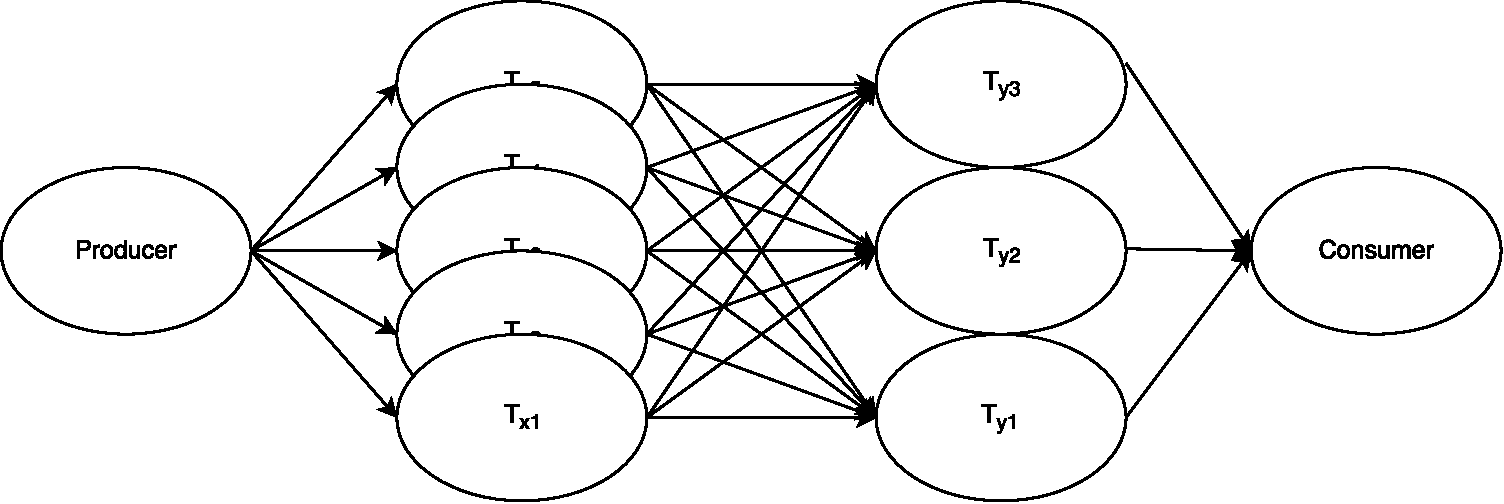
\includegraphics[scale=0.5]{images/extended_app_model_replication.pdf}
\caption[Data flow at replication]{The data flow when two tasks, \emph{T1} and \emph{T2} with different required reliability are replicated.} \label[app]{fig:extended_app_model}
\end{figure}

\begin{figure}[!hbt]
\centering
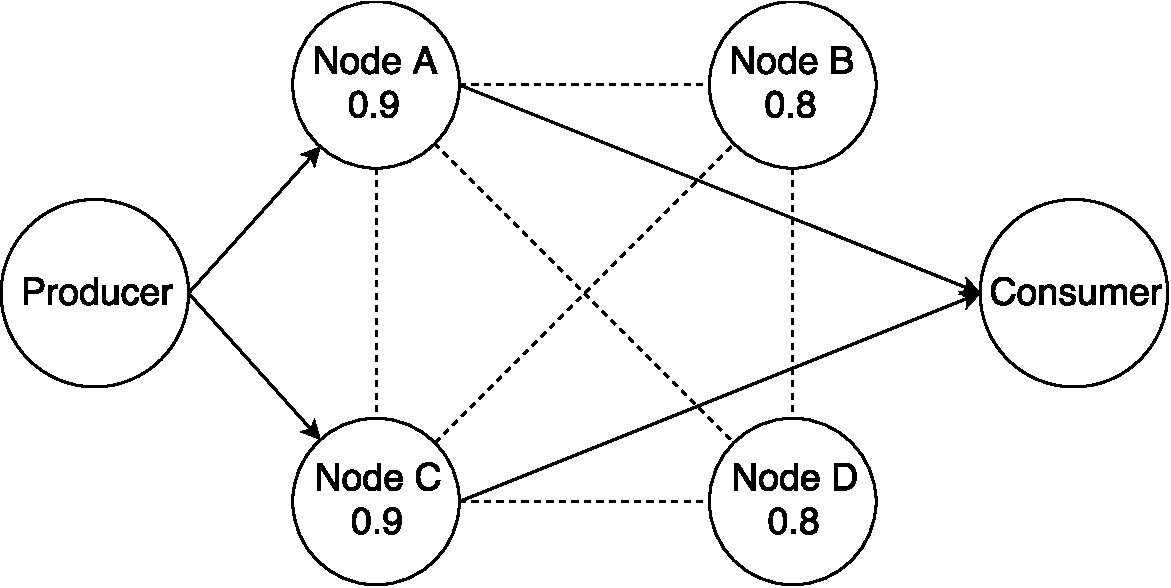
\includegraphics[scale=0.5]{images/before_node_failure.pdf}
\caption[System before a node failure]{Before a node failure. Here two replicas (placed on Node A and C) is required to achieve required reliability.} \label[app]{fig:before_node_failure}
\end{figure}

\begin{figure}[!hbt]
\centering
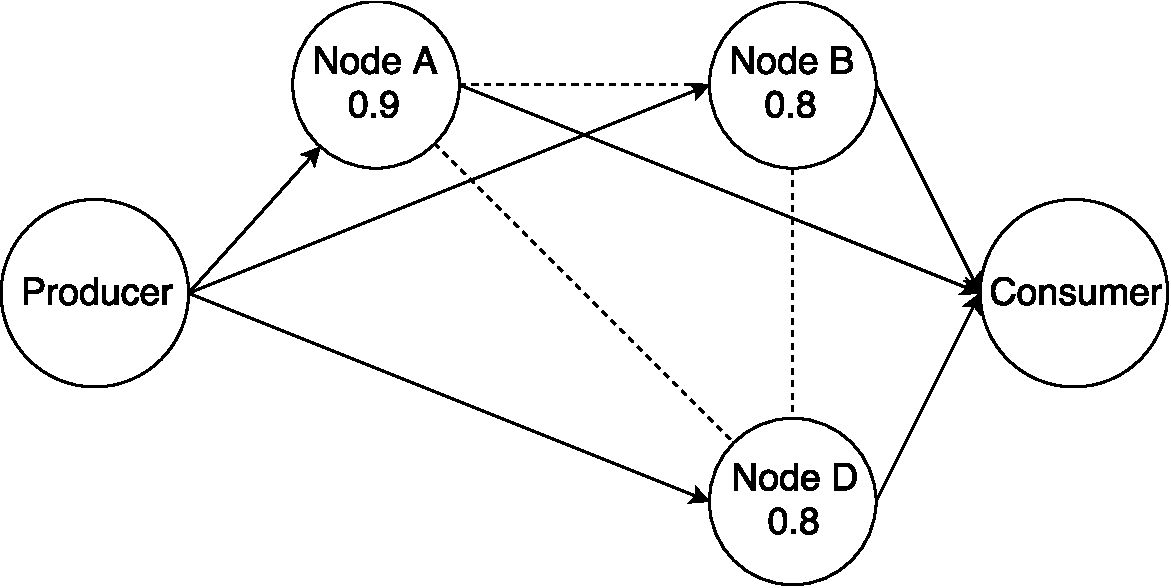
\includegraphics[scale=0.5]{images/after_node_failure.pdf}
\caption[System after a node failure]{After Node C has failed. Now three replicas (placed on Node A, B and D) is required to achieve required reliability.} \label[app]{fig:after_node_failure}
\end{figure}

%TODO change to exclude actors here as well? Or say that this is how it's done in Calvin.
\begin{figure}[!hbt]
\centering
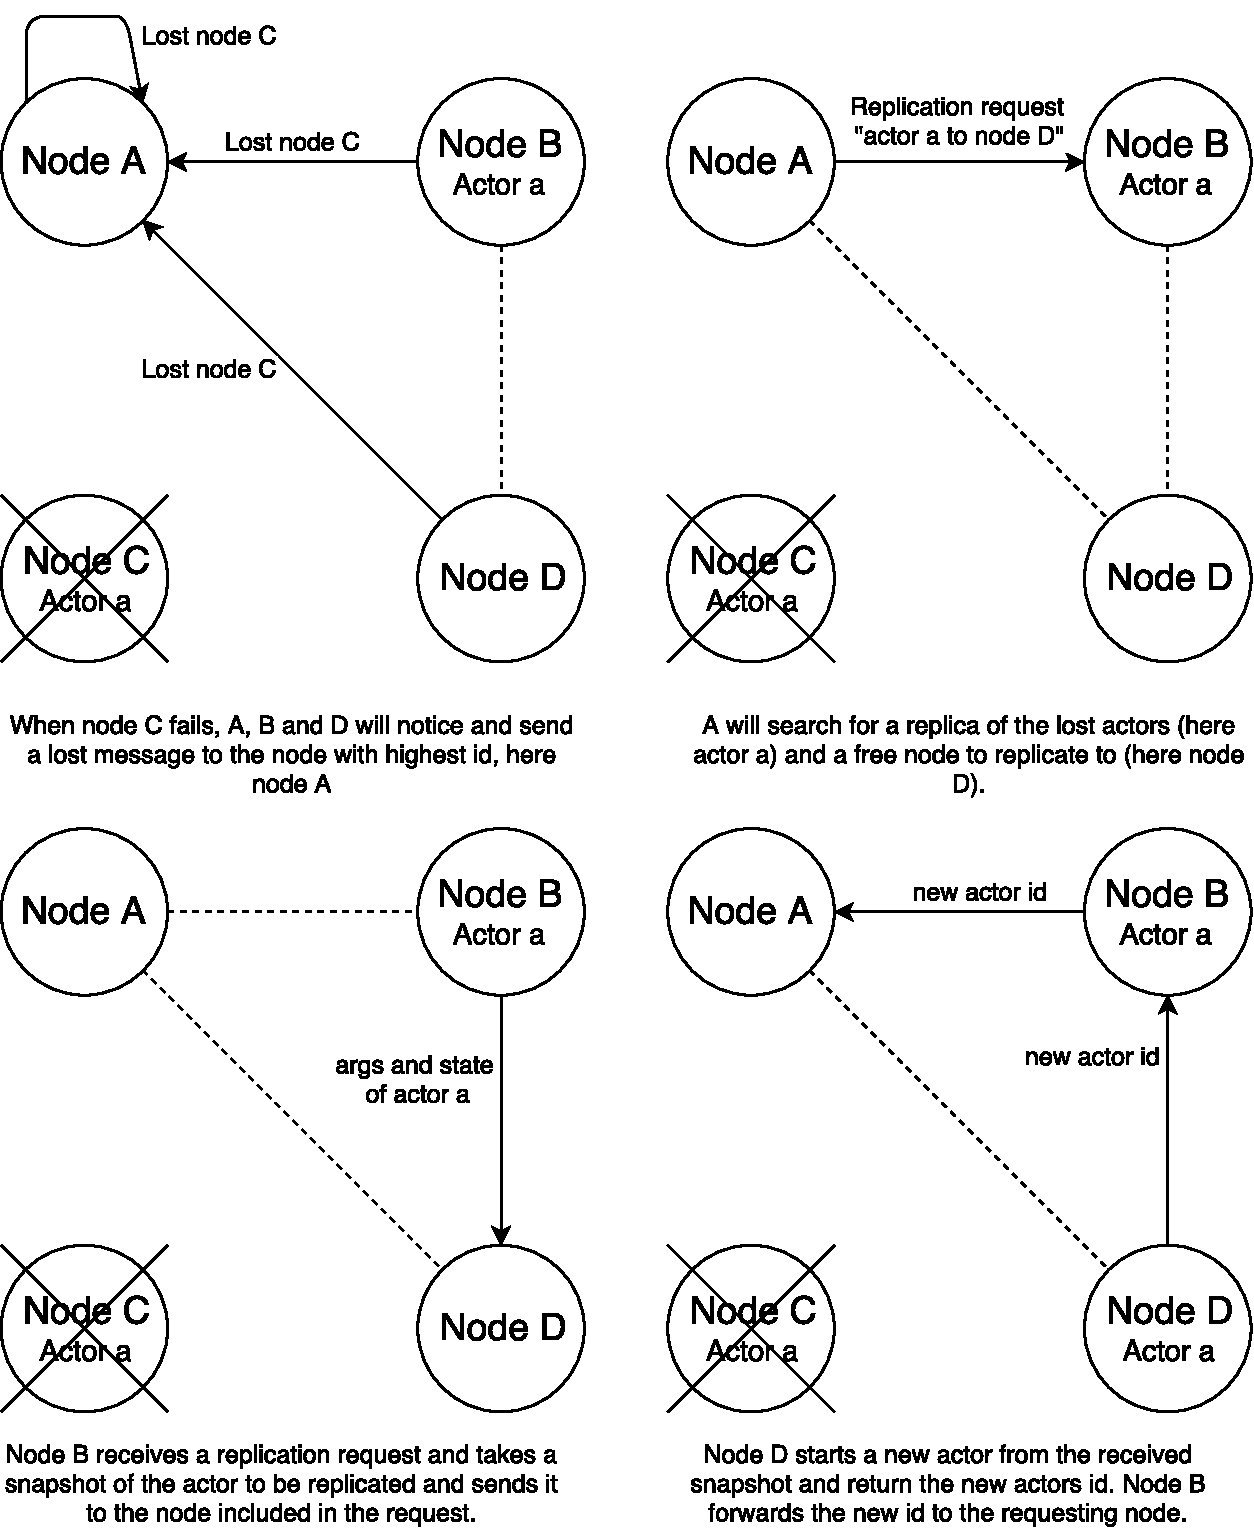
\includegraphics[scale=0.5]{images/replication_flow.pdf}
\caption[Communication after a node failure]{The most important parts of the communication after a node has failed.} \label[app]{fig:replication_flow}
\end{figure}

\begin{figure}[!hbt]
\centering
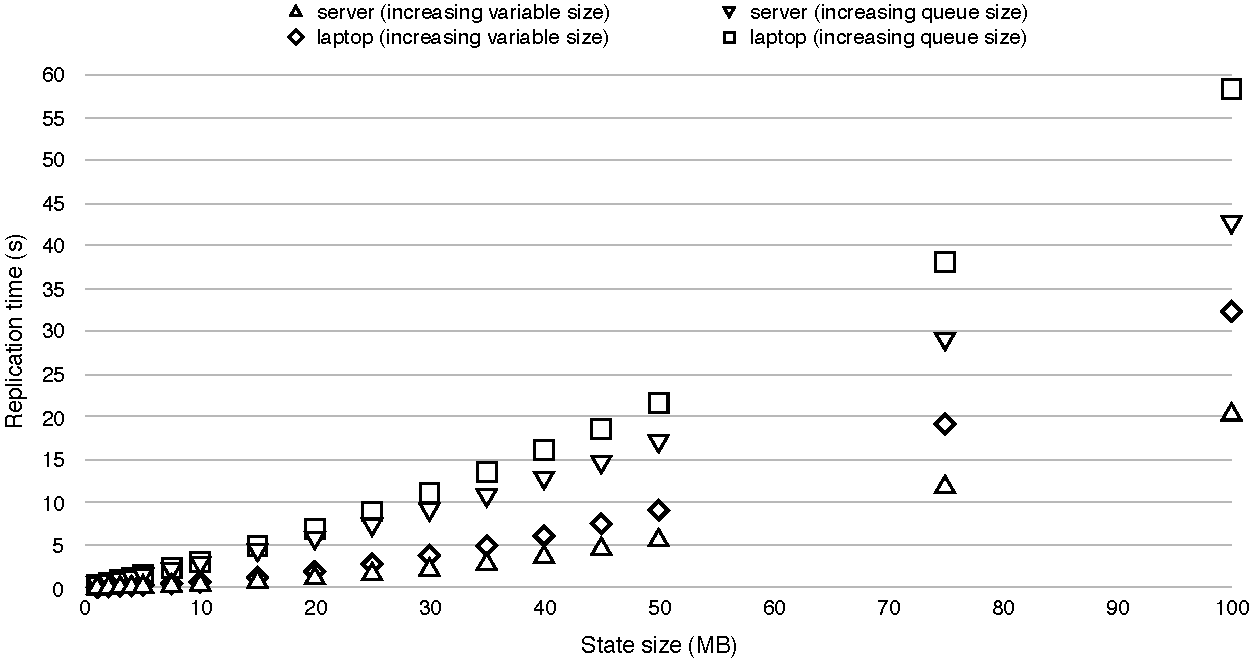
\includegraphics[scale=0.5]{images/results/replication_time/less_than_100.pdf} 
\caption[Average replication time with varying state size]{The average replication time as a function of state size.}\label[app]{fig:replication_time_less_than_100}
\end{figure}

\begin{figure}[!hbt]
\centering
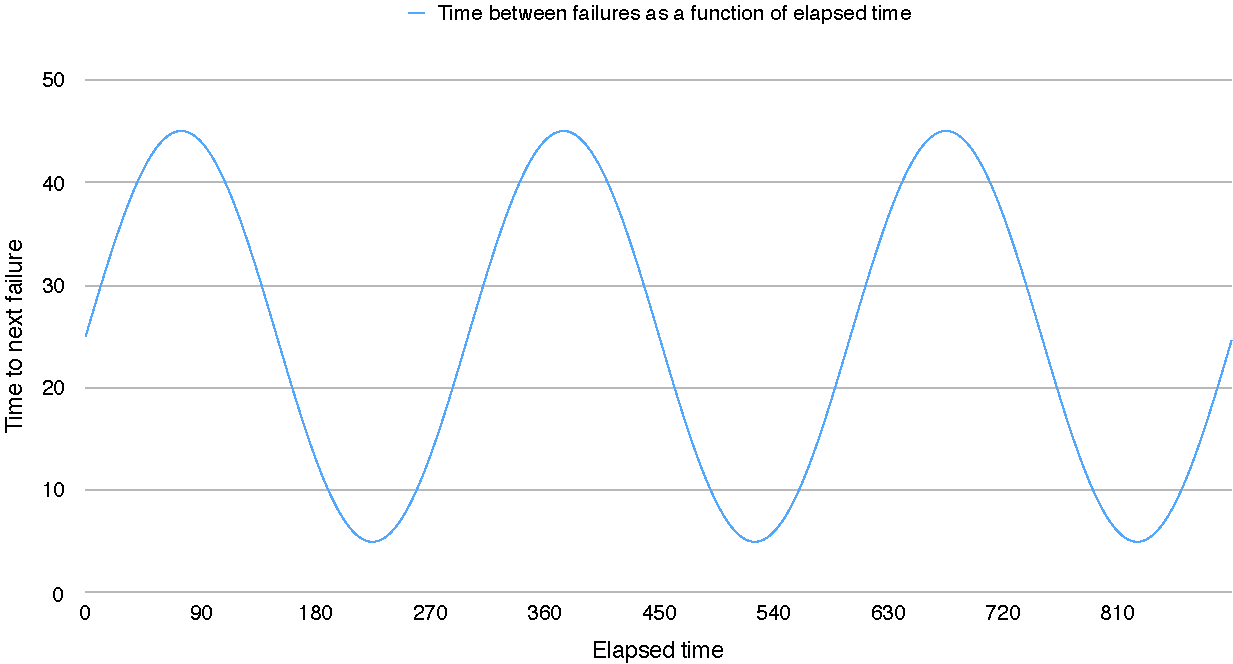
\includegraphics[scale=0.5]{images/sinus_failure_times.pdf}
\caption[Time between failures in~\cref{sec:eval_adaptive_rel_model}]{Time between failures as of~\cref{eq:eval_sleep_time} used in~\cref{sec:eval_adaptive_rel_model}.} \label[app]{fig:eval_sleep_time}
\end{figure}

\begin{figure}[!hbt]
\centering
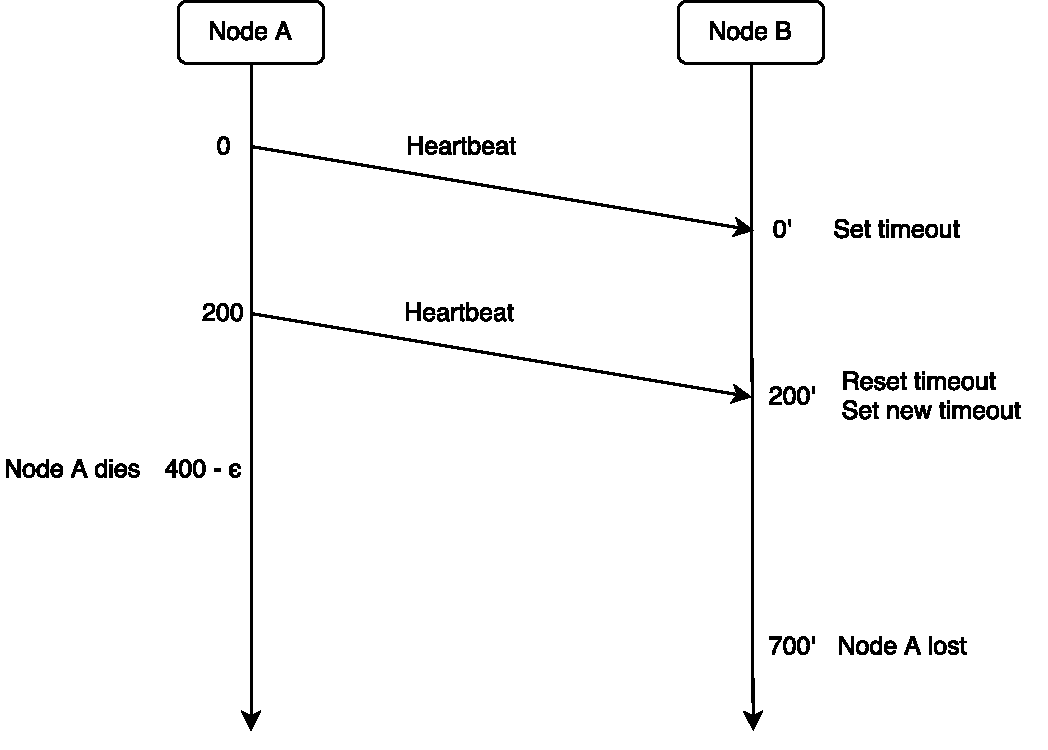
\includegraphics[scale=0.5]{images/heartbeats_best_case.pdf}
\caption[Node failure detecting time, best case]{Best case scenario for detecting a node failure. Node A fails just before sending a heartbeat. The actual detection time, $t_d$ is therefore close to $t_{timeout} - t_h$.} \label[app]{fig:heartbeats_best_case}
\end{figure}

\begin{figure}[!hbt]
\centering
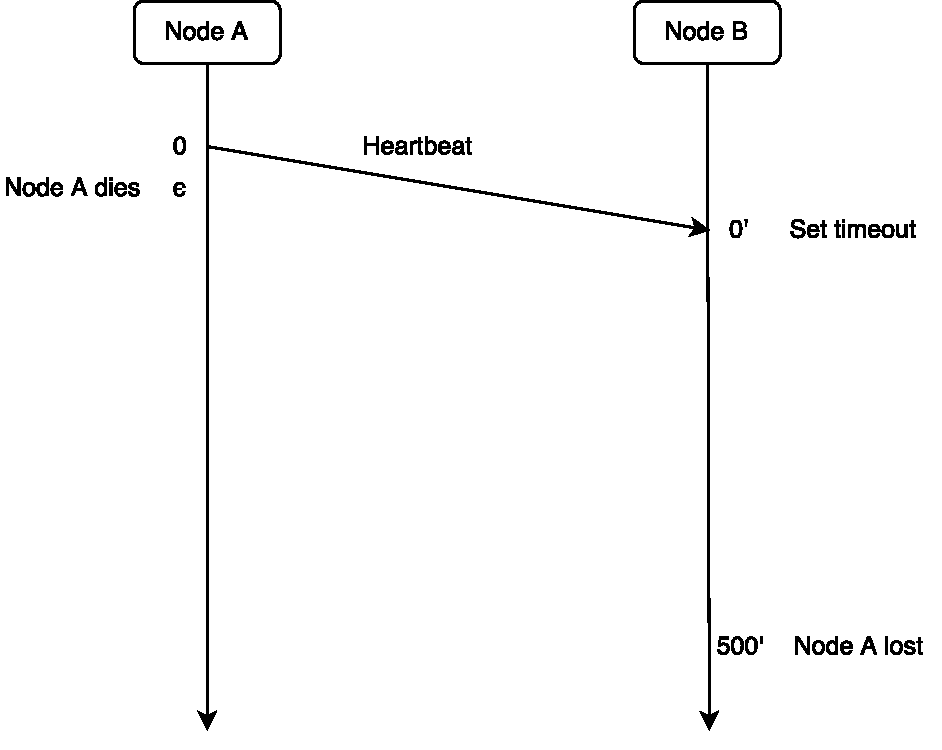
\includegraphics[scale=0.5]{images/heartbeats_worst_case.pdf}
\caption[Node failure detecting time, worst case]{Worst case scenario for detecting a node failure. Node A fails directly after sending a heartbeat. The actual detection time, $t_d$ is therefore close to $t_{timeout}$.} \label[app]{fig:heartbeats_worst_case}
\end{figure}

\iffalse
\chapter{Code} \label{appendix:code}
\fi

\end{appendices}









\iffalse

% Below is the report template found online

\chapter[Short on Formatting]{Formatting}
Avoid empty spaces between \textit{chapter}-\textit{section}, \textit{section}-\textit{sub-section}. For instance, a very brief summary of the chapter would be one way of bridging the chapter heading and the first section of that chapter.
\section{Page Size and Margins}
Use A4 paper, with the text margins given in Table \ref{tab:margins}.
\begin{table}[!hbt]
\centering
\caption{Text margins for A4.}\label{tab:margins}
\begin{tabular}{cc}
\hline
\textbf{margin} & \textbf{space} \\
\hline 
top & 3.0cm\\ 

bottom & 3.0cm \\ 
 
left (inside) & 2.5cm \\ 

right (outside) & 2.5cm \\ 

binding offset & 1.0cm \\ 
\hline 
\end{tabular} 
\end{table}

\section{Typeface and Font Sizes}
The fonts to use for the reports are \textbf{TeX Gyre Termes} (a \textbf{Times New Roman} clone) for serif fonts, \textsf{\textbf{TeX Gyre Heros}} (a \textsf{\textbf{Helvetica}} clone) for sans-serif fonts, and finally \texttt{\textbf{TeX Gyre Cursor}} (a \texttt{\textbf{Courier}} clone) as mono-space font. All these fonts are included with the TeXLive 2013 installation. Table \ref{tab:fonts} lists the most important text elements and the associated fonts.
\begin{table}[!hbt]
\caption{Font types, faces and sizes to be used.}\label{tab:fonts}

 \begin{tabular}{ l c c c}
\hline 
\textbf{Element} & \textbf{Face} & \textbf{Size} & \textbf{\LaTeX size} \\ 
\hline 
{\huge \textbf{Ch. label}} & {\huge \textbf{serif, bold}} & \thefontsize\huge & \verb+\huge+ \\ 
{\Huge \textbf{Chapter}} & {\Huge \textbf{serif, bold}} & \thefontsize\Huge & \verb+\Huge+ \\ 
{\LARGE \textsf{\textbf{Section}}} & {\Large \textsf{\textbf{sans-serif, bold}}} & \thefontsize\LARGE & \verb+\LARGE+ \\ 
{\Large \textsf{\textbf{Subsection}}} & {\Large \textsf{\textbf{sans-serif, bold}}} & \thefontsize\Large & \verb+\Large+ \\ 
{\large \textsf{\textbf{Subsubsection}}} & {\Large \textsf{\textbf{sans-serif, bold}}} & \thefontsize\large & \verb+\large+ \\ 
Body & serif & \thefontsize\normalsize & {\footnotesize \verb+\normalsize+} \\
%{\footnotesize Footnote} & serif & \thefontsize\footnotesize & {\footnotesize \verb+\footnotesize+} \\
{\footnotesize \textsc{Header}} & {\footnotesize \textsc{serif, SmallCaps}} & \thefontsize\footnotesize & \\
Footer (page numbers) & serif, regular & \thefontsize\normalsize & \\
\hline
\textbf{Figure label} & \textbf{serif, bold} & \thefontsize\normalsize & \\
Figure caption & serif, regular & \thefontsize\normalsize & \\
\textsf{In figure} & \textsf{sans-serif} & \textit{any} & \\
\textbf{Table label} & \textbf{serif, bold} & \thefontsize\normalsize & \\
Table caption and text & serif, regular & \thefontsize\normalsize & \\
\texttt{Listings} & \texttt{mono-space} & $\le$ \thefontsize\normalsize & \\
\hline 
\end{tabular} 
\end{table}

\subsection{Headers and Footers}
Note that the page headers are aligned towards the outside of the page (right on the right-hand page, left on the left-hand page) and they contain the section title on the right and the chapter title on the left respectively, in \textsc{SmallCaps}. The footers contain only page numbers on the exterior of the page, aligned right or left depending on the page. The lines used to delimit the headers and footers from the rest of the page are $0.4 pt$ thick, and are as long as the text.

\subsection{Chapters, Sections, Paragraphs}
Chapter, section, subsection, etc. names are all left aligned, and numbered as in this document. 

Chapters always start on the right-hand page, with the label and title separated from the rest of the text by a $0.4 pt$ thick line.

Paragraphs are justified (left and right), using single line spacing. Note that the first paragraph of a chapter, section, etc. is not indented, while the following are indented.

\subsection{Tables}
Table captions should be located above the table, justified, and spaced 2.0cm from left and right (important for very long captions). Tables should be numbered, but the numbering is up to you, and could be, for instance:
\begin{itemize}
\item \textbf{Table X.Y} where X is the chapter number and Y is the table number within that chapter. (This is the default in \LaTeX. More on {\LaTeX} can be found on-line, including whole books, such as \cite{goossens93}.) or
\item \textbf{Table Y} where Y is the table number within the whole report
\end{itemize}
As a recommendation, use regular paragraph text in the tables, bold headings and avoid vertical lines (see Table \ref{tab:fonts}). 

\subsection{Figures}
Figure labels, numbering, and captions should be formed similarly to tables. As a recommendation, use vector graphics in figures (Figure \ref{fig:vectorg}), rather than bitmaps (Figure \ref{fig:rasterg}). Text within figures usually looks better with sans-serif fonts.
\begin{figure}[!hbt]
\centering

\includegraphics[scale=2.5]{images/examplepic1.pdf} 
\caption{A PDF vector graphics figure. Notice the numbering and placement of the caption. The caption text is indented 2.0cm from both left and right text margin.}\label{fig:vectorg}
\end{figure}

\begin{figure}[!hbt]
\centering

\includegraphics[scale=2.5]{images/examplepic3.jpg} 
\caption{A JPEG bitmap figure. Notice the bad quality of such an image when scaling it. Sometimes bitmap images are unavoidable, such as for screen dumps.}\label{fig:rasterg}
\end{figure}
For those interested in delving deeper into the design of graphical information display, please refer to books such as \cite{Tufte:1986, few2012show}.

\section{Mathematical Formulae and Equations}
You are free to use in-text equations and formulae, usually in \textit{italic serif} font. For instance: $S = \sum_i a_i$. We recommend using numbered equations when you do need to refer to the specific equations:
\begin{equation}
E = \int_0^{\delta} P(t) dt \quad \longleftrightarrow \quad E = m c^2
\end{equation}
The numbering system for equations should be similar to that used for tables and figures.

\section{References}
Your references should be gathered in a \textbf{References} section, located at the end of the document (before \textbf{Appendices}). We recommend using number style references, ordered as appearing in the document or alphabetically. Have a look at the references in this template in order to figure out the style, fonts and fields. Web references are acceptable (with restraint) as long as you specify the date you accessed the given link \cite{fontspec, CTAN}. You may of course use URLs directly in the document, using mono-space font, i.e. \url{http://cs.lth.se/}.

\section{Colours}
As a general rule, all theses are printed in black-and-white, with the exception of selected parts in selected theses that need to display colour images essential to describing the thesis outcome (\textit{computer graphics}, for instance).

A strong requirement is for using \textbf{black text on white background} in your document's main text. Otherwise we do encourage using colours in your figures, or other elements (i.e. the colour marking internal and external references) that would make the document more readable on screen. You may also emphasize table rows, columns, cells, or headers using white text on black background, or black text on light grey background.

Finally, note that the document should look good in black-and-white print. Colours are often rendered using monochrome textures in print, which makes them look different from on screen versions. This means that you should choose your colours wisely, and even opt for black-and-white textures when the distinction between colours is hard to make in print. The best way to check how your document looks, is to print out a copy yourself.

\chapter{Language}

You are strongly encouraged to write your report in English, for two reasons. First, it will improve your use of English language. Second, it will increase visibility for you, the author, as well as for the Department of Computer Science, and for your host company (if any).

However, note that your examiner (and supervisors) are not there to provide you with extensive language feedback. We recommend that you check the language used in your report in several ways:
\begin{description}
\item[Reference books] dedicated to language issues can be very useful. \cite{heffernan2000writing} 
\item[Spelling and grammar checkers] which are usually available in the commonly used text editing environments.
\item[Colleagues and friends] willing to provide feedback your writing.
\item[Studieverkstaden] is a university level workshop, that can help you with language related problems (see \href{http://www.lu.se/studera/livet-som-student/service-och-stod/studieverkstaden}{Studieverkstaden}'s web page).
\item[Websites] useful for detecting language errors or strange expressions, such as
\begin{itemize}
\item \url{http://translate.google.com}
\item \url{http://www.gingersoftware.com/grammarcheck/}
\end{itemize}
\end{description}

\section{Style Elements}
Next, we will just give some rough guidelines for good style in a report written in English. Your supervisor and examiner as well as the aforementioned \textbf{Studieverkstad} might have a different take on these, so we recommend you follow their advice whenever in doubt. If you want a reference to a short style guide, have a look at \cite{shortstyleguide}.

\subsubsection{Widows and Orphans}

Avoid \textit{widows} and \textit{orphans}, namely words or short lines at the beginning or end of a paragraph, which are left dangling at the top or bottom of a column, separated from the rest of the paragraph.

\subsubsection{Footnotes}

We strongly recommend you avoid footnotes. To quote from \cite{OGSW}, \textit{Footnotes are frequently misused by containing information which should either be placed in the text or excluded altogether. They should be avoided as a general rule and are acceptable only in exceptional cases when incorporation of their content in the text [is] not possible.} 

\subsubsection{Active vs. Passive Voice}

Generally active voice (\textit{I ate this apple.}) is easier to understand than passive voice (\textit{This apple has been eaten (by me).}) In passive voice sentences the actor carrying out the action is often forgotten, which makes the reader wonder who actually performed the action. In a report is important to be clear about who carried out the work. Therefore we recommend to use active voice, and preferably the plural form \textit{we} instead of \textit{I} (even in single author reports).

\subsubsection{Long and Short Sentences}
A nice brief list of sentence problems and solutions is given in \cite{yalesentences}. Using choppy sentences (too short) is a common problem of many students. The opposite, using too long sentences, occurs less often, in our experience.

\subsubsection{Subject-Predicate Agreement}
A common problem of native Swedish speakers is getting the subject-predicate (verb) agreement right in sentences. Note that a verb must agree in person and number with its subject. As a rough tip, if you have subject ending in \textit{s} (plural), the predicate should not, and the other way around. Hence, \textit{only one s}. Examples follow:
\begin{description}
\item[incorrect] He have to take this road.
\item[correct] He has to take this road.
\end{description}
\begin{description}
\item[incorrect] These words forms a sentence.
\item[correct] These words form a sentence.
\end{description}
\noindent In more complex sentences, getting the agreement right is trickier. A brief guide is given in the \textit{20 Rules of Subject Verb Agreement} \cite{subjectverb}.

\chapter{Structure}
It is a good idea to discuss the structure of the report with your supervisor rather early in your writing. Given next is a generic structure that is a starting point, but by no means the absolute standard. Your supervisor should provide a better structure for the specific field you are writing your thesis in. Note also that the naming of the chapters is not compulsory, but may be a helpful guideline.
\begin{description}
\item[Introduction] should give the background of your work. Important parts to cover:
\begin{itemize}
\item Give the context of your work, have a short introduction to the area.
\item Define the problem you are solving (or trying to solve).
\item Specify your contributions. What does this particular work/report bring to the research are or to the body of knowledge? How is the work divided between the co-authors? (This part is essential to pinpoint individual work. For theses with two authors, it is compulsory to identify which author has contributed with which part, both with respect to the work and the report.)
\item Describe related work (literature study). Besides listing other work in the area, mention how is it related or relevant to your work. The tradition in some research area is to place this part at the end of the report (check with your supervisor).
\end{itemize}
\item[Approach] should contain a description of your solution(s), with all the theoretical background needed. On occasion this is replaced by a subset or all of the following:
\begin{itemize}
\item \textbf{Method}: describe how you go about solving the problem you defined. Also how do you show/prove that your solution actually works, and how well does it work.
\item \textbf{Theory}: should contain the theoretical background needed to understand your work, if necessary.
\item \textbf{Implementation}: if your work involved building an artefact/implementation, give the details here. Note, that this should not, as a rule, be a chronological description of your efforts, but a view of the result. There is a place for insights and lamentation later on in the report, in the Discussion section.
\end{itemize}
\item[Evaluation] is the part where you present the finds. Depending on the area this part contains a subset or all of the following: 
\begin{itemize}
\item \textbf{Experimental Setup} should describe the details of the method used to evaluate your solution(s)/approach. Sometimes this is already addressed in the \textbf{Method}, sometimes this part replaces \textbf{Method}.
\item \textbf{Results} contains the data (as tables, graphs) obtained via experiments (benchmarking, polls, interviews).
\item \textbf{Discussion} allows for a longer discussion and interpretation of the results from the evaluation, including extrapolations and/or expected impact. This might also be a good place to describe your positive and negative experiences related to the work you carried out.
\end{itemize} 
Occasionally these sections are intermingled, if this allows for a better presentation of your work. However, try to distinguish between measurements or hard data (results) and extrapolations, interpretations, or speculations (discussion).
\item[Conclusions] should summarize your findings and possible improvements or recommendations.
\item[Bibliography] is a must in a scientific report. {\LaTeX} and \texttt{bibtex} offer great support for handling references and automatically generating bibliographies.
\item[Appendices] should contain lengthy details of the experimental setup, mathematical proofs, code download information, and shorter code snippets. Avoid longer code listings. Source code should rather be made available for download on a website or on-line repository of your choosing.

\end{description}
\makebibliography{MyMSc}

\begin{appendices}
\chapter{About This Document}
The following environments and tools were used to create this document:
\begin{itemize}
\item operating system: Mac OS X 10.10.1
\item tex distribution: MacTeX-2014, \url{http://www.tug.org/mactex/}
\item tex editor: Texmaker 4.4.1 for Mac, \url{http://www.xm1math.net/texmaker/} for its XeLaTeX flow (recommended) or pdfLaTeX flow
\item bibtex editor: BibDesk 1.6.3 for Mac, \url{http://bibdesk.sourceforge.net/}
\item fonts \texttt{cslthse-msc.cls} document class): 
\begin{description}
\item{for XeLaTeX}: TeX Gyre Termes, \textsf{TeX Gyre Heros}, \texttt{TeX Gyre Cursor} (installed from the TeXLive 2013)
\item{for pdfLaTeX}: TeX Gyre font packages: tgtermes.sty, tgheros.sty, tgcursor.sty, gtxmath.sty (available through TeXLive 2013) 
\end{description} 
\item picture editor: OmniGraffle Professional 5.4.2
\end{itemize}

\noindent A list of the essential \LaTeX packages needed to compile this document follows (all except \texttt{hyperref} are included in the document class):
\begin{itemize}
\item \texttt{fontspec}, to access local fonts, needs the XeLaTeX flow
\item \texttt{geometry}, for page layout
\item \texttt{titling}, for formatting the title page
\item \texttt{fancyhdr}, for custom headers and footers
\item \texttt{abstract}, for customizing the abstract
\item \texttt{titlesec}, for custom chapters, sections, etc.
\item \texttt{caption}, for custom tables and figure captions
\item \texttt{hyperref}, for producing PDF with hyperlinks
\item \texttt{appendix}, for appendices
\item \texttt{printlen}, for printing text sizes
\item \texttt{textcomp}, for text companion fonts (e.g. bullet)
\end{itemize}

\noindent Other useful packages:
\begin{itemize}
\item \texttt{listings}, for producing code listings with syntax colouring and line numbers
\end{itemize}

\chapter{List of Changes}
\subsubsection{Since 2015/04/27}
\begin{itemize}
\item Improved the \textbf{Structure} chapter and added more detailed comments for each part.
\end{itemize}

\subsubsection{Since 2014/02/18}
\begin{itemize}
\item Added the possibility to specify two supervisors. Use either of the \verb+\supervisor{}+ or \verb+\supervisors{}{}+ commands to set the names and contacts on the first page.
\end{itemize}

\subsubsection{Since 2013/09/23}
\begin{itemize}
\item Added missing colon ":" after \textit{Examiner} on the front page. 
\end{itemize}

\subsubsection{Since 2013/08/30}
\begin{itemize}
\item Changed fonts from Garamond (Times New Roman), Helvetica (Arial), Courier (Source Code Pro) to Tex Gyre fonts, namely Termes, Heros, Cursor, which are freely available with TexLive 2013 installation. These are all clones of Times New Roman, Helvetica and Courier, respectively. Garamond is problematic on some systems, being a non-freely available font.
\item Corrected the \textit{Face} column in Table \ref{tab:fonts} to correctly depict the font face.
\end{itemize}

\subsubsection{Since 2013/02/22}
\begin{itemize}
\item Number of words required in the abstract changed to 150 (from 300).
\end{itemize}

\subsubsection{Since 2013/02/15}
\begin{itemize}
\item Made a separate document class, for clarity.
\item made it work with pdfLaTeX and garamond.sty, in addition to XeLaTeX and true type fonts. It is up to the user to get the hold of the garamond.zip from \url{http://gael-varoquaux.info/computers/garamond/index.html}.
\end{itemize}
\end{appendices}

\fi

\end{document}
